\documentclass[
	12pt,
	openright,
	twoside,
	a4paper,
	english,
	brazil
	]{abntex2}

\usepackage{lmodern}
\usepackage[T1]{fontenc}
\usepackage[utf8]{inputenc}
\usepackage{indentfirst}
\usepackage{color}
\usepackage{float}
\usepackage{graphicx}
\usepackage{microtype}
\usepackage[brazilian,hyperpageref]{backref}
\usepackage[alf]{abntex2cite}
\usepackage{amsmath}
\usepackage{ufsc}
\usepackage{listings}
\usepackage{cleveref}
\usepackage{multirow}
\usepackage{longtable}
\usepackage{pdfpages}

\renewcommand{\backrefpagesname}{Citado na(s) página(s):~}
\renewcommand{\backref}{}
\renewcommand*{\backrefalt}[4]{
	\ifcase #1
		Nenhuma citação no texto.
	\or
		Citado na página #2.
	\else
		Citado #1 vezes nas páginas #2.
	\fi}

%------------------------------------------------------------------------------%

\titulo{Dinâmica para identificação e análise de riscos em equipes ágeis}
\autor{Amanda Martins Oliveira}
\local{Florianópolis, Brasil}
\data{2025}
\orientador{Jean Carlo Rossa Hauck}
\instituicao{
  Universidade de Santa Catarina -- UFSC
  \par
  Ciências da Computação
  \par
  Programa de Graduação}
\tipotrabalho{Tese (Bacharel)}
\preambulo{Trabalho de Conclusão de Curso submetido ao curso de Ciências da Computação como requisito para a obtenção do Grau de Bacharel em Ciências da Computação.}

% ABNT ------------------------------------------------------------------------%

\graphicspath{ {./images/} }
\definecolor{blue}{RGB}{41,5,195}

\makeatletter
  \hypersetup{
    pdftitle={\@title},
    pdfauthor={\@author},
    pdfsubject={\imprimirpreambulo},
    pdfcreator={LaTeX with abnTeX2},
    pdfkeywords={abnt}{latex}{abntex}{abntex2}{trabalho acadêmico},
    colorlinks=true,
    linkcolor=blue,
    citecolor=blue,
    filecolor=magenta,
    urlcolor=blue,
    bookmarksdepth=4
  }
\makeatother

\makeatletter
  \setlength{\@fptop}{5pt}
\makeatother

\setlength{\parindent}{1.3cm}
\setlength{\parskip}{0.2cm}

% Other settings --------------------------------------------------------------%

\crefformat{footnote}{#2\footnotemark[#1]#3}
\lstset{
  basicstyle=\small\ttfamily,
  columns=flexible,
  breaklines=true,
  literate=
    {á}{{\'a}}1
    {à}{{\`a}}1
    {ã}{{\~a}}1
    {é}{{\'e}}1
    {ê}{{\^e}}1
    {í}{{\'i}}1
    {ó}{{\'o}}1
    {õ}{{\~o}}1
    {ú}{{\'u}}1
    {ü}{{\"u}}1
    {ç}{{\c{c}}}1
}

%------------------------------------------------------------------------------%

\makeindex

%------------------------------------------------------------------------------%

\begin{document}
\selectlanguage{brazil}
\frenchspacing

%------------------------------------------------------------------------------%

\imprimircapa

%------------------------------------------------------------------------------%

\imprimirfolhaderosto*

%------------------------------------------------------------------------------%

\setlength{\absparsep}{18pt}
\begin{resumo}
  Com a popularização dos métodos ágeis cada vez mais organizações adotam este abordagem pela flexibilidade  e adaptabilidade proposta pelo modelo. Entretanto, apesar destas vantagens o uso destes métodos traz consigo desafios relacionados à gestão de riscos nos projetos, já que frequentemente não possuem um processo explícito para tal gerenciamento.
  O objetivo deste trabalho é analisar, desenvolver, aplicar e avaliar uma dinâmica que auxilie no processo de gestão de riscos, por meio de um estudo de caso aplicado em equipes ágeis e em sala de aula. A proposta é criar uma maneira lúdica e facilitada de gerenciamento de riscos, adaptada para ambientes ágeis.
  Para isto o trabalho será baseado em uma estrutura que inicia com uma fundamentação teórica e a análise do estado da arte sobre a gestão de riscos em metodologias ágeis. Com base nessa análise, será desenvolvida uma dinâmica para gestão de riscos no contexto ágil. Em seguida, a eficácia dessa dinâmica será avaliada por meio da aplicação em estudos de caso com equipes de desenvolvimento de \textit{software} e em cenários educacionais, como salas de aula.
  Espera-se com isso o desenvolvimento e a validação de uma dinâmica lúdica que auxilie os profissionais que utilizam metodologias ágeis na análise e identificação de riscos. Acredita-se que, com essa abordagem, será possível mitigar impactos negativos potenciais nos projetos, promovendo uma entrega de valor contínua e eficiente pelas equipes que integrarem a ferramenta ao seu processo. 
  \vspace{\onelineskip}

  \noindent\textbf{Palavras-chave}: Gestão de Riscos, Gestão de Projetos, Métodos Ágeis.

\end{resumo}

%------------------------------------------------------------------------------%

\begin{resumo}[Abstract]
  \begin{otherlanguage*}{english}
    With the popularization of agile methods, an increasing number of organizations are adopting this approach due to the flexibility and adaptability proposed by the model. However, despite these advantages, the use of these methods brings challenges related to risk management in projects, as they often lack an explicit process for such management.
    The objective of this study is to analyze, develop, apply, and evaluate a framework that aids the risk management process through a case study applied to agile teams and in classroom settings. The proposal is to create a playful and simplified way of managing risks, adapted for agile environments.
    To achieve this, the work will be based on a structure that begins with a theoretical foundation and an analysis of the state of the art regarding risk management in agile methodologies. Based on this analysis, a risk management framework will be developed for the agile context. Subsequently, the effectiveness of this framework will be evaluated through application in case studies with software development teams and in educational scenarios, such as classrooms.
    The aim is to develop and validate a playful framework that assists professionals using agile methodologies in the analysis and identification of risks. It is believed that this approach will help mitigate potential negative impacts on projects, promoting continuous and efficient value delivery by teams that integrate the tool into their processes.
    \vspace{\onelineskip}

    \noindent\textbf{Keywords}: Risk management, Project Management, Agile Methods.
  \end{otherlanguage*}
\end{resumo}

% Figuras ---------------------------------------------------------------------%

\pdfbookmark[0]{\listfigurename}{lof}
\listoffigures*
\cleardoublepage

% Quadros ---------------------------------------------------------------------%

% \pdfbookmark[0]{\listofquadrosname}{loq}
% \listofquadros*
% \cleardoublepage

% Tabelas ---------------------------------------------------------------------%

\pdfbookmark[0]{\listtablename}{lot}
\listoftables*
\cleardoublepage

% Siglas ----------------------------------------------------------------------%

\begin{siglas}
  \item[MSL] Mapeamento Sistemático de Literatura
  \item[XP] eXtreme Programming
  \item[DAD] Disciplined Agile Delivery 
  \item[SAFe] Scaled Agile Framework
  \item[PMBOK] Project Management Body of Knowledge
  \item[CMMI] Capability Maturity Model Integration
  \item[ISO] International Organization for Standardization
  \item[IEC] International Electrotechnical Commission
  \item[IEEE] Institute of Electrical and Electronics Engineers
  \item[SEI] Software Engineering Institute
  \item[EAP] Estrutura Analítica do Projeto
\end{siglas}

% Sumário ---------------------------------------------------------------------%

\pdfbookmark[0]{\contentsname}{toc}
\tableofcontents*
\cleardoublepage
\textual

%------------------------------------------------------------------------------%

\chapter{Introdução e objetivos} % Ideias gerais e por quê fazer?

\section{Introdução}

As metodologias ágeis têm se consolidado como uma das abordagens mais eficazes e flexíveis para o desenvolvimento de \textit{software} e a gestão de projetos na área de tecnologia \cite{AgileManifest, AgileGuide}. Frameworks como \textit{Scrum}, \textit{Kanban} e \textit{XP} são amplamente adotados por promoverem adaptação rápida a mudanças, comunicação contínua com o cliente e entrega incremental de valor \cite{Poppendieck_Poppendieck_2003, Pressman_2014}.

Entretanto, um dos desafios associados a essas práticas é a gestão de riscos, que, embora reconhecida como essencial para o sucesso de projetos de software \cite{PMBOK, iso16085}, muitas vezes não é realizada de maneira estruturada ou explícita em contextos ágeis. Essa ausência pode deixar equipes vulneráveis a imprevistos que impactam negativamente prazos, custos e qualidade do produto \cite{Afshari, Zahedi}.

O problema identificado neste trabalho é que muitas equipes ágeis não adotam processos sistemáticos de gerenciamento de riscos, o que contribui para a repetição de falhas que poderiam ser mitigadas ou evitadas. Considerando esse cenário, a hipótese central é que a criação e implementação de uma dinâmica lúdica, acessível e facilitada para a gestão de riscos pode apoiar as equipes ágeis na identificação e análise de riscos, resultando em entregas mais consistentes e resilientes.

Esta pesquisa se justifica pela lacuna existente na integração de práticas explícitas de gestão de riscos ao contexto das metodologias ágeis \cite{LopesSamueldeSouza2022ARMF}. Embora existam modelos tradicionais e frameworks propostos na literatura, muitas dessas abordagens não se adaptam à cultura ágil por exigirem documentação extensa ou processos pesados \cite{Gold}. A proposta de uma dinâmica lúdica se alinha com iniciativas recentes que utilizam jogos sérios para promover engajamento e aprendizado em gestão de projetos de software \cite{SERGE, Caponetto, Alomari}, tornando o processo de identificação de riscos mais colaborativo e intuitivo.

Ao desenvolver e validar uma dinâmica gamificada voltada para esse fim, este trabalho busca contribuir com uma ferramenta prática, replicável e de baixo custo que pode ser adotada por diferentes equipes e organizações. Espera-se que os resultados obtidos incentivem a adoção de práticas mais sistemáticas e acessíveis de gestão de riscos no desenvolvimento ágil de \textit{software}.

\section{Objetivos gerais}

Este trabalho tem o objetivo de analisar, desenvolver, aplicar e avaliar uma dinâmica que auxilie no processo de gestão de riscos por meio de um estudo de caso aplicado em equipes ágeis e em sala de aula.

\section{Objetivos específicos}

\begin{enumerate}
  \item Realizar uma análise da literatura quanto ao estado da arte da gestão de riscos em métodos ágeis, bem como de possíveis dinâmicas criadas para auxiliar nessa gestão.
  \item Desenvolver uma dinâmica que auxilie na identificação e análise de riscos em projetos com equipes ágeis.
  \item Aplicar a dinâmica e avaliar os impactos nas equipes por meio de um estudo de caso.
\end{enumerate}

\section{Método de pesquisa}

\textbf{Etapa 1 -- Fundamentação Teórica}: Nesta etapa serão revisados conceitos fundamentais da literatura relacionados a gerência de projetos, métodos ágeis e gestão de riscos. Esta etapa é composta pelas seguintes atividades:

\begin{itemize}
  \item[] Atividade 1.1: Fundamentar principais conceitos sobre gerência de projeto.
  \item[] Atividade 1.2: Fundamentar principais conceitos sobre métodos ágeis.
  \item[] Atividade 1.3: Fundamentar principais conceitos sobre gestão de riscos.
\end{itemize}


\textbf{Etapa 2 -- Análise do estado da arte}: Nesta etapa será realizada uma revisão sistemática da literatura para o levantamento de estudos correlacionados com o tema deste trabalho. Esta etapa é composta pelas seguintes atividades:

\begin{itemize}
  \item[] Atividade 2.1: Definição do protocolo de pesquisa.
  \item[] Atividade 2.2: Seleção dos estudos.
  \item[] Atividade 2.3: Análise dos resultados.
\end{itemize}

\textbf{Etapa 3 -- Desenvolvimento da dinâmica}: A partir das etapas anteriores, será criada a dinâmica para identificação de análise de riscos em equipe ágeis. Esta etapa é composta pelas seguintes atividades:

\begin{itemize}

  \item[] Atividade 3.1: Identificação de objetivos de negócios.
  \item[] Atividade 3.2: Desenvolver a proposta de solução.
  \item[] Atividade 3.3: Definição do escopo da gamificação e estudo de viabilidade.
  \item[] Atividade 3.4: Análise e design.
  \item[] Atividade 3.5: Desenvolvimento da plataforma gamificada.

\end{itemize}

\textbf{Etapa 4 -- Avaliação da dinâmica e aplicação do estudo de caso}: Nesta etapa final será aplicada a dinâmica desenvolvida na etapa anterior, executando um estudo de caso e realizando a avaliação e validação da mesma. Esta etapa é composta pelas seguintes atividades:


\begin{itemize}
  \item[] Atividade 4.1: Planejamento do estudo de caso.
  \item[] Atividade 4.2: Realização do estudo de caso.
  \item[] Atividade 4.3: Análise dos resultados do estudo de caso.
\end{itemize}

%------------------------------------------------------------------------------%

\chapter{Fundamentação Teórica}
\label{cap:fundamentacao-teorica}


Neste capítulo, serão apresentados conceitos relevantes relacionados à gerência de projetos, gerenciamento de riscos, métodos ágeis e gamificação, que serão abordados ao longo deste trabalho, visando proporcionar uma base sólida para o desenvolvimento e análise do tema.

\section{Gerência de projetos}

O PMBOK \cite{PMBOK} define que o gerenciamento de projetos é a aplicação de conhecimentos, habilidades, ferramentas e técnicas às atividades do projeto a fim de cumprir os seus requisitos. Diversas atividades podem estar envolvidas para alcançar este objetivo, mas para \citeonline{Pressman_2014} todas envolvem planejamento, monitoração e controle de pessoas, processos e eventos que ocorrem à medida que o \textit{software} evolui desde os conceitos preliminares até sua disponibilização operacional e completa.

Por envolver tantas etapas e atividades do projeto, todos os membros possuem algum papel na atividade de gerenciamento, cada um no escopo de suas atividades \cite{Pressman_2014}. Um engenheiro de \textit{software} gerenciará suas atividades diárias, planejando, monitorando e controlando as tarefas técnicas, enquanto o gerente do projeto planeja, monitora e controla o trabalho de uma equipe de engenheiros de \textit{software}.

Como abordado por \citeonline{Sommerville_2007} os projetos precisam ser gerenciados, pois a engenharia de \textit{software} profissional está sempre sujeita a restrições, e esta gestão garante que o projeto de \textit{software} atenda e supere essas restrições, enquanto oferece \textit{software} de qualidade. Além disso, quando aplicados e integrados os processos de gerenciamento apropriados, estas ações permitem que as organizações executem projetos de forma mais eficaz e eficiente \cite{PMBOK}, diminuindo custos e retrabalhos. O alcance desta eficiência permite que as organizações \cite{PMBOK}:

\begin{itemize}
  \item Vinculem os resultados do projeto com os objetivos do negócio;
  \item Concorram com mais eficácia nos seus mercados;
  \item Sustentem a organização;
  \item Respondam ao impacto das mudanças de ambiente de negócios nos projetos, ajustando adequadamente os planos de gerenciamento de projetos.
\end{itemize}
Quando realizada esta gestão eficaz, ela ajuda indivíduos, grupos e organizações públicas e privadas a:

\begin{itemize}
  \item Cumprirem os objetivos do negócio;
  \item Satisfazerem as expectativas das partes interessadas;
  \item Serem mais previsíveis;
  \item Entregarem os produtos certos no momento certo;
  \item Resolverem problemas e questões;
  \item Responderem a riscos em tempo hábil;
  \item Otimizarem o uso dos recursos organizacionais;
  \item Identificarem, recuperarem ou eliminarem projetos com problemas;
  \item Gerenciarem restrições (escopo, qualidade, cronograma, custos, recursos);
  \item Equilibrarem a influência de restrições do projeto (o aumento de escopo pode aumentar custos ou o prazo);
  \item Gerenciarem melhor as mudanças;
  \item Aumentarem suas chances de sucesso.
\end{itemize}

Para \citeonline{Sommerville_2007}, o sucesso do projeto não é garantido por um bom gerenciamento. No entanto, o mau gerenciamento geralmente resulta em falha do projeto. Os critérios de sucesso para o gerenciamento de projetos variam de um projeto para outro \cite{Pressman_2014}, mas, para a maioria dos projetos, estas são as metas mais importantes:

\begin{enumerate}
  \item Fornecer o \textit{software} ao cliente no prazo estabelecido.
  \item Manter os custos gerais dentro do orçamento.
  \item Entregar \textit{software} que atenda às expectativas do cliente.
  \item Manter uma equipe de desenvolvimento que trabalhe bem e feliz.
\end{enumerate}

Para realizar este processo de gerenciamento o PMBOK \cite{PMBOK} categoriza o processo em cinco grupos, que são organizados da seguinte maneira:

\begin{itemize}
  \item \textbf{Iniciação}: contém os processos realizados para definir um novo projeto ou uma nova fase de um projeto obtendo autorização para iniciar o projeto ou a fase. O objetivo principal é alinhar as expectativas das partes interessadas com o objetivo do projeto, informar as partes interessadas sobre o escopo e os objetivos, e discutir como sua participação no projeto e nas fases associadas pode ajudar a garantir que suas expectativas sejam realizadas. Nos processos de iniciação, o escopo inicial é definido e os recursos financeiros iniciais são comprometidos. As partes interessadas que vão interagir e influenciar o resultado geral do projeto são identificadas. Os principais benefícios deste grupo de processos é que somente projetos que estão alinhados com os objetivos estratégicos da organização são autorizados, e que o \textit{business case}, os benefícios e as partes interessadas são considerados desde o início do projeto.
  \item \textbf{Planejamento}: contém os processos que definem o escopo total do esforço, estabelecem e refinam os objetivos e desenvolvem o curso de ação necessário para alcançar esses objetivos. Os processos no grupo desenvolvem os componentes do plano de gerenciamento do projeto e os documentos do projeto usados para realizar o projeto. A natureza de um projeto pode exigir o uso de ciclos de retroalimentação periódicos para análise adicional. À medida que mais informações ou características do projeto são coletadas e entendidas, pode ser necessário um planejamento adicional. Mudanças significativas ocorridas ao longo do ciclo de vida do projeto podem acionar uma necessidade de revisitar um ou mais dos processos de planejamento e, possivelmente, alguns dos processos de iniciação. Este refinamento constante do plano de gerenciamento de projetos é denominado elaboração progressiva, indicando que o planejamento e a documentação são atividades iterativas ou contínuas.
  \item \textbf{Execução}: contém os processos executados para concluir o trabalho definido no plano de gerenciamento do projeto para cumprir os requisitos do projeto. Este grupo envolve coordenar recursos, gerenciar o engajamento das partes interessadas, e integrar e executar as atividades do projeto. Os processos no grupo podem gerar solicitações de mudança. Se aprovadas, as solicitações de mudança podem acionar um ou mais processos de planejamento que resultem em modificações no plano de gerenciamento, nos documentos do projeto e possivelmente em novas linhas de base.
  \item \textbf{Monitoramento e Controle}: contém os processos necessários para acompanhar, analisar e ajustar o progresso e o desempenho do projeto; identificar quaisquer áreas nas quais serão necessárias mudanças no plano; e iniciar as respectivas mudanças. Monitorar é coletar dados de desempenho do projeto, produzir medições do desempenho, relatar e divulgar informações sobre o desempenho. Controlar é comparar o desempenho real com o planejado, analisar as variações, avaliar as tendências para efetuar melhorias no processo, avaliar as alternativas possíveis e recomendar ações corretivas adequadas, conforme necessário. O monitoramento contínuo fornece à equipe do projeto e às outras partes interessadas uma visão melhor sobre a situação do projeto, além de identificar quaisquer áreas que exijam atenção adicional.
  \item \textbf{Encerramento}: contém os processos necessários para concluir ou encerrar formalmente um projeto. Neste grupo é verificado se os processos definidos estão concluídos em todos os Grupos de Processos para encerrar o projeto de forma apropriada.
\end{itemize}

As áreas de conhecimento identificadas pelo PMBOK \cite{PMBOK} categorizam os processos em requisitos de conhecimento, essas áreas de conhecimento são definidas abaixo:

\begin{itemize}
  \item \textbf{Gerenciamento da integração do projeto}: O gerenciamento da integração do projeto envolve processos e atividades para identificar, definir, combinar, unificar e coordenar diversos processos e atividades dentro dos Grupos de Processos de Gerenciamento do Projeto. Enfatiza a unificação, consolidação, comunicação e inter-relacionamentos desde o início até a conclusão do projeto, incluindo decisões sobre alocação de recursos, balanceamento de demandas concorrentes, exame de abordagens alternativas, adaptação dos processos aos objetivos do projeto e gerenciamento das interdependências entre as Áreas de Conhecimento em Gerenciamento de Projetos.
  \item \textbf{Gerenciamento do escopo do projeto}: O gerenciamento do escopo do projeto garante que todo o trabalho necessário, e apenas o necessário, seja incluído para finalizar o projeto com sucesso. Isso envolve a definição e o controle do que está e não está incluído no projeto, por meio de processos como o planejamento, a coleta de requisitos, a definição do escopo, a criação da Estrutura Analítica do Projeto (EAP), a validação e o controle do escopo. 
  \item \textbf{Gerenciamento do cronograma do projeto}: O gerenciamento do cronograma do projeto visa assegurar a conclusão pontual do projeto, envolvendo processos de planejamento, definição, sequenciamento e estimativa das atividades, além do desenvolvimento e controle do cronograma. Esses processos estabelecem políticas, documentações e procedimentos necessários para gerenciar o tempo do projeto de forma eficaz.
  \item \textbf{Gerenciamento dos custos do projeto}: Este gerenciamento inclui o planejamento, estimativa, orçamento, financiamento, gerenciamento e controle dos custos do projeto, garantindo que ele seja concluído dentro do orçamento aprovado. Destaca-se a importância de influenciar os custos nas fases iniciais do projeto, sendo crucial a definição inicial do escopo para um controle eficaz dos custos.
  \item \textbf{Gerenciamento da qualidade do projeto}: Envolve processos para garantir que a política de qualidade da organização seja incorporada ao planejamento, gerenciamento e controle dos requisitos de qualidade do projeto e do produto. Este gerenciamento também apoia atividades de melhoria contínua dos processos, assegurando que os objetivos das partes interessadas sejam atendidos.
  \item \textbf{Gerenciamento dos recursos do projeto}: Esse gerenciamento inclui a identificação, aquisição e gestão dos recursos necessários para a conclusão bem-sucedida do projeto, garantindo que os recursos certos estejam disponíveis para a equipe do projeto no momento e local apropriados.
  \item \textbf{Gerenciamento das comunicações do projeto}: Envolve processos para assegurar que as necessidades de informação do projeto e de suas partes interessadas sejam satisfeitas, por meio de desenvolvimento de artefatos e implementação de atividades para uma troca eficaz de informações. Inclui a criação de uma estratégia de comunicação eficaz e a execução das atividades necessárias para implementá-la.
  \item \textbf{Gerenciamento dos riscos do projeto}: Consiste em processos para planejamento, identificação, análise, resposta e monitoramento de riscos, com o objetivo de aumentar a probabilidade e/ou impacto dos riscos positivos e reduzir a probabilidade e/ou impacto dos riscos negativos, otimizando as chances de sucesso do projeto.
  \item \textbf{Gerenciamento das aquisições do projeto}: Abrange os processos necessários para adquirir produtos, serviços ou resultados externos à equipe do projeto, incluindo o desenvolvimento e administração de acordos como contratos e pedidos de compra. Este gerenciamento assegura que os bens e serviços necessários sejam adquiridos de forma eficiente e eficaz.
  \item \textbf{Gerenciamento das partes interessadas do projeto}: Inclui processos para identificar, analisar e desenvolver estratégias de gerenciamento para engajar efetivamente todas as partes interessadas no projeto. Envolve a análise das expectativas e o impacto das partes interessadas, buscando garantir seu engajamento eficaz nas decisões e na execução do projeto.
\end{itemize}

%------------------------------------------------------------------------------%

\subsection{Gerenciamento de riscos}

É definido pela ISO/IEC/IEEE 16085 que o propósito do processo de gerenciamento de riscos é identificar, analisar, tratar e monitorar riscos continuamente. Este é um processo para sistematicamente endereçar os riscos durante o ciclo de vida do sistema produto ou serviço \cite{iso16085}. Isto ocorre, pois como apontado por \citeonline{wazlawick2019}, todo projeto de desenvolvimento de \textit{software} apresenta um conjunto de incertezas em diferentes graus e a falta de planejamento de ações para tratar estes riscos pode causar problemas no projeto, como cronogramas e orçamentos que não são cumpridos ou mesmo uma inviabilidade total do projeto.

O processo de gerenciamento de riscos abrange todos os aspectos do trabalho organizacional e do projeto, o resultado do projeto (“o sistema realizado”) e o ambiente em que o sistema realizado irá operar. No entanto, o processo de gerenciamento de riscos também é aplicável em casos em que se está preocupado apenas com um ou mais aspectos selecionados do trabalho, do resultado ou do ambiente, mas ela é mais efetiva quando performada como uma parte integral de todos processos organizacionais \cite{iso16085}.

Para \citeonline{wazlawick2019} todo projeto de \textit{software} deve ter um plano de gerência de riscos, que deve mostrar:

\begin{itemize}
  \item Quais são os riscos identificados.
  \item Uma análise qualitativa ou quantitativa de cada risco que indique, por exemplo, a probabilidade de sua ocorrência e de seu impacto sobre o projeto, caso ocorra.
  \item Como a probabilidade de o risco ocorrer pode ser reduzida (plano de redução de probabilidade).
  \item Como o impacto do risco, caso ocorra, pode ser reduzido (plano de redução de impacto).
  \item O que fazer se o que era um risco se tornar efetivamente um problema (plano de resposta ao risco).
  \item Como monitorar os riscos.
\end{itemize}

Os riscos podem ser classificados em três grupos em relação ao conhecimento que se tem deles \cite{wazlawick2019}:

\begin{enumerate}
  \item \textbf{Conhecidos}: são aqueles já identificados e para os quais a equipe possivelmente estará preparada.
  \item \textbf{Desconhecidos}: são aqueles que poderiam ter sido descobertos se as medidas de identificação adequadas tivessem sido tomadas.
  \item \textbf{Impossíveis de prever}: são aqueles que não teriam sido identificados nem mesmo com as melhores técnicas de identificação.
\end{enumerate}

O plano de gerência de riscos consegue tratar apenas o primeiro grupo de riscos. É possível minimizar o segundo grupo com boas atividades de identificação de risco. O terceiro grupo depende apenas da capacidade do gerente de responder de forma organizada, já que não é possível se preparar para eles \cite{wazlawick2019}.

%------------------------------------------------------------------------------%

\subsubsection{Modelo IEEE 16085}

Por meio da ISO/IEC/IEEE 16085 é definido um modelo de processo de gerenciamento de riscos de 7 etapas. São elas: Processos técnicos e de gestão, Planejamento da gestão de riscos, Gerenciamento do perfil de risco, Análise de riscos, Tratamento de riscos, Monitoramento de riscos e Avaliação do processo de gestão de riscos.

\begin{figure}[H]
  \centering
	\caption{\label{modelo-processo-gerenciamento-riscos}Modelo de processo de gerenciamento de riscos}
  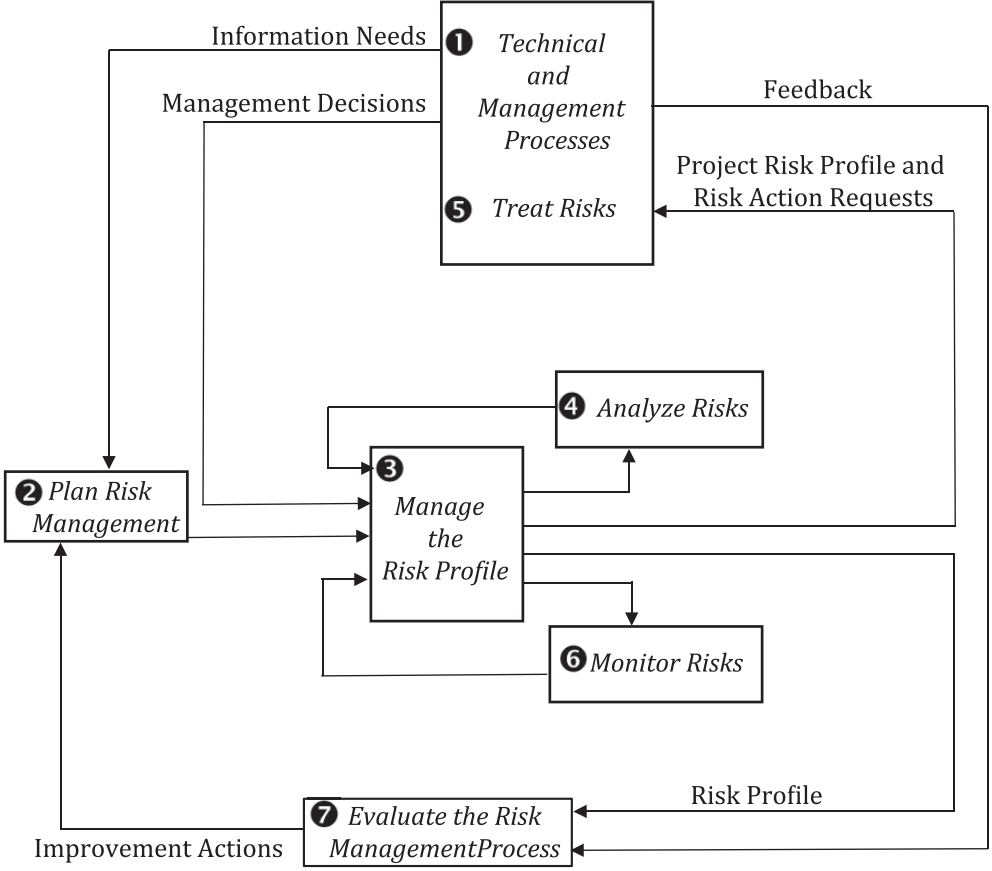
\includegraphics[width=0.8\textwidth]{modelo-processo-gerenciamento-riscos}
	\legend{Fonte: \citeonline{iso16085}}
\end{figure}

Os \textbf{Processos técnicos e de gestão} que envolvem as partes interessadas definem os requisitos de informação (ou seja, as informações que as partes interessadas precisam para tomar decisões informadas envolvendo riscos) que apoiam o processo de gerenciamento de riscos. Esses requisitos de informação são repassados tanto para as atividades de Planejamento da gestão de riscos quanto para Gerenciamento do perfil de risco.

Na atividade de \textbf{Planejamento da gestão de riscos}, são definidas as políticas relativas às diretrizes gerais sob as quais o gerenciamento de riscos será conduzido, os procedimentos a serem usados, as técnicas específicas a serem aplicadas e outros assuntos relevantes ao planejamento de riscos. As informações criadas durante essa atividade devem ser documentadas em um plano de gerenciamento de riscos.

Na atividade de \textbf{Gerenciamento do perfil de risco}, são capturadas as informações sobre o contexto atual e histórico do gerenciamento de riscos e o estado dos riscos. O perfil de risco inclui o total de todos os perfis de risco individuais (ou seja, as informações atuais e históricas sobre um risco individual), que, por sua vez, inclui todos os estados de risco.

As informações do perfil de risco são continuamente atualizadas e mantidas por meio da atividade de \textbf{Análise de riscos}, que identifica os riscos, determina suas probabilidades e consequências, determina suas exposições ao risco e recomenda tratamentos para os riscos considerados acima dos seus limiares de risco. 

As recomendações de \textbf{Tratamento de riscos}, juntamente com o \textit{status} de outros riscos e seus \textit{status} de tratamento, são enviadas para a revisão da gerência. A gerência decide qual tratamento de risco será implementado para qualquer risco considerado inaceitável. Planos de tratamento de risco são criados para riscos que necessitam de tratamento. Esses planos são coordenados com outros planos de gerenciamento e outras atividades em andamento. As informações criadas durante essa atividade devem ser documentadas em um plano de tratamento de riscos.

Todos os riscos são continuamente monitorados até que não precisem mais ser rastreados, por exemplo, quando são eliminados, durante a atividade de \textbf{Monitoramento de riscos}. Além disso, novos riscos e fontes de risco são procurados. O processo de gerenciamento de riscos é avaliado para melhorar sua eficácia. Durante a atividade de \textbf{Avaliação do processo de gestão de riscos}, são capturadas informações, incluindo \textit{feedback} de usuários e outras partes, para melhorar o processo ou a capacidade da organização ou do projeto de gerenciar riscos. Melhorias definidas como resultado da avaliação são implementadas na atividade de Planejamento da gestão de riscos.

O processo de gerenciamento de riscos é aplicado continuamente ao longo do ciclo de vida do produto e é integrado com os outros processos do ciclo de vida. As atividades e tarefas do processo de gerenciamento de riscos interagem com os riscos individuais de maneira iterativa uma vez que o processo de gerenciamento de riscos começa. Por exemplo, na atividade de Análise de riscos, um risco pode ser reavaliado várias vezes durante a realização da avaliação de risco devido ao aumento do conhecimento sobre o risco obtido durante a própria tarefa de avaliação. O processo de gerenciamento de riscos não é um processo que segue de uma fase para a próxima, mas sim um processo iterativo e incremental que é implementado conforme necessário.

%------------------------------------------------------------------------------%

\subsubsection{Modelo do \textit{Software} Engineering Institute (CMMI)}

\citeonline{wazlawick2019} em Engenharia de \textit{Software} apresenta o modelo de gerenciamento de riscos do \textit{Software} Engineering Institute (SEI) e caracteriza da seguinte forma suas seis atividades:

\begin{enumerate}
  \item \textbf{Identificação}: antes que os riscos possam ser tratados, eles precisam ser identificados.
  \item \textbf{Análise}: transforma a lista de riscos potenciais em um documento mais útil para o planejador e o gerente de um projeto, pois, a partir dela, os riscos são priorizados, e o planejador e o gerente podem se concentrar nos riscos mais importantes sem perder tempo com os insignificantes.
  \item \textbf{Planejamento}: o planejamento quanto aos riscos permite ao gerente prevenir problemas, em geral de três formas:
  \begin{enumerate}
    \item planejando e executando planos para reduzir a probabilidade de o risco ocorrer;
    \item planejando e executando planos para reduzir o impacto do risco, caso ocorra;
    \item planejando as atividades de recuperação de projeto, caso o risco efetivamente tenha ocorrido.
  \end{enumerate}
  \item \textbf{Rastreamento}: o rastreamento (ou monitoramento) de riscos consiste em avaliar, ao longo do projeto, as propriedades do risco (por exemplo, a probabilidade de ele ocorrer). O rastreamento deve ser baseado em métricas de avaliação de risco.
  \item \textbf{Controle}: em função de mudanças no \textit{status} de um risco, alguns planos podem ter que ser executados. Muitas vezes, talvez seja necessário improvisar a resposta ao problema causado pelo risco.
  \item \textbf{Comunicação}: a comunicação é um processo fundamental ao longo de um projeto de \textit{software}, especialmente em relação à prevenção e ao tratamento de riscos. Assim, não há uma atividade específica de comunicação em riscos, pois se trata de uma prática que permeia todas as outras atividades.
\end{enumerate}

%------------------------------------------------------------------------------%

\subsubsection{Modelo do PMBOK}

O PMBOK \cite{PMBOK} possui um dos processos de gerenciamento de riscos mais conhecidos da área atualmente. Ele é definido em 7 etapas distintas:

\begin{enumerate}
  \item \textbf{Planejar o Gerenciamento dos Riscos}: Processo de definição de como conduzir as atividades de gerenciamento dos riscos de um projeto.

  O principal benefício deste processo é garantir que o grau, o tipo e a visibilidade do gerenciamento dos riscos sejam proporcionais tanto aos riscos como à importância do projeto para a organização e para as outras partes interessadas.
  
  Deve começar na concepção do projeto e estar concluído no início do projeto. Talvez seja necessário revisitar este processo mais tarde no ciclo de vida do projeto, por exemplo, em uma mudança importante de fase ou se houver mudança significativa no escopo do projeto ou se uma revisão subsequente da eficácia do gerenciamento dos riscos determinar que o processo de Gerenciamento dos Riscos do Projeto exige modificação.

  \item \textbf{Identificar os Riscos}: Processo de identificação dos riscos individuais do projeto, bem como fontes de risco geral do projeto, e de documentar suas características.
  
  O principal benefício deste processo é a documentação de cada risco de projeto existente e as fontes gerais de riscos do projeto. Também reúne informações para que a equipe do projeto possa responder de forma apropriada aos riscos identificados.
  
  Todas as partes interessadas do projeto devem ser incentivadas a identificar os riscos individuais do projeto. É especialmente importante envolver a equipe do projeto de modo que ela possa desenvolver e manter um sentido de propriedade e responsabilidade pelos riscos individuais identificados, o nível do risco geral do projeto e as respectivas ações de resposta aos riscos.

  Na descrição e registro de cada risco do projeto, deve-se usar um formato uniforme para as especificações dos riscos para garantir que cada risco seja compreendido claramente e sem equívocos.

  Identificar os riscos é um processo iterativo, pois novos riscos podem surgir no decorrer do projeto, através de seu ciclo de vida e o nível de risco geral do projeto também pode mudar.

  \item \textbf{Realizar a Análise Qualitativa dos Riscos}: Processo de priorização de riscos individuais do projeto para análise ou ação posterior, através da avaliação de sua probabilidade de ocorrência e impacto, assim como outras características.
  
  O principal benefício deste processo é que concentra os esforços em riscos de alta prioridade. Este processo é realizado ao longo do projeto.
  
  Este processo avalia a prioridade dos riscos individuais identificados do projeto utilizando as respectivas probabilidades de ocorrência e o impacto correspondente sobre os objetivos do projeto se os riscos ocorrerem e outros fatores. Essas avaliações são subjetivas, pois baseiam-se em percepções do risco pela equipe do projeto e outras partes interessadas. Portanto, uma avaliação eficaz requer a identificação explícita e o gerenciamento das atitudes dos riscos dos participantes chave no processo. A percepção do risco introduz a parcialidade na avaliação dos riscos identificados; por isso, é preciso estar atento para identificá-los e corrigi- los. Uma avaliação da qualidade das informações disponíveis sobre os riscos individuais do projeto também ajuda a esclarecer a avaliação da importância de cada risco para o projeto.

  \item \textbf{Realizar a Análise Quantitativa dos Riscos}: O processo de analisar numericamente o efeito combinado dos riscos individuais identificados no projeto e outras fontes de incerteza nos objetivos gerais do projeto.
  
  O principal benefício deste processo é que quantifica a exposição ao risco geral do projeto, e também pode fornecer informações quantitativas adicionais dos riscos para apoio do planejamento de respostas aos mesmos. Este processo não é necessário para todos os projetos.
  
  Realizar uma análise robusta depende da disponibilidade de dados de alta qualidade sobre os riscos individuais do projeto e outras fontes de incerteza, bem como uma sólida linha de base subjacente do projeto para escopo, cronograma e custo. A análise quantitativa dos riscos geralmente requer \textit{software} especializado e expertise no desenvolvimento e na interpretação dos modelos de riscos. O uso da análise quantitativa de riscos de um projeto será especificado no plano de gerenciamento dos riscos do projeto.

  \item \textbf{Planejar as Respostas aos Riscos}: O processo de desenvolver alternativas, selecionar estratégias e acordar ações para lidar com a exposição geral de riscos, e também tratar os riscos individuais do projeto.
  
  O principal benefício deste processo é que identifica formas apropriadas de abordar o risco geral e os riscos individuais do projeto. Este processo também aloca recursos e adiciona atividades em documentos do projeto e no plano de gerenciamento do projeto, conforme necessário.
  
  As respostas efetivas e apropriadas ao risco podem minimizar ameaças individuais, maximizar oportunidades individuais e reduzir a exposição geral ao risco do projeto. Respostas inadequadas ao risco podem ter o efeito inverso. As respostas planejadas devem ser adequadas à relevância do risco, ter eficácia de custos para atender ao desafio, serem realistas dentro do contexto do projeto, acordados por todas as partes envolvidas e ter um responsável designado.  
  
  Para cada risco, deve-se selecionar a estratégia ou a mescla de estratégias com maior probabilidade de eficácia. Um plano de contingência pode ser desenvolvido para implementação, caso a estratégia selecionada se mostre ineficaz, em parte, ou caso ocorra um risco aceito.

  \item \textbf{Implementar Respostas a Riscos}: Processo de implementar planos acordados de resposta aos riscos.
  
  O principal benefício deste processo é a garantia de que as respostas acordadas aos riscos sejam executadas conforme planejado a fim de abordar a exposição ao risco geral do projeto, minimizar ameaças individuais e maximizar as oportunidades individuais do projeto. Devida atenção a este processo garante que respostas acordadas são realmente executadas, pois um problema comum com o Gerenciamento dos Riscos é que as equipes empenhem esforços para identificar e analisar riscos e desenvolver respostas, mas nenhuma providência seja tomada para gerenciar os riscos.

  \item \textbf{Monitorar os Riscos}: Processo de monitorar a implementação de planos acordados de resposta aos riscos, acompanhar riscos identificados, identificar e analisar novos riscos, e avaliar a eficácia do processo de risco ao longo do projeto.
  
  O principal benefício deste processo é que habilita decisões do projeto com base em informações atuais sobre a exposição geral de risco e riscos individuais do projeto.
  
  Para garantir que a equipe do projeto e as partes interessadas chave estejam cientes do nível atual de exposição ao risco, o trabalho de projeto deve ser constantemente monitorado quanto a riscos individuais novos, alterados, defasados e para as mudanças no nível do risco geral do projeto pela aplicação do processo.
\end{enumerate}

%------------------------------------------------------------------------------%

\section{Métodos ágeis}

O modelo cascata começou a ser definido nos anos 1970 e é considerado o precursor de todos os ciclos de vida de \textit{software}. Baseado na filosofia \textit{Big Design Up Front}, ele propõe que antes de qualquer codificação é necessário realizar um trabalho detalhado de análise e design. O modelo é definido por documentação, determinando se as fases foram concluídas através de revisões ao final de cada uma das etapas \cite{wazlawick2019}. Apesar de sua abordagem estruturada, o modelo enfrenta desafios como a dificuldade de avaliar a qualidade e os riscos do projeto durante o desenvolvimento e a rigidez em lidar com mudanças nos requisitos, pontos que, como apontado por Wazlawick, tornam seu uso impraticável para muitos projetos reais.

Os desafios enfrentados por este modelo preditivo deram origem a ciclos de vida iterativos e incrementais, que abordam melhor as incertezas e as necessidades de adaptação ao longo do projeto. Diferentemente dos métodos preditivos, que se baseiam em planos detalhados para antecipar todas as etapas de um projeto, os métodos iterativos dividem o trabalho em ciclos menores, permitindo revisões frequentes e maior flexibilidade para ajustes \cite{AgileGuide}. Essa abordagem adaptativa é essencial em contextos de alta complexidade e incerteza, onde mudanças nos requisitos são inevitáveis.

No entanto, a principal distinção entre os métodos baseados em planos e os ágeis está no foco. Enquanto os métodos preditivos priorizam o cumprimento do plano inicial, os métodos ágeis enfatizam a entrega contínua de valor ao cliente e a resposta rápida a mudanças. Essa filosofia promove ciclos curtos de desenvolvimento, colaboração constante entre as partes interessadas e \textit{feedback} contínuo para ajustes ao produto final \cite{AgileGuide}.

A relevância dos métodos ágeis cresceu exponencialmente à medida que organizações perceberam as limitações do modelo preditivo em projetos dinâmicos e complexos. Com a ênfase na adaptação e entrega de valor, os métodos ágeis ganharam destaque em um ambiente onde a velocidade de resposta e a qualidade da entrega são fundamentais para atender às expectativas do mercado e dos clientes.

Em 2001 um grupo de 17 profissionais de \textit{software} se reuniu em Snowbird, Utah, para discutir formas de melhorar o desenvolvimento de \textit{software}. Dessa reunião surgiu o Manifesto Ágil, que delineia quatro valores fundamentais e doze princípios que promovem uma abordagem responsiva ao desenvolvimento de \textit{software} \cite{AgileManifest}. Os quatro valores centrais do Manifesto Ágil são:

\begin{itemize}
  \item Indivíduos e interações mais que processos e ferramentas.
  \item \textit{Software} funcionando mais que documentação abrangente.
  \item Colaboração com o cliente mais que negociação de contratos.
  \item Responder a mudanças mais que seguir um plano.
\end{itemize}
  
Os princípios do Manifesto enfatizam a entrega contínua de \textit{software} funcional, a aceitação de mudanças nos requisitos, a colaboração diária entre desenvolvedores e clientes, e a importância de equipes auto-organizadas e motivadas \cite{AgileManifest}. Os doze princípios do Manifesto são:
\begin{itemize}
  \item Nossa maior prioridade é satisfazer o cliente através da entrega contínua e adiantada de \textit{software} com valor agregado.
  \item Mudanças nos requisitos são bem-vindas, mesmo tardiamente no desenvolvimento. Processos ágeis tiram vantagem das mudanças visando vantagem competitiva para o cliente.
  \item Entregar frequentemente \textit{software} funcionando, de poucas semanas a poucos meses, com preferência à menor escala de tempo.
  \item Pessoas de negócio e desenvolvedores devem trabalhar diariamente em conjunto por todo o projeto.
  \item Construa projetos em torno de indivíduos motivados. Dê a eles o ambiente e o suporte necessário e confie neles para fazer o trabalho.
  \item O método mais eficiente e eficaz de transmitir informações para e entre uma equipe de desenvolvimento é através de conversa face a face.
  \item \textit{Software} funcionando é a medida primária de progresso.
  \item Os processos ágeis promovem desenvolvimento sustentável. Os patrocinadores, desenvolvedores e usuários devem ser capazes de manter um ritmo constante indefinidamente.
  \item Contínua atenção à excelência técnica e bom design aumenta a agilidade.
  \item Simplicidade \- a arte de maximizar a quantidade de trabalho não realizado \- é essencial.
  \item As melhores arquiteturas, requisitos e designs emergem de equipes auto-organizáveis.
  \item Em intervalos regulares, a equipe reflete sobre como se tornar mais eficaz e então refina e ajusta seu comportamento de acordo.
\end{itemize}

É levantado no \textit{Agile Practice Guide} \cite{AgileGuide} uma série de diferentes modelos ágeis existentes, cobrindo frameworks, métodos e práticas. Estes são destacados na Figura abaixo.

\begin{figure}[H]
  \centering
	\caption{\label{metodos-ageis}Métodos ágeis}
  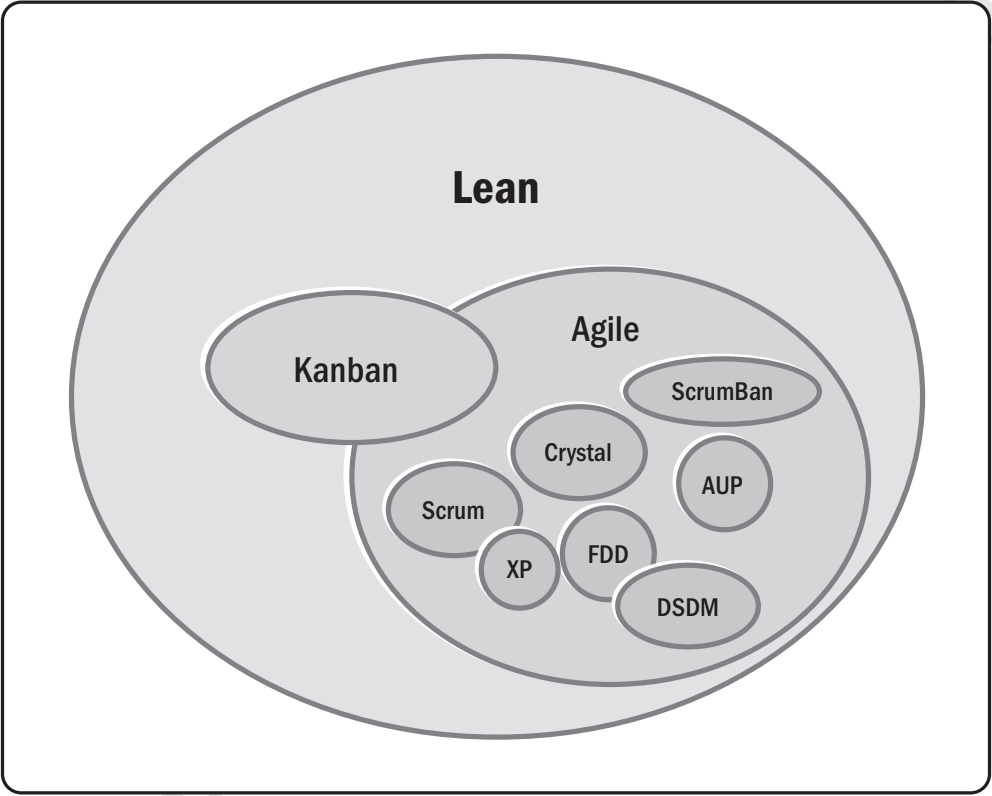
\includegraphics[width=0.6\textwidth]{metodos-ageis}
	\legend{Fonte: \textit{Agile Practice Guide} \cite{AgileGuide}}
\end{figure}

O \textit{Lean} é definido em \textit{Lean Software Development: An Agile Toolkit} \cite{Poppendieck_Poppendieck_2003} como uma abordagem que visa otimizar processos eliminando desperdícios e adicionando valor de acordo com a percepção do cliente. Entre seus princípios estão a eliminação de desperdícios, que envolve identificar e remover qualquer atividade que não agregue valor ao produto final. Amplificar o aprendizado é essencial, pois o desenvolvimento é um processo de descoberta contínua. Decidir o mais tarde possível permite tomar decisões mais informadas e com base em fatos concretos. A entrega rápida é fundamental para obter \textit{feedback} contínuo e atender rapidamente às necessidades dos clientes. A equipe deve ser empoderada para tomar decisões técnicas detalhadas, pois eles possuem o conhecimento mais profundo sobre o trabalho. Construir integridade no produto significa assegurar que ele atenda às expectativas do usuário e se mantenha útil ao longo do tempo. Finalmente, ver o todo é crucial para garantir que todas as partes do sistema trabalhem de forma coesa e otimizada, evitando a subotimização de componentes individuais.

\begin{figure}[H]
  \centering
	\caption{\label{annual-agile-report}\textit{Frameworks} utilizados pelos respondentes do \textit{Agile Report}}
  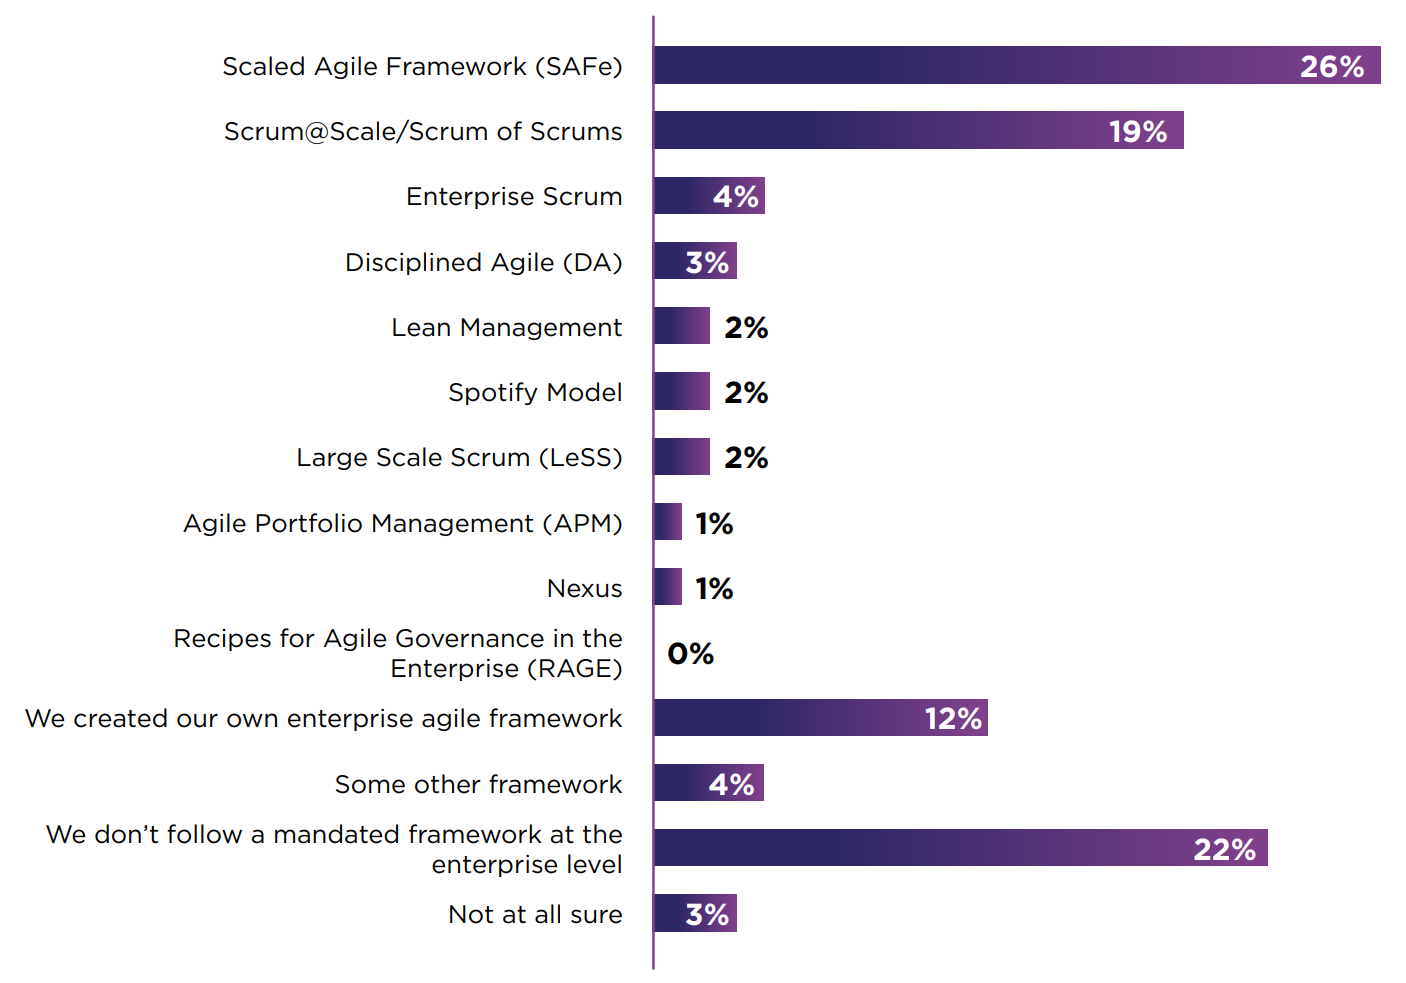
\includegraphics[width=0.8\textwidth]{annual-agile-report}
	\legend{Fonte: \textit{17th State of Agile Report} \cite{17_agile_report}}
\end{figure}

Como pode ser observado na Figura \ref{annual-agile-report}, segundo o \textit{17th State of Agile Report} \cite{17_agile_report}, entre os métodos ágeis mais utilizados em 2023 estão o \textit{Scrum} e o \textit{Scaled Agile Framework} (SAFe), definidos como:
\begin{itemize}
  \item \textbf{Scrum}: método ágil de gerenciamento de projetos que visa aumentar a produtividade das equipes de desenvolvimento. Ele não é um processo prescritivo, mas sim um \textit{framework} que se baseia em três pilares principais: transparência, inspeção e adaptação. A transparência assegura que todos os aspectos importantes do projeto sejam visíveis para os interessados, permitindo que clientes acompanhem o progresso e que desenvolvedores entendam claramente as necessidades do cliente. A inspeção envolve a revisão constante do trabalho realizado para garantir a qualidade e corrigir possíveis desvios. A adaptação permite que o processo de desenvolvimento evolua à medida que novos requisitos são descobertos ou atualizados \cite{wazlawick2019}.
  \item \textbf{\textit{Scaled Agile Framework} (SAFe)}: \textit{framework} ágil que visa escalar o desenvolvimento ágil em todos os níveis de uma organização, proporcionando uma base de conhecimento para padrões de trabalho. Baseado em princípios como pensamento sistêmico e preservação de opções em cenários variáveis, o SAFe incentiva a construção incremental com ciclos de aprendizado rápidos e integrados. Adicionalmente, prioriza a limitação de trabalho em progresso, sincronização de planejamento entre domínios e descentralização das tomadas de decisão. Sua abordagem foca em detalhar práticas, papéis e atividades em níveis de portfólio, programa e equipe, organizando a empresa em torno de fluxos de valor contínuo para o cliente \cite{AgileGuide}.
\end{itemize}

Apesar das diferenças, \textit{Scrum} e SAFe compartilham características comuns, como a ênfase na colaboração contínua com o cliente, a entrega frequente de valor em incrementos, a capacidade de adaptação a mudanças e a promoção de equipes auto-organizadas e multifuncionais. Ambos os frameworks incentivam o aprendizado contínuo, a transparência no trabalho e o alinhamento entre as partes interessadas, criando um ambiente que melhora a eficiência, a qualidade e a capacidade de atender às demandas dinâmicas do mercado.

%------------------------------------------------------------------------------%

\subsection{Gestão de riscos em métodos ágeis}

O gerenciamento de riscos em métodos ágeis segue uma abordagem que integra práticas e princípios fundamentais ao processo de desenvolvimento de \textit{software} inerentemente, sem que haja nenhum procedimento específico para a gestão de riscos \cite{Gold}. Práticas como retrospectivas, dailies e \textit{sprints} com entregas incrementais desempenham papel fundamental na identificação e mitigação de riscos, que acontecem de forma implícita. Essa forma implícita ocorre porque o processo ágil favorece ciclos curtos de \textit{feedback}, transparência e colaboração contínua entre as partes interessadas, o que permite identificar problemas ou ameaças de forma rápida e iterativa. Assim, os riscos são tratados à medida que surgem, promovendo ajustes frequentes ao longo do projeto.

Em outra perspectiva pode-se considerar que mesmo com o aumento da importância do gerenciamento de riscos entre as organizações, o gerenciamento de riscos tem sido negligenciado ou parcialmente suportado em métodos ágeis, já que os riscos podem surgir ao longo do ciclo de vida do projeto e não existe nenhuma ação específica para evitá-los \cite{LopesSamueldeSouza2022ARMF}. Pensando na prática, o \textit{Scrum}, por exemplo, tem uma seção para quaisquer “impedimentos” do projeto, que são ocorrências que possam impedir a equipe de funcionar de maneira eficaz. Do ponto de vista do gerenciamento de riscos, os impedimentos do projeto são problemas, riscos que ocorreram \cite{Gold}. Havendo um processo estruturado de gestão de riscos, não seria necessário tratar o problema, pois o risco que o gera poderia ter sido identificado e resolvido, antes de se tornar um problema.

\citeonline{LopesSamueldeSouza2022ARMF} vêem que devido à receptividade às mudanças no método ágil, vários projetos apresentam incertezas e riscos, e no formato atual, vários riscos permanecem desconhecidos porque são ignorados ao longo do ciclo de vida do projeto. Estes riscos podem ser gerenciados por meio de processos tradicionais de gerenciamento de riscos, desde que sejam adaptados ao contexto do desenvolvimento ágil.

Na pesquisa de \citeonline{Gold} foram identificados certos fatores que aumentam a eficácia do gerenciamento de riscos, um deles é a aplicação de um \textit{framework} de gerenciamento de riscos (identificação ágil de riscos, avaliação ágil de riscos, resposta ágil a riscos, revisão e monitoramento ágeis de riscos). Foi visto pelos entrevistados que a aplicação dessas etapas de gerenciamento de riscos tem grande influência positiva nos resultados do projeto, mostrando que o uso das práticas de gerenciamento de riscos neste cenário proporcionam resultados mais benéficos do que limitações. Foram avaliados os seguintes benefícios da aplicação do gerenciamento de riscos a projetos \textit{Scrum} \cite{Gold}:
\begin{itemize}
  \item Riscos e problemas ocorrem durante os projetos; uma equipe pode escolher ser reativa ou proativa em relação a esses riscos e problemas. O gerenciamento proativo de riscos durante todo o projeto é significativo para o sucesso do projeto e influencia positivamente o resultado do projeto.
  \item O gerenciamento de riscos ajuda a fornecer uma visão geral dos possíveis riscos que podem ser encontrados durante um projeto e a se preparar adequadamente para esses riscos.
  \item Embora o \textit{Scrum} já seja orientado a riscos devido à sua natureza ágil, a aplicação de um processo de gerenciamento de riscos reforça ainda mais esse método, melhorando sua entrega em relação aos seus fatores críticos de sucesso de tempo, custo e qualidade.
\end{itemize}

%------------------------------------------------------------------------------%

\section{Gamificação}

Definida como a aplicação de elementos de design de jogos fora do contexto de jogos, a gamificação visa aumentar o engajamento, a motivação e, consequentemente, os resultados dos indivíduos na atividade gamificada \cite{GARCIA201721}. Segundo \citeonline{Fardo_2013}, “a gamificação é um fenômeno com muitas potencialidades, pois a linguagem e metodologia dos games são bastante populares, eficazes na resolução de problemas [...] e aceitas naturalmente pelas atuais gerações.”, mostrando a gamificação como uma estratégia importante a ser explorada.

Aplicações da gamificação são amplas e variadas. Na educação, como observado por \citeonline{Alomari}, a gamificação pode transformar ambientes de aprendizagem ao tornar o estudo mais interativo e motivador. No marketing, ela pode aumentar a fidelidade dos clientes e a interação com a marca. No campo da saúde, a gamificação pode incentivar comportamentos saudáveis, como a prática de exercícios físicos e a adesão a tratamentos médicos. Ainda, como visto por \citeonline{Caponetto}, o uso da gamificação se mostra eficaz para alcançar objetivos transversais, como promover abordagens participativas e a colaboração entre pares, incentivar o aprendizado autodirigido e explorar a criatividade.

A gamificação envolve um processo de definição do ponto de vista de um designer de jogos, transformando uma tarefa em uma experiência que concentre o foco do participante para a resolução de um problema \cite{Fardo_2013}. Ela é criada a partir da integração de elementos comuns nos jogos, que, como identificado por \citeonline{Alomari}, podem envolver: sistemas de pontuação, badges, rankeamento (leaderboard), níveis, recompensas, barras de progresso, desafios, \textit{feedback} e avatares. \citeonline{Alomari} identifica os elementos típicos abaixo como as mais usadas e as caracteriza da seguinte forma:
\begin{itemize}
  \item \textbf{Points}: Pontos são definidos como valores numéricos que representam uma avaliação do indivíduo. Esta técnica fornece um \textit{feedback} sobre o progresso do indivíduo e pode aumentar a sua motivação.

  \item \textbf{Badges}: Badges são um maneira visual de representar as conquistas alcançadas pelo indivíduo na atividade. Assim como os pontos, ela impacta positivamente a motivação. Esta representação visual tem ênfase em melhorar a performance dos participantes.

  \item \textbf{Leaderboard}: Leaderboard são uma exibição do ranking dos participantes. Ele permite que o participante veja sua performance e a de seus colegas, o que resulta em um estímulo individual para engajar mais na atividade.
\end{itemize}

Pode ser observado na Figura \ref{duolingo} um exemplo do uso da técnica PBL (Points, Badges, Leaderboard) no aplicativo para aprendizado de línguas Duolingo.

\begin{figure}[H]
  \centering
	\caption{\label{duolingo}Sistema PBL no Duolingo}
  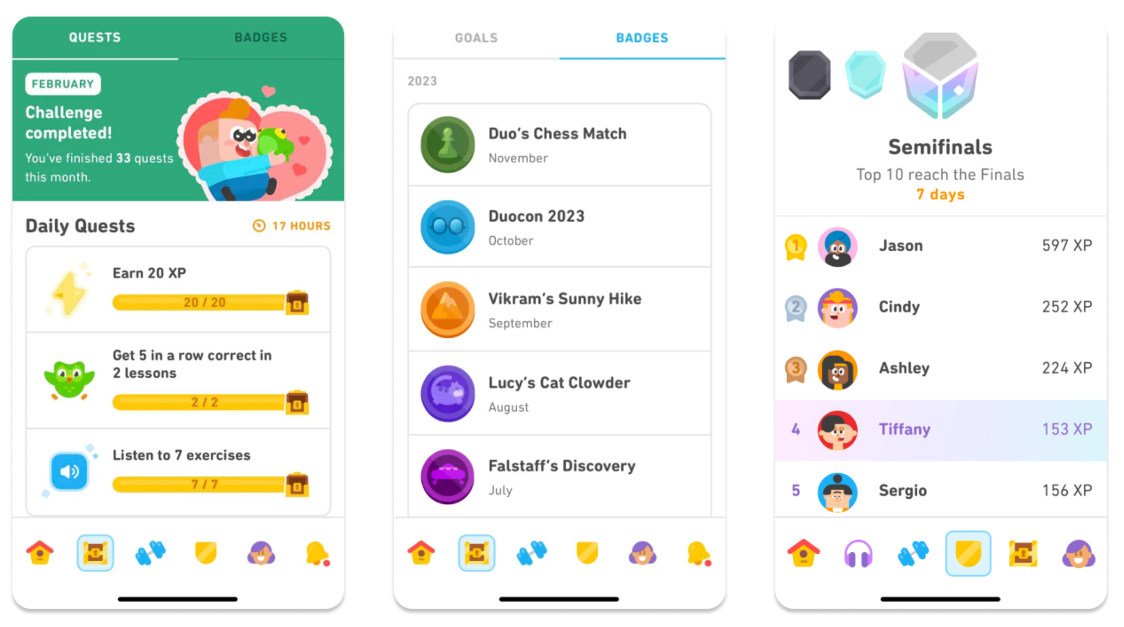
\includegraphics[width=0.8\textwidth]{duolingo}
	\legend{Fonte: Duolingo, Inc.}
\end{figure}

Para poder então criar um processo gamificado para uma atividade, \citeonline{GARCIA201721} identificam uma sequência bem definida de passos:

\renewcommand{\arraystretch}{1.3}

\begin{table}[h!]
  \caption{Metodologia para desenvolvimento de sistemas gamificados}
  \centering
  \resizebox{\textwidth}{!}{
  \begin{tabular}{|p{9cm}|p{6cm}|}
  \hline
  \textbf{Atividade} & \textbf{Descrição} \\ \hline
  \textbf{Identificação dos objetivos da gamificação} \newline 
  Tarefas: \newline 
  1.1 Definir o cenário atual \newline 
  1.2 Definir o cenário-alvo \newline 
  1.3 Estabelecer a missão SMART 
  & Os objetivos do programa de gamificação são definidos, juntamente com os indicadores correspondentes que devem avaliar o cumprimento dos objetivos. \\ \hline

  \textbf{Análise dos jogadores} \newline 
  Tarefas: \newline 
  2.1 Identificar a cultura organizacional e tipos de jogadores \newline 
  2.2 Coletar informações demográficas e psicográficas de todos os jogadores e adicionar isso ao perfil. 
  & Cada jogador é analisado em seu contexto para alinhar os perfis dos jogadores com os objetivos da gamificação. \\ \hline

  \textbf{Definição do escopo da gamificação e estudo de viabilidade} \newline 
  Tarefas: \newline 
  3.1 Estabelecer o escopo, motivadores, tipo de jogo (colaborativo, competitivo, individual) e diferentes possíveis soluções. \newline 
  3.2 Conduzir análise de viabilidade para cada alternativa e escolher a solução. 
  & Para definir o escopo da gamificação (cobertura do ciclo de vida do \textit{software} e motivadores intrínsecos/extrínsecos do jogo) e conduzir um estudo de viabilidade (econômica, técnica, operacional e legal), para escolher a melhor solução. \\ \hline

  \textbf{Análise e design do jogo} \newline 
  Tarefas: \newline 
  4.1 Escolher os componentes do jogo \newline 
  4.2 Escolher as mecânicas do jogo \newline 
  4.3 Estabelecer a economia do jogo \newline 
  4.4 Estabelecer a dinâmica do jogo (regras) \newline 
  4.5 Estabelecer a estética do jogo \newline 
  4.6 Elaborar os casos de uso do jogo 
  & O principal resultado desta atividade é o conjunto de requisitos (casos de uso do jogo) da ferramenta de \textit{software} em que o jogo está, e automatiza o jogo e seus elementos. \\ \hline

  \textbf{Desenvolvimento da plataforma gamificada} \newline 
  Tarefas para cada \textit{sprint}: \newline 
  5.1 Gestão da \textit{Sprint} \newline 
  5.2 Desenvolvimento da \textit{Sprint} (Preparação, Desenvolvimento, Teste) 
  & Desenvolvimento de \textit{software} da plataforma gamificada para SE a partir dos casos de uso do jogo. \\ \hline

  \textbf{Gerenciamento, monitoramento e medição} \newline 
  Tarefas: \newline 
  6.1 Coletar valores dos indicadores a partir dos logs de execução \newline 
  6.2 Analisar os indicadores e avaliar o cumprimento dos objetivos de negócios \newline 
  6.3 Desenvolver planos de ação para melhorar o sistema gamificado 
  & A plataforma gamificada é periodicamente monitorada para analisar o desempenho e o alcance dos objetivos de negócios. Quando são detectados desvios, planos de ação são desenvolvidos para refinar ou incluir no jogo os elementos necessários (componentes, mecânicas, dinâmica, estética). \\ \hline
  \end{tabular}
  }
  \label{tab:gamificacao}
  \legend{Fonte: Adaptado de \cite{GARCIA201721}}
\end{table}

%------------------------------------------------------------------------------%

\chapter{Estado da arte}
\label{cap:estado-arte}

A fim de levantar o estado da arte, foi realizada uma replicação e atualização do de Mapeamento Sistemático de Literatura (MSL) conduzido por \citeonline{garcia2023agreed} em seu trabalho de mestrad. Nesta replicação as diferenças foram a realização da análise apenas de estudos publicados a partir de 2021, período posterior ao do mapeamento original, e a não aplicação da técnica de Snowballing no ciclo final.

Assim como no mapeamento original, o MSL foi desenvolvido com o objetivo de analisar a integração de práticas explícitas de gestão de risco em métodos ágeis. Para isso, foram seguidos os procedimentos definidos por \citeonline{PETERSEN20151} e \citeonline{Petersen}, garantindo a aplicação de uma abordagem sistemática e rigorosa na condução da pesquisa.

\section{Protocolo de pesquisa}

A questão geral de pesquisa foi definida como: “Como as organizações de \textit{software} integram práticas explícitas de gerenciamento de riscos em métodos ágeis?” e esta foi dividida em quatro questões de análise detalhada, conforme apresentada na tabela abaixo.

\begin{table}[h!]
  \caption{Perguntas de pesquisa do MSL}
  \centering
  \begin{tabular}{|c|p{10cm}|}
  \hline
  \textbf{Pergunta} & \textbf{Descrição} \\ \hline
  Q1 & Qual contexto de uso de práticas de gestão de riscos nos métodos ágeis? \\ \hline
  Q2 & Quais práticas de gestão de riscos são introduzidas nos métodos ágeis? \\ \hline
  Q3 & Quais tipos de riscos são gerenciados? \\ \hline
  Q4 & Quais os resultados da introdução de práticas explícitas de gestão de riscos nos métodos ágeis? \\ \hline
  \end{tabular}
  \label{tab:perguntas-msl}
  \legend{Fonte: \citeonline{garcia2023agreed}}
\end{table}

A Tabela~\ref{tab:picoc} \cite{kitchenham2007guidelines} mostra os critérios e o escopo da estrutura da pergunta de pesquisa, que é a estrutura de População, Intervenção, Comparação, Resultados e Contexto (PICOC).

\begin{table}[H]
  \centering
  \caption{Descrição dos elementos PICOC da Pesquisa}
  \begin{tabular}{|p{3cm}|p{12cm}|}
  \hline
  \textbf{Critérios} & \textbf{Descrição} \\ \hline
  População \newline Intervenção \newline Comparação \newline Resultado \newline Contexto 
  & Organizações de \textit{software} \newline Aplicação da gerência de riscos \newline Não se aplica (N/A) \newline Se a qualidade do produto, prazo de entrega, etc foram impactados \newline Utilização de métodos ágeis \\ \hline
  \end{tabular}
  \label{tab:picoc}
  \legend{Fonte: \citeonline{garcia2023agreed}}
\end{table}

% A comparação é definida como “N/A” por se tratar de um mapeamento sistemático.

%------------------------------------------------------------------------------%

\subsection{String de busca e fontes de pesquisa}

A string de busca foi aplicada nas bibliotecas digitais IEEEXplore, ACM Digital Library e Scopus, devido à sua relevância para a área de engenharia de \textit{software}. A string de busca foi adaptada à sintaxe específica de cada biblioteca e aplicada aos campos de título e resumos. A pesquisa foi realizada em setembro de 2024.

\begin{table}[h!]
  \centering
  \begin{tabular}{|p{15cm}|}
  \hline
  “risk” AND (“agile” OR “scrum” OR “xp” OR “extreme programming” OR “lean” OR “kanban” OR “scrumban” OR “fdd” OR “feature driven development” OR “crystal” OR “iterative development”) AND “software” \\ \hline
  \end{tabular}
  \label{tab:consulta-pesquisa}
  \legend{Fonte: \citeonline{garcia2023agreed}}
\end{table}

As adaptações específicas da string de pesquisa para cada biblioteca digital estão disponíveis no \hyperref[apendiceA]{Apêndice A}.

%------------------------------------------------------------------------------%

\section{Critérios de inclusão e exclusão}

Com base na questão de pesquisa principal, os seguintes critérios de inclusão e exclusão foram definidos. Para além do estudo original, o critério de inclusão 4 foi adicionado, para o mapeamento de apenas estudos publicados após o fim do mapeamento original.

\begin{table}[H]
  \centering
  \caption{Critérios de inclusão}
  \begin{tabular}{|c|l|}
  \hline
  \textbf{Critério} & \textbf{Descrição} \\ \hline
  IC1 & Estudos primários revisados por pares \\ \hline
  IC2 & Escrito em inglês \\ \hline
  IC3 & Trabalhos completos com pelo menos 4 páginas \\ \hline
  IC4 & Trabalhos publicado a partir de 2021 \\ \hline
  \end{tabular}
  \legend{Fonte: Adaptado de \cite{garcia2023agreed}}
\end{table}

\begin{table}[H]
  \centering
  \caption{Critérios de exclusão}
  \begin{tabular}{|c|l|}
  \hline
  \textbf{Critério} & \textbf{Descrição} \\ \hline
  EC1 & Trabalho/proposta teórica não aplicada empiricamente \\ \hline
  EC2 & Estudos duplicados \\ \hline
  EC3 & Texto completo indisponível \\ \hline
  EC4 & Não focado no desenvolvimento de \textit{software} \\ \hline
  \end{tabular}
  \legend{Fonte: \citeonline{garcia2023agreed}}
\end{table}

%------------------------------------------------------------------------------%

\section{Processo de seleção}

A seleção dos estudos foi realizada em três ciclos, conforme Figura \ref{numero-estudos-ciclo}.

\begin{figure}[H]
	\centering
  \caption{\label{numero-estudos-ciclo}Número de estudos por ciclo}
  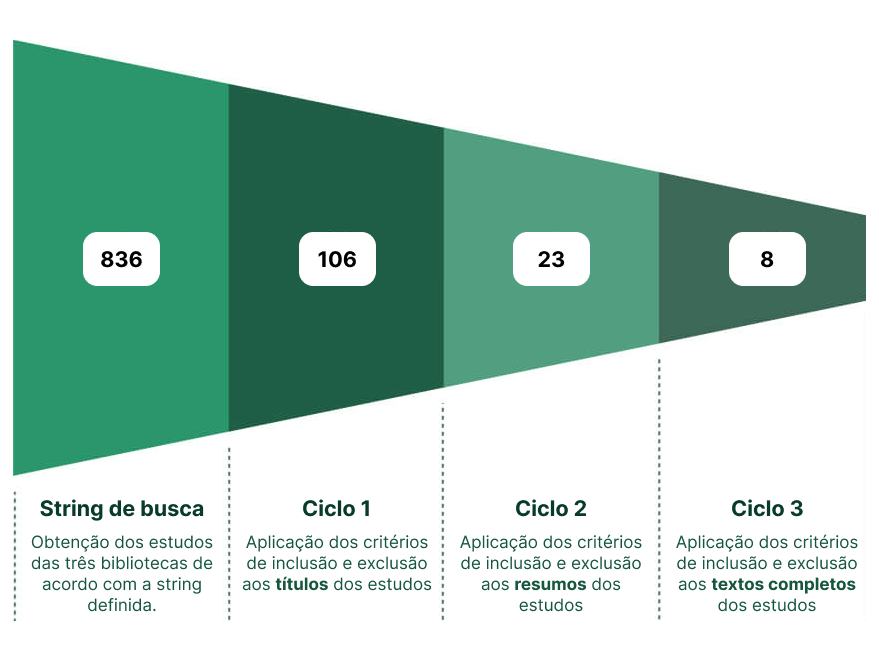
\includegraphics[width=0.7\textwidth]{numero-estudos-ciclo}
	\legend{Fonte: Autora (2024)}
\end{figure}

\begin{itemize}
  \item Para iniciar os ciclos, a string de busca foi aplicada às bibliotecas digitais, onde se obteve 836 estudos primários que foram submetidos à próxima etapa.
  \item No ciclo 1, a lista de estudos anterior foi submetida aos critérios de inclusão e exclusão em seus títulos e a nova seleção resultou em 106 estudos selecionados.
  \item No ciclo 2, a lista de estudos anterior foi submetida aos critérios de inclusão e exclusão em seus resumos e a nova seleção resultou em 23 estudos selecionados.
  \item No ciclo 3, a lista de estudos anterior foi submetida aos critérios de inclusão e exclusão em seus textos completos e esta última e final seleção resultou em 7 estudos selecionados.
\end{itemize}

\begin{table}[h!]
  \centering
  \caption{Resultados por biblioteca digital e ciclo}
  \begin{tabular}{|c|c|c|c|c|}
  \hline
  \textbf{Biblioteca} & \textbf{Total} & \textbf{Ciclo 1} & \textbf{Ciclo 2} & \textbf{Ciclo 3} \\ \hline
  ACM & 185 & 29 & 4 & 1 \\ \hline
  Scopus & 304 & 51 & 14 & 4 \\ \hline
  IEEE Xplore & 347 & 26 & 5 & 2 \\ \hline
  Todos & 836 & 106 & 23 & 7 \\ \hline
  \end{tabular}
  \legend{Fonte: Autora (2024)}
\end{table}

Os 7 estudos primários selecionados estão disponíveis no \hyperref[apendiceB]{Apêndice B}.

%------------------------------------------------------------------------------%

\section{Extração dos dados}

Os dados coletados dos estudos primários selecionados são apresentados e analisados de acordo com cada questão de análise pré-definida. Os dados brutos extraídos estão disponíveis em: \href{https://docs.google.com/spreadsheets/d/1YY_yjyBefJ3ZmnEY38TM_LnZLoJcKhrw_q0BdEvqx2E/edit?gid=1276800509#gid=1276800509}{MSL público}. Uma síntese do DEF está descrita na Tabela~\ref{sintese}.

\begin{table}[H]
  \centering
  \caption{Síntese do DEF}
  \begin{tabular}{|p{2.4cm}|c|p{9.5cm}|}
  \hline
  \textbf{Questão de pesquisa} & \textbf{Identificador} & \textbf{Descrição} \\ \hline
  Q1 & Q1.1 & Contexto de aplicação do estudo \\ \hline
  Q1 & Q1.2 & Método ágil utilizado/impactado \\ \hline
  Q1 & Q1.3 & Tipo de validação do estudo \\ \hline
  Q1 & Q1.4 & Número de projetos que o estudo foi aplicado \\ \hline
  Q2 & Q2.1 & Lista/descrição das práticas propostas \\ \hline
  Q2 & Q2.2 & Processo de gerenciamento de risco impactado pelas práticas propostas \\ \hline
  Q3 & Q3.1 & Riscos enfrentados nos projetos \\ \hline
  Q4 & Q4.1 & Síntese do resultado dos estudos empíricos \\ \hline
  \end{tabular}
  \label{sintese}
  \legend{Fonte: \cite{garcia2023agreed}}
\end{table}

\textbf{Q1. Qual é o contexto de uso das práticas de gestão de risco em métodos ágeis?}

Na Tabela~\ref{contexto} é possível observar a resposta direta de cada uma dos seccionamentos desta pergunta.

\begin{table}[h!]
  \centering
  \caption{Contexto de uso}
  \begin{tabular}{|c|l|l|}
  \hline
  \textbf{Questão} & \multicolumn{2}{c|}{\textbf{Extracted data}} \\ \hline
  \multirow{2}{*}{Q1.1 - Ambiente} & Indústria & S1, S2, S3, S5, S7 \\ \cline{2-3}
                                  & Academia  & S4, S6 \\ \hline
  \multirow{6}{*}{Q1.2 - Método ágil} & Scrum   & S2, S4 \\ \cline{2-3}
                                     & XP      & S2 \\ \cline{2-3}
                                     & DAD     & S5 \\ \cline{2-3}
                                     & SAFe    & S5 \\ \cline{2-3}
                                     & Não definido & S1, S3, S6, S7 \\ \hline
  \multirow{3}{*}{Q1.3 - Tipo}        & Estudo de caso & S2, S3, S5, S7 \\ \cline{2-3}
                                     & Experimento    & S1, S4 \\ \cline{2-3}
                                     & Survey         & S6 \\ \hline
  \multirow{2}{*}{Q1.4 - Instâncias}  & Exatamente 1   & S1, S2, S6, S7 \\ \cline{2-3}
                                     & Exatamente 2   & S3, S4, S5 \\ \hline
  \end{tabular}
  \label{contexto}
  \legend{Fonte: Autora (2024)}
  \end{table}

Os estudos selecionados foram conduzidos em dois ambientes distintos (Q2.1): indústria de \textit{software} e academia. Dos estudos analisados, 71\% foram realizados em organizações de desenvolvimento de \textit{software}, enquanto 29\% foram conduzidos em ambiente acadêmico.

Quanto aos métodos ágeis adotados (Q2.2), \textit{Scrum} foi mencionado em 2 estudos, XP, DAD e SAFe em 1 estudo cada. Além disso, de forma maior, 4 estudos não mencionaram nenhum método ágil específico.

Em relação ao tipo de estudo empírico (Q2.3), metade dos estudos utilizaram estudos de caso, 28\% realizaram experimentos e 14\% aplicaram surveys. Observa-se que, na indústria, predominam os estudos de caso, como observado no mapeamento original.
O número de projetos em que o estudo foi aplicado ficou entre apenas 1 e 2, divididos de forma semelhante, 57\% dos estudos aplicados em apenas 1 organização e 43\% aplicaram em 2 organizações.

\textbf{Q2. Quais práticas de gerenciamento de risco são introduzidas nos métodos ágeis?}

Assim como observado no mapeamento original, duas estratégias diferentes foram adotadas pelos estudos para integrar a gestão de riscos aos métodos ágeis: usar as práticas ágeis existentes ou introduzir novas práticas de gestão de riscos.

O estudo S5 adotou a primeira estratégia, em suas ações integrando a gestão de riscos a itens já existentes nos processos dos métodos ágeis. Adotando a segunda estratégia, os outros estudos primários criaram novas práticas ágeis ou introduziram práticas tradicionais adaptadas em métodos ágeis para melhorar o gerenciamento de riscos. Abaixo alguns exemplos de práticas são descritos.

Em S1 é instituído o RM3, que é composto por três processos principais: análise de complexidade do projeto, análise de riscos e monitoramento e controle de riscos. Onde em (1) utiliza-se a matriz de complexidade, uma ferramenta qualitativa para avaliar objetivamente os fatores de complexidade e seu impacto; (2) Análise de riscos: identifica todos os riscos, tanto negativos quanto positivos, com base nos pressupostos e restrições do projeto. Utiliza a exposição ao risco como medida quantitativa para avaliar e priorizar os riscos; (3) Monitoramento e controle de riscos: aplica ações de resposta ao risco e monitora os riscos identificados, atualizando-os conforme necessário. Este processo inclui monitorar e tratar riscos residuais, identificar novos riscos e avaliar a eficácia das respostas. Além disso, atualiza os ativos dos processos organizacionais, como modelos de gestão de riscos e lições aprendidas, beneficiando futuros projetos.

No estudo S2, um \textit{backlog} específico para riscos é adicionado aos produtos da metodologia para registrar e gerenciar todos os riscos identificados. Além das tarefas do \textit{scrum}, as tarefas de gestão de riscos em cada \textit{sprint} são realizadas em três passos: planejamento (identificar e registrar todos os riscos no \textit{backlog}), aplicação de estratégia (priorizar os riscos com base em fatores de prioridade, inserir os riscos de maior prioridade no ciclo de iteração do \textit{scrum}, e aplicar a estratégia apropriada para cada risco) e supervisão e controle (monitorar a eliminação dos riscos e assegurar que a estratégia está sendo eficaz). No final de cada \textit{sprint}, avalia-se a harmonia entre as estratégias aplicadas e os riscos. Caso novos riscos sejam identificados ou riscos existentes persistam, eles retornam ao \textit{backlog} de riscos para análise e tratamento em \textit{sprints} futuras.

Em S7, é descrito o problema de minimização de perdas por riscos no processo de design de \textit{software} definido considerando vetor de variáveis de decisão. Onde a partir da probabilidade de ocorrência do risco para o i-ésimo recurso, o valor das perdas por unidade do i-ésimo recurso associado à ocorrência do risco, o número do recurso do projeto é feito o cálculo da estimativa total de risco (R). E a função objetivo: determinar a quantidade de cada recurso a ser alocado no projeto, de forma que a função objetivo \(F(x)\) (o custo de compensação das consequências dos riscos) seja minimizada.

\textbf{Q3. Que tipos de riscos são gerenciados?}

Os estudos primários selecionados identificam um total de 97 riscos. Assim como no mapeamento original foram agrupados por meio da taxonomia de \citeonline{Taxonomy}, uma taxonomia de riscos que fornece três classes de riscos, seus elementos e atributos. Todos os riscos relatados nos estudos primários selecionados foram coletados, classificados de acordo com a taxonomia e resumidos no \hyperref[apendiceC]{Apêndice C}. A lista completa de riscos, suas fontes e as classificações escolhidas está disponível em: \href{https://docs.google.com/spreadsheets/d/1YY_yjyBefJ3ZmnEY38TM_LnZLoJcKhrw_q0BdEvqx2E/edit?usp=drivesdk}{link}.

Apenas 5 dos 7 estudos listaram de forma explícita os riscos enfrentados nos projetos. Deste grupo, o estudo primário que relatou o maior número de riscos foi S5, com um total de 63 riscos, tendo alta distribuição entre as diferentes classes, elementos e atributos, como é possível observar na Figura \ref{dist-contagem-classe-atributo}.

\begin{figure}[H]
  \centering
	\caption{\label{dist-contagem-classe-atributo}Distribuição de contagem por classe e atributo de S5}
  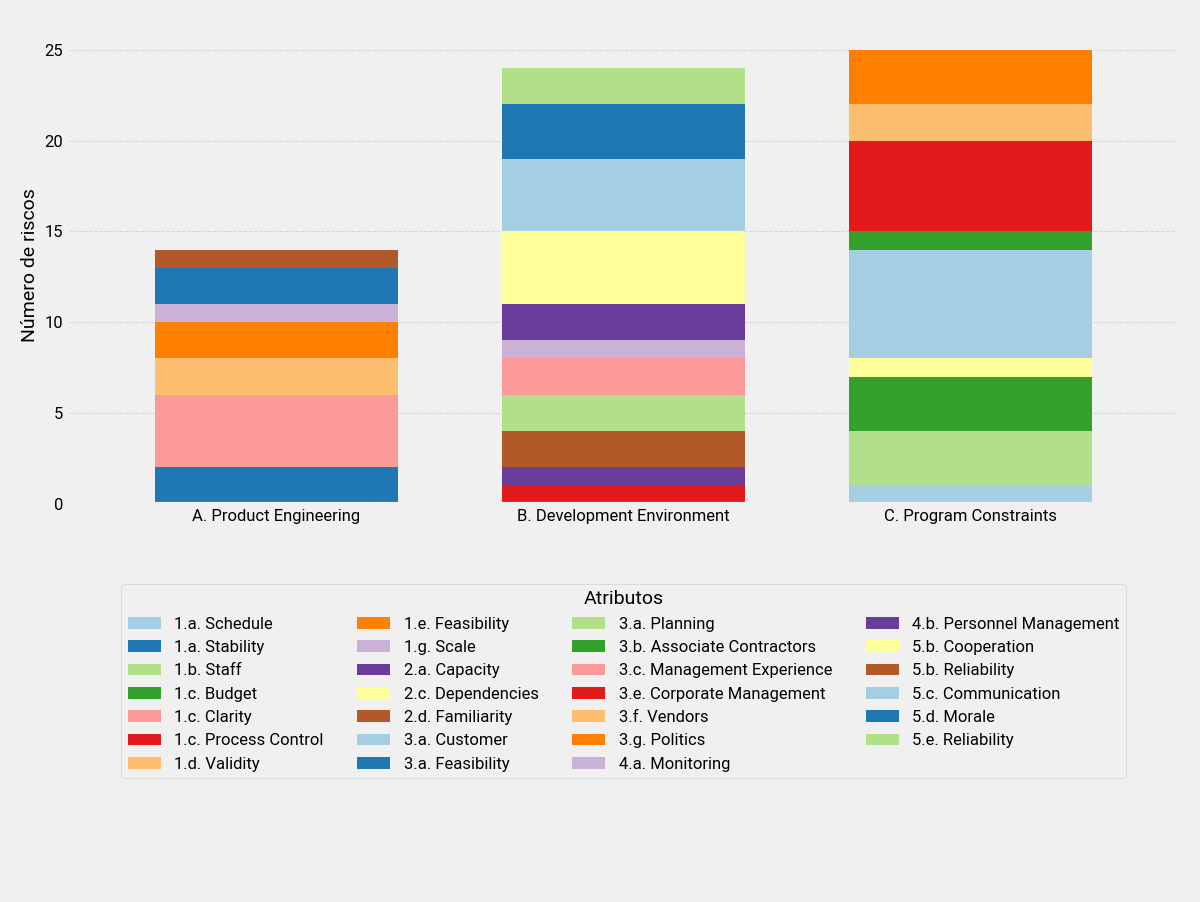
\includegraphics[width=0.9\textwidth]{dist-contagem-classe-atributo}
	\legend{Fonte: Autora (2024)}
\end{figure}

O atributo com maior frequência de riscos foram “\textit{Schedule}”, da classe “\textit{Program Constraints}”, identificado em 4 dos estudos primários. Em sequência “\textit{Staff}”, da classe “\textit{Product Engineering}”, “\textit{Communication}”, da classe “\textit{Development Environment}” e “\textit{Stability}”, “\textit{Clarity}”, “\textit{Validity}” e “\textit{Feasibility}”, da classe “\textit{Product Engineering}”, obtiveram 3 ocorrências cada.

O elemento com maior número de ocorrências de riscos foi “\textit{Resources}”, registrado em 4 estudos primários. “\textit{Product Engineering}” e “\textit{Program Constraints}” foram as classes que apresentaram o maior número de ocorrências, ambas com registros em 4 estudos.

\textbf{Q4. Quais são os resultados da introdução de práticas explícitas de gerenciamento de riscos em métodos ágeis?}

Todos os estudos selecionados relatam impactos positivos da introdução de práticas explícitas de gerenciamento de riscos, mas três estudos (43\%) [S2, S5, S7] destacaram explicitamente impactos positivos sem comprometer a agilidade dos métodos ágeis.

Em S1 do ponto de vista financeiro, de escopo e de prazos, o projeto foi bem-sucedido e atendeu às expectativas da equipe. Houve menos tempo gasto em atividades desnecessárias, o que permitiu mais foco e ausência de riscos inesperados. Os recursos foram liberados conforme planejado, garantindo a qualidade das entregas e continuidade do trabalho da equipe em outros projetos. Foi aplicado um questionário para medir a satisfação da equipe, do cliente e das partes interessadas com o uso do RM3, e o resultado foi muito positivo, demonstrando preferência pelo RM3 em relação ao método anterior.

No estudo S3, aplicado em projetos com mais de 5 mil horas de duração de 5 a 10 meses para serem concluídos, o uso do \textit{framework} gerou um aumento positivo na reação média aos riscos, com uma taxa de melhoria de cerca de 49\%.

Em S4 os resultados indicam um aumento significativo no conhecimento sobre gestão de riscos ao utilizar o jogo, destacando seu valor educacional e eficácia como ferramenta de apoio ao ensino. Houve uma melhoria de 85\% nas respostas do questionário do Grupo AAS, com apenas 15\% dos participantes mantendo as mesmas respostas iniciais.

Na análise de S5 o mapeamento teórico demonstra como os frameworks escaláveis de ágil — DAD e SAFe — podem potencialmente eliminar ou mitigar os riscos de projetos de \textit{software} no contexto de desenvolvimento global.

\section{Discussão}

Como também identificado no mapeamento original, a maioria dos estudos foram feitos na indústria, mostrando o potencial impacto positivo das ações de gestão de risco para esta área. Havendo também 50\% dos estudos relatando impactos positivos sem comprometer a agilidade dos métodos ágeis. Além disso, estudos de caso são predominantes na indústria, enquanto experimentos e surveys têm menor representatividade, mostrando uma tendência de abordagem empírica para avaliar os contextos de uso dessas práticas.

As práticas de gestão de riscos nos métodos ágeis se dividem em duas estratégias principais: o uso das práticas ágeis já existentes e a introdução de novas práticas adaptadas. Por exemplo, práticas como reuniões diárias e planejamento de \textit{sprints} foram aproveitadas para integrar a gestão de riscos, além da inclusão de uma reunião semanal dedicada a riscos. Por outro lado, foi observado também a ideia de criação de um \textit{backlog} específico para riscos, ou ainda do uso de métodos quantitativos para minimizar perdas, como o cálculo de estimativa total de risco e alocação de recursos.

Os tipos de riscos gerenciados foram classificados em uma grande variedade de atributos em todas as classes. Estudos como S5, que identificou 63 riscos, mostram a complexidade e a amplitude dos desafios enfrentados, destacando a necessidade de métodos estruturados e adaptados para lidar com essas incertezas no desenvolvimento ágil.

Por fim, os resultados indicam impactos positivos significativos na introdução de práticas explícitas de gestão de riscos, sem comprometer a agilidade dos métodos ágeis. Exemplos incluem a melhoria na eficiência e qualidade das entregas, maior conhecimento sobre gestão de riscos e aumento da eficácia no tratamento de riscos com ferramentas específicas, como Rm4Am. Esses resultados reforçam a relevância de integrar práticas de gestão de riscos aos métodos ágeis para alcançar maior sucesso nos projetos.


\subsection{Ameaças à validade}

As mesmas ameaças à validade avaliadas no mapeamento original também estão presentes nesta replicação, como o risco de buscas incompletas, a limitação no número de estudos analisados, a tendência de publicação de resultados positivos e a qualidade empírica limitada de muitos dos estudos incluídos. Ademais, a técnica de Snowballing não foi aplicada nesta replicação, o que impossibilitou a identificação de estudos adicionais e pode ter levado à omissão de trabalhos relevantes. Por fim, como este estudo é uma replicação, eventuais problemas não identificados na pesquisa original também foram reproduzidos, o que pode impactar os resultados e conclusões deste trabalho.


%------------------------------------------------------------------------------%
%------------------------------------------------------------------------------%

\chapter{Proposta}
\label{cap:proposta}

Seguindo o \textit{framework} de gamificação em engenharia de \textit{software} proposto por \citeonline{GARCIA201721}, nas seções seguintes são apresentadas as atividades realizadas para o desenvolvimento da dinâmica de gamificação voltada à identificação de riscos em contextos ágeis. O \textit{framework} prevê as seguintes etapas para essa definição:

\begin{enumerate}
  \item Identificação dos objetivos da gamificação;
  \item Análise dos participantes; 
  \item Definição do escopo da gamificação e estudo de viabilidade;
  \item Análise e design do jogo; 
  \item Desenvolvimento da plataforma gamificada;
  \item Gerenciamento, monitoramento e medição. 
\end{enumerate}

\section{Identificação dos objetivos da gamificação}

A primeira etapa do \textit{framework} busca estabelecer um conjunto de objetivos para a gamificação. Para isso, é necessário examinar o cenário atual e o desejado, identificando situações que podem ser aprimoradas por meio da gamificação e de que forma essas melhorias podem ocorrer. Por fim, os objetivos devem ser convertidos em metas SMART, que possibilitem a mensuração dos avanços.

\begin{enumerate}
  \item \textbf{Cenário atual}: Equipes ágeis atuam em modelos nos quais o gerenciamento de riscos é implícito, sem etapas estruturadas ou práticas específicas para a identificação e análise de riscos. Essa ausência pode levar à negligência de riscos potenciais, cuja concretização compromete o andamento dos projetos e a entrega de valor.
  
  \item \textbf{Cenário-alvo}: Implementar uma dinâmica gamificada que facilite a identificação e análise de riscos no contexto de equipes ágeis. A intenção é oferecer um espaço estruturado e colaborativo para que os membros da equipe reconheçam riscos potenciais e alinhem ações de mitigação, promovendo maior clareza e previsibilidade no trabalho, sem comprometer a agilidade dos processos.
  
  \item \textbf{Meta}: Desenvolver uma dinâmica gamificada que possibilite às equipes ágeis compreender melhor os riscos associados aos seus projetos e ampliar a percepção coletiva sobre possíveis impactos, promovendo uma análise mais estruturada e eficaz em pelo menos uma equipe piloto. A validação será feita por meio de \textit{feedback} qualitativo dos participantes, considerando a clareza e a aplicabilidade da abordagem.
\end{enumerate}

\section{Análise de participantes}

A segunda etapa enfatiza a importância de analisar os participantes para os quais se está projetando a solução, visando criar experiências que melhorem sua motivação e engajamento. Essa análise considera os jogadores como elemento central do ambiente, avaliando suas motivações, objetivos e interação com as mecânicas propostas. O processo envolve a identificação da cultura organizacional e dos perfis de participantes, que podem ser categorizados segundo taxonomias como a de \citeonline{Bartle}, além de dados psicográficos e demográficos.

No contexto brasileiro, segundo dados da \citeonline{jetbrains2023dev}, 51\% dos profissionais do setor de TI têm menos de 30 anos. Essa estatística é corroborada regionalmente pela pesquisa realizada em Santa Catarina \cite{acate}, que aponta uma média de idade em torno de 33 anos. O setor é majoritariamente masculino, com apenas 21,2\% de participação feminina, conforme dados da \citeonline{softex2023industriatic}. Em relação à formação acadêmica, mais de 85\% dos profissionais possuem graduação em áreas de tecnologia, com destaque para Sistemas de Informação, Análise e Desenvolvimento de Sistemas, Ciências da Computação e Engenharia \cite{revelo2021tecnologia}.

Quanto às especialidades, 30,5\% dos profissionais se identificam como Full-stack, seguidos por Back-end (27,2\%) e Front-end (24,2\%) \cite{revelo2021tecnologia}. Os segmentos mais representativos de atuação são Serviços e Telecomunicações (25,9\%), Finanças (25,6\%) e Indústria (18,9\%) \cite{abes2023mercado}. Além disso, 63\% dos profissionais afirmam preferir o uso do \textit{Scrum} em nível de equipe, demonstrando a prevalência desse \textit{framework} entre as equipes ágeis \cite{17_agile_report}.

Como resumido na Tabela~\ref{tab:analise_usuario}, esses dados evidenciam um perfil majoritário de profissionais jovens, especializados em tecnologia e adaptados ao uso de metodologias ágeis, o que reforça a relevância de soluções gamificadas para esse público.

\begin{table}[H]
  \centering
  \caption{Análise de usuário}
  \label{tab:analise_usuario}
  \begin{tabular}{|p{8cm}|}
  \hline
  \textbf{Análise de usuário} \\ \hline
  Homem \\ \hline
  33 anos \\ \hline
  Full-stack \\ \hline
  Bacharel em Sistemas de Informação \\ \hline
  Atuação em Serviços e Telecomunicações \\ \hline
  Utilização de Scrum \\ \hline
  Categoria de Bartle: Achievers e Explorers \\ \hline
  \end{tabular}
  \legend{Fonte: Autora (2024)}
\end{table}

\section{Definição do escopo da gamificação e estudo de viabilidade}

Na terceira etapa, as informações obtidas nas análises anteriores permitem definir uma abordagem inicial para a solução gamificada. Primeiramente, é necessário delimitar o escopo da solução, identificando quais processos, tipos de usuários e ferramentas serão impactados, com base nos objetivos estabelecidos na primeira etapa. A partir dos dados sobre os participantes, coletados na segunda etapa, define-se o tipo de ambiente gamificado a ser criado, formulando alternativas iniciais para a solução. Por fim, é realizada a análise de viabilidade de cada alternativa proposta.

\subsection{Escopo, motivadores, tipo de jogo e possíveis soluções}

A dinâmica proposta tem como objetivo principal facilitar a identificação e análise de riscos em equipes ágeis, promovendo um ambiente mais interativo e colaborativo. Ao integrar elementos de gamificação ao processo de gerenciamento de riscos, espera-se engajar os participantes e fomentar uma compreensão mais profunda dos potenciais problemas que podem surgir durante os projetos.

Optou-se por um modelo predominantemente colaborativo, com possíveis elementos competitivos secundários. Essa escolha reflete melhor a realidade das equipes ágeis, nas quais o sucesso depende do esforço conjunto para superar desafios, e o trabalho multidisciplinar é valorizado. Esse formato também estimula a troca de ideias e o compartilhamento de diferentes perspectivas, enriquecendo o processo de identificação de riscos.

A dinâmica busca contemplar, principalmente, as etapas iniciais do gerenciamento de riscos, com foco na identificação e análise. Essas etapas foram escolhidas por representarem pontos críticos — e frequentemente negligenciados — em projetos conduzidos com métodos ágeis, devido à ausência de práticas explícitas para o tratamento de riscos. Essa lacuna favorece o surgimento de problemas inesperados, muitas vezes evitáveis por meio de uma identificação antecipada.

Foram idealizadas pela autora diversas alternativas de gamificação, descritas na Tabela~\ref{tab:dinamicas}.

\begin{longtable}{|p{3cm}|p{12cm}|}
  \caption{Dinâmicas de gestão de riscos idealizadas} \label{tab:dinamicas} \\ \hline
  \textbf{Nome} & \textbf{Descrição} \\ \hline
  \endfirsthead
  \hline
  \textbf{Nome} & \textbf{Descrição} \\ \hline
  \endhead
  \hline
  \multicolumn{2}{|c|}{\textit{Continua na próxima página}} \\ \hline
  \endfoot
  \hline
  \multicolumn{2}{|c|}{\textit{Fim da tabela}} \\ \hline
  \endlastfoot
  Tarot dos Riscos & Dinâmica inspirada no Tarot da Tecnologia. Os participantes utilizam um conjunto de cartas contendo diferentes cenários de risco. Cada carta é discutida em grupo, avaliando sua aplicação e relevância no contexto do projeto atual. O objetivo é promover a troca de ideias e alinhar percepções sobre os principais riscos. \\ \hline
  6 Chapéus & Adaptação da técnica dos \href{https://brasil.uxdesign.cc/escolhendo-ferramentas-six-thinking-hats-2e30da00ec9b}{6 chapéus}. Cada participante é designado com uma perspectiva diferente para mapear os riscos do projeto e sugerir resoluções iniciais. A estrutura promove uma análise abrangente dos problemas identificados. \\ \hline
  Crazy 8s & Adaptação da dinâmica de design \href{https://laboratoriobridge.github.io/bthinking/pt/methods/crazy8/}{Crazy 8s}. Cada participante lista oito riscos em até oito minutos, incentivando criatividade e agilidade. Em seguida, os riscos são compartilhados e analisados pela equipe. Participantes com listas inovadoras recebem prêmios simbólicos, promovendo engajamento e colaboração. \\ \hline
  Tapple & Baseado no jogo \href{https://ludopedia.com.br/jogo/tapple}{Tapple}, os participantes utilizam a mecânica pré-definida do jogo e listam um risco para cada letra disponível dentro do tempo limite. A dinâmica ocorre em rodadas rápidas, promovendo identificação e priorização ágil dos riscos. \\ \hline
  Amarelinha Game Board & Dinâmica inspirada no jogo da amarelinha. Cada participante apresenta um risco, e o grupo avalia sua probabilidade e impacto. O valor combinado determina o número de casas que o participante avança no tabuleiro. A atividade combina análise de risco com elementos lúdicos para engajamento. \\ \hline
  Baralho de Riscos em Matriz & Dinâmica baseada em cartas, onde cada uma representa um risco distinto. Os participantes compram cartas e categorizam os riscos em uma matriz de probabilidade e impacto. O objetivo é priorizar os riscos e promover uma análise estruturada. \\ \hline
  CPV & Dinâmica que utiliza um \textit{canvas} para categorizar e organizar os riscos. Os participantes preenchem seções específicas do \textit{canvas}, permitindo uma análise visual e estruturada dos principais riscos do projeto. \\ \hline
  Retrospectiva de Riscos & Adaptação da técnica de retrospectiva, com foco nos riscos enfrentados durante o projeto. A equipe revisa os riscos previamente identificados, avalia sua ocorrência e discute lições aprendidas para melhorar estratégias futuras de mitigação. \\ \hline
  Sequenciador & Baseada na técnica \href{https://caroli.org/sequenciador/}{Sequenciador}, de Paulo Caroli. Os participantes organizam os riscos identificados em diferentes níveis e, por fim, em uma sequência de prioridade. A dinâmica utiliza cartões e debates para promover alinhamento e priorização. \\ \hline
  \textit{Planning Poker} dos Riscos & Dinâmica que adapta o \textit{Planning Poker}. Os participantes utilizam cartas para votar sobre a probabilidade e impacto de cada risco. O consenso obtido nas rodadas serve para priorizar os riscos mais críticos. \\ \hline
  Poke Risk (Super Trunfo) & Dinâmica inspirada no universo Pokémon. Cada risco é representado por uma carta com parâmetros como probabilidade e impacto, definidos previamente pelos participantes. Durante o jogo, as cartas são comparadas em rodadas, priorizando os riscos com maior gravidade. A dinâmica combina elementos de cartas e \textit{board game} para análise colaborativa. \\ \hline
\end{longtable}
\legend{Fonte: Autora (2024)}

Em seguida, são apresentadas com mais detalhes as ideias priorizadas para refinamento.

\subsubsection{Tarot dos Riscos}

A proposta do Tarot dos Riscos é inspirada no \href{https://tarotcardsoftech.artefactgroup.com/}{\textit{The Tarot Cards of Tech}}, criado pela \textit{Artefact Group}. A dinâmica tem como objetivo apoiar a identificação de riscos por meio de cartas que representam diferentes categorias ou cenários. Cada carta apresenta uma breve descrição de um risco potencial, associado a situações comuns em projetos ágeis, como mudanças de requisitos, atrasos ou falhas de comunicação.

A atividade é realizada em equipe: os participantes sorteiam cartas e discutem como cada risco poderia impactar o projeto em questão, promovendo o pensamento crítico e a antecipação de problemas. Com base nas discussões, espera-se que a equipe avance posteriormente para a análise e mitigação dos riscos identificados.

\begin{itemize}
\item \textbf{Vantagens}: Incentiva o diálogo entre os membros da equipe e facilita o engajamento. A inclusão de exemplos concretos nas cartas auxilia na identificação de riscos que poderiam passar despercebidos. 
\item \textbf{Desvantagens}: Pode ser limitada em relação a riscos muito específicos que não estejam contemplados nas cartas existentes, dependendo fortemente da qualidade da curadoria inicial. Equipes menos colaborativas podem apresentar baixa adesão à dinâmica.
\end{itemize}

A simplicidade de criação e aplicação torna essa dinâmica bastante viável, especialmente em ambientes com tempo limitado para atividades. As cartas podem ser impressas ou disponibilizadas digitalmente.

\begin{figure}[H]
  \centering
  \caption{\label{tarot-da-tecnologia} \textit{The Tarot Cards of Tech}}
  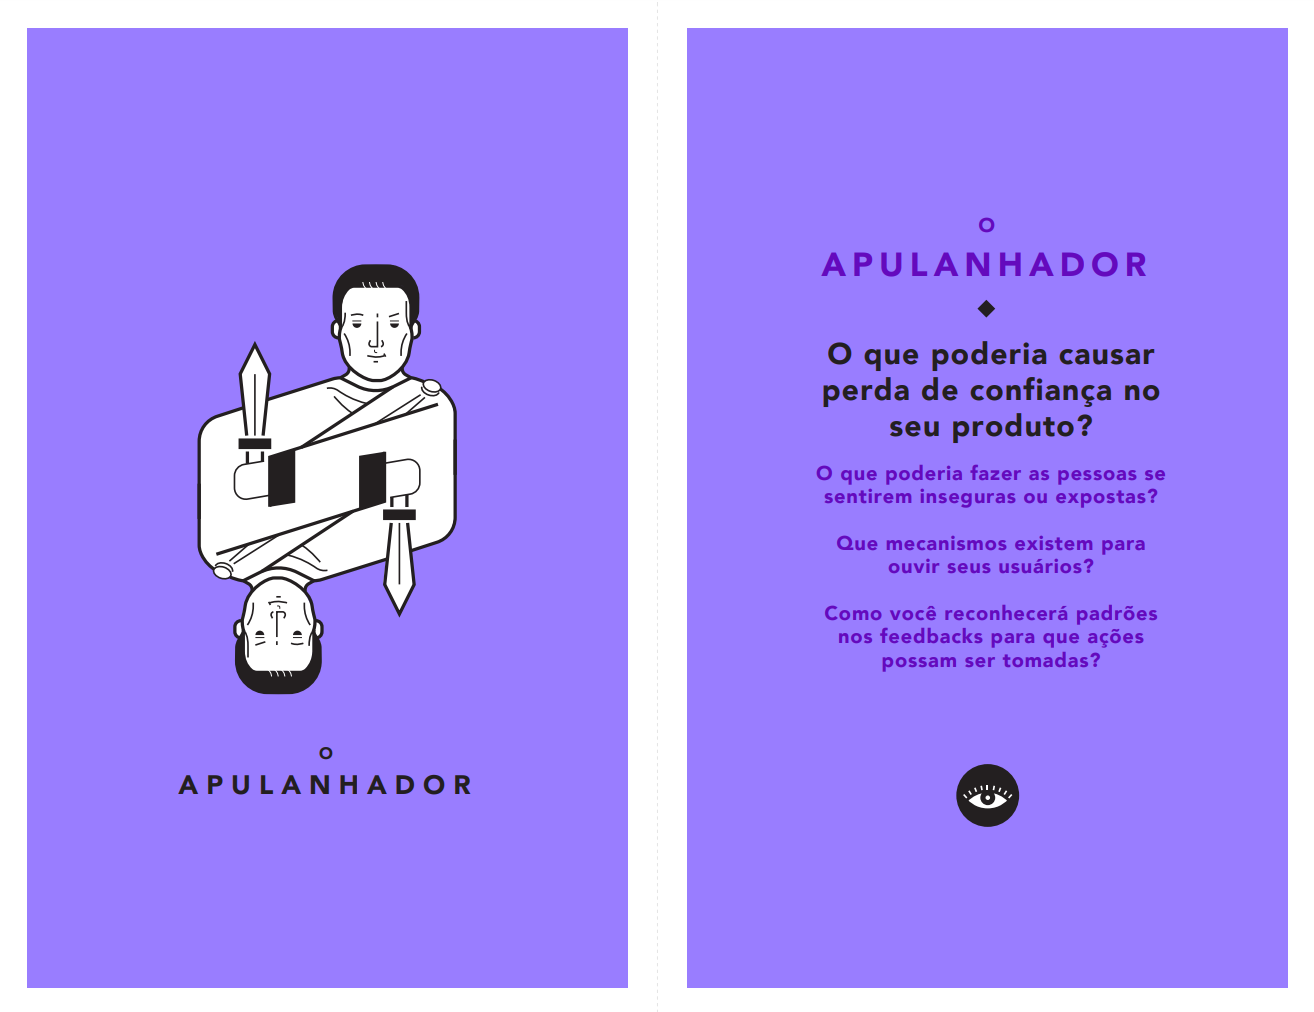
\includegraphics[width=0.65\textwidth]{tarot-da-tecnologia}
  \legend{Fonte: \href{https://www.artefactgroup.com/}{\textit{Artefact Group}}}
\end{figure}

\subsubsection{Amarelinha Game Board}

O Amarelinha Game Board combina gamificação e análise de riscos em uma dinâmica interativa. A atividade segue uma trilha no estilo da amarelinha, em que cada participante, em sua vez, anuncia um risco identificado. Após o anúncio, os demais participantes classificam o risco e calculam um valor com base em sua probabilidade e severidade. Esse valor define o número de casas que o participante avança no tabuleiro. O objetivo é alcançar o “céu” antes dos demais jogadores.

\begin{itemize}
  \item \textbf{Vantagens}: Promove tanto a identificação quanto a categorização dos riscos, ensinando de forma prática como avaliar probabilidade e impacto. O caráter lúdico e competitivo pode aumentar a motivação dos participantes. 
  \item \textbf{Desvantagens}: A competitividade pode desviar o foco em grupos onde o objetivo principal é a colaboração. A mecânica de cálculo pode ser desafiadora para equipes com pouca experiência em análise de riscos, sendo recomendável a mediação de um facilitador. 
\end{itemize}

Essa proposta apresenta viabilidade moderada. Requer preparação prévia para definição das categorias e montagem do tabuleiro, mas pode ser adaptada com recursos simples ou versões digitais.

\begin{figure}[H]
  \centering
  \caption{\label{amarelinha}Amarelinha caracol}
  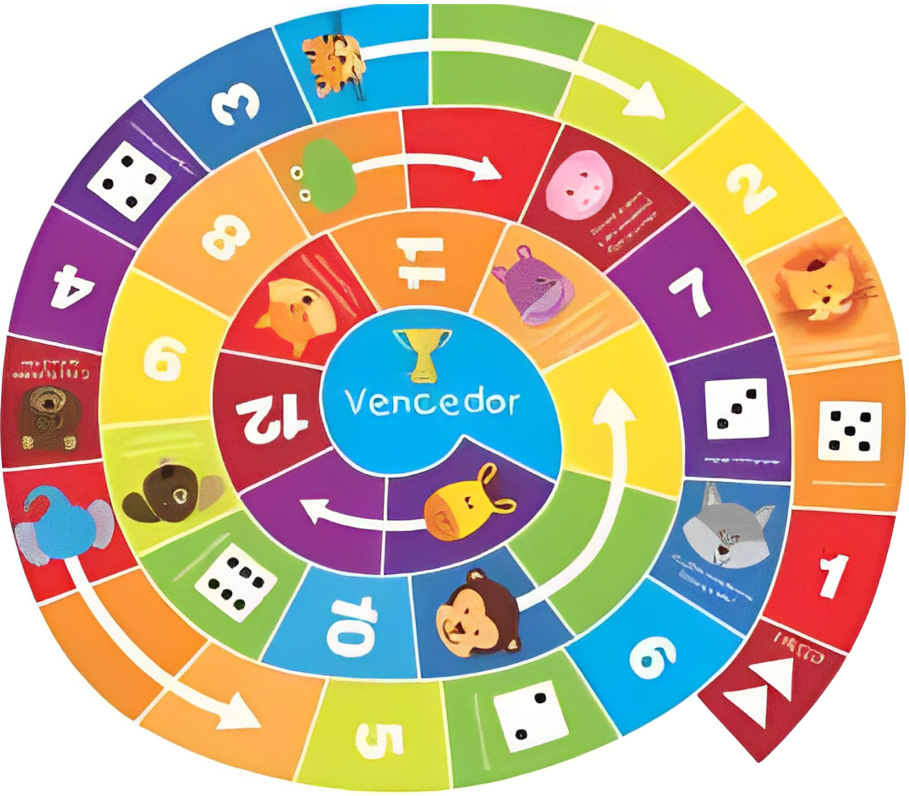
\includegraphics[width=0.6\textwidth]{amarelinha}
  \legend{Fonte: Ri Happy}
\end{figure}

\subsubsection{Poke Risk (Super Trunfo)}

O Poke Risk é uma dinâmica inspirada no universo dos jogos de Pokémon, em que cada carta representa um risco que a equipe pode enfrentar. Antes do início do jogo, os participantes preenchem as cartas com parâmetros como probabilidade, impacto e cenário do risco. Durante a atividade, essas cartas são utilizadas para promover discussão, análise e priorização.

Cada jogador compra cartas do monte principal até que todas tenham sido distribuídas. A seguir, os participantes enfrentam “batalhas de riscos”: em cada rodada, um jogador escolhe o atributo da sua carta com maior valor para tentar superar a carta do oponente. A carta vencedora integra um novo monte, que representa os riscos a serem priorizados na definição das estratégias de mitigação.

\begin{itemize}
  \item \textbf{Vantagens}: A abordagem lúdica torna a análise de riscos mais envolvente, especialmente para equipes que apreciam dinâmicas criativas e baseadas em jogos. 
  \item \textbf{Desvantagens}: Requer maior tempo de preparação e familiarização dos participantes com os conceitos de análise de risco. Sem um facilitador experiente, a atividade pode perder o foco ou se tornar menos produtiva. 
\end{itemize}

Essa proposta também apresenta viabilidade moderada. A criação inicial das cartas exige tempo e alinhamento prévio, mas pode ser realizada de forma colaborativa pela equipe, assegurando a relevância dos riscos representados.

\begin{figure}[H]
  \centering
  \caption{\label{super-trunfo}Super Trunfo Pokémon}
  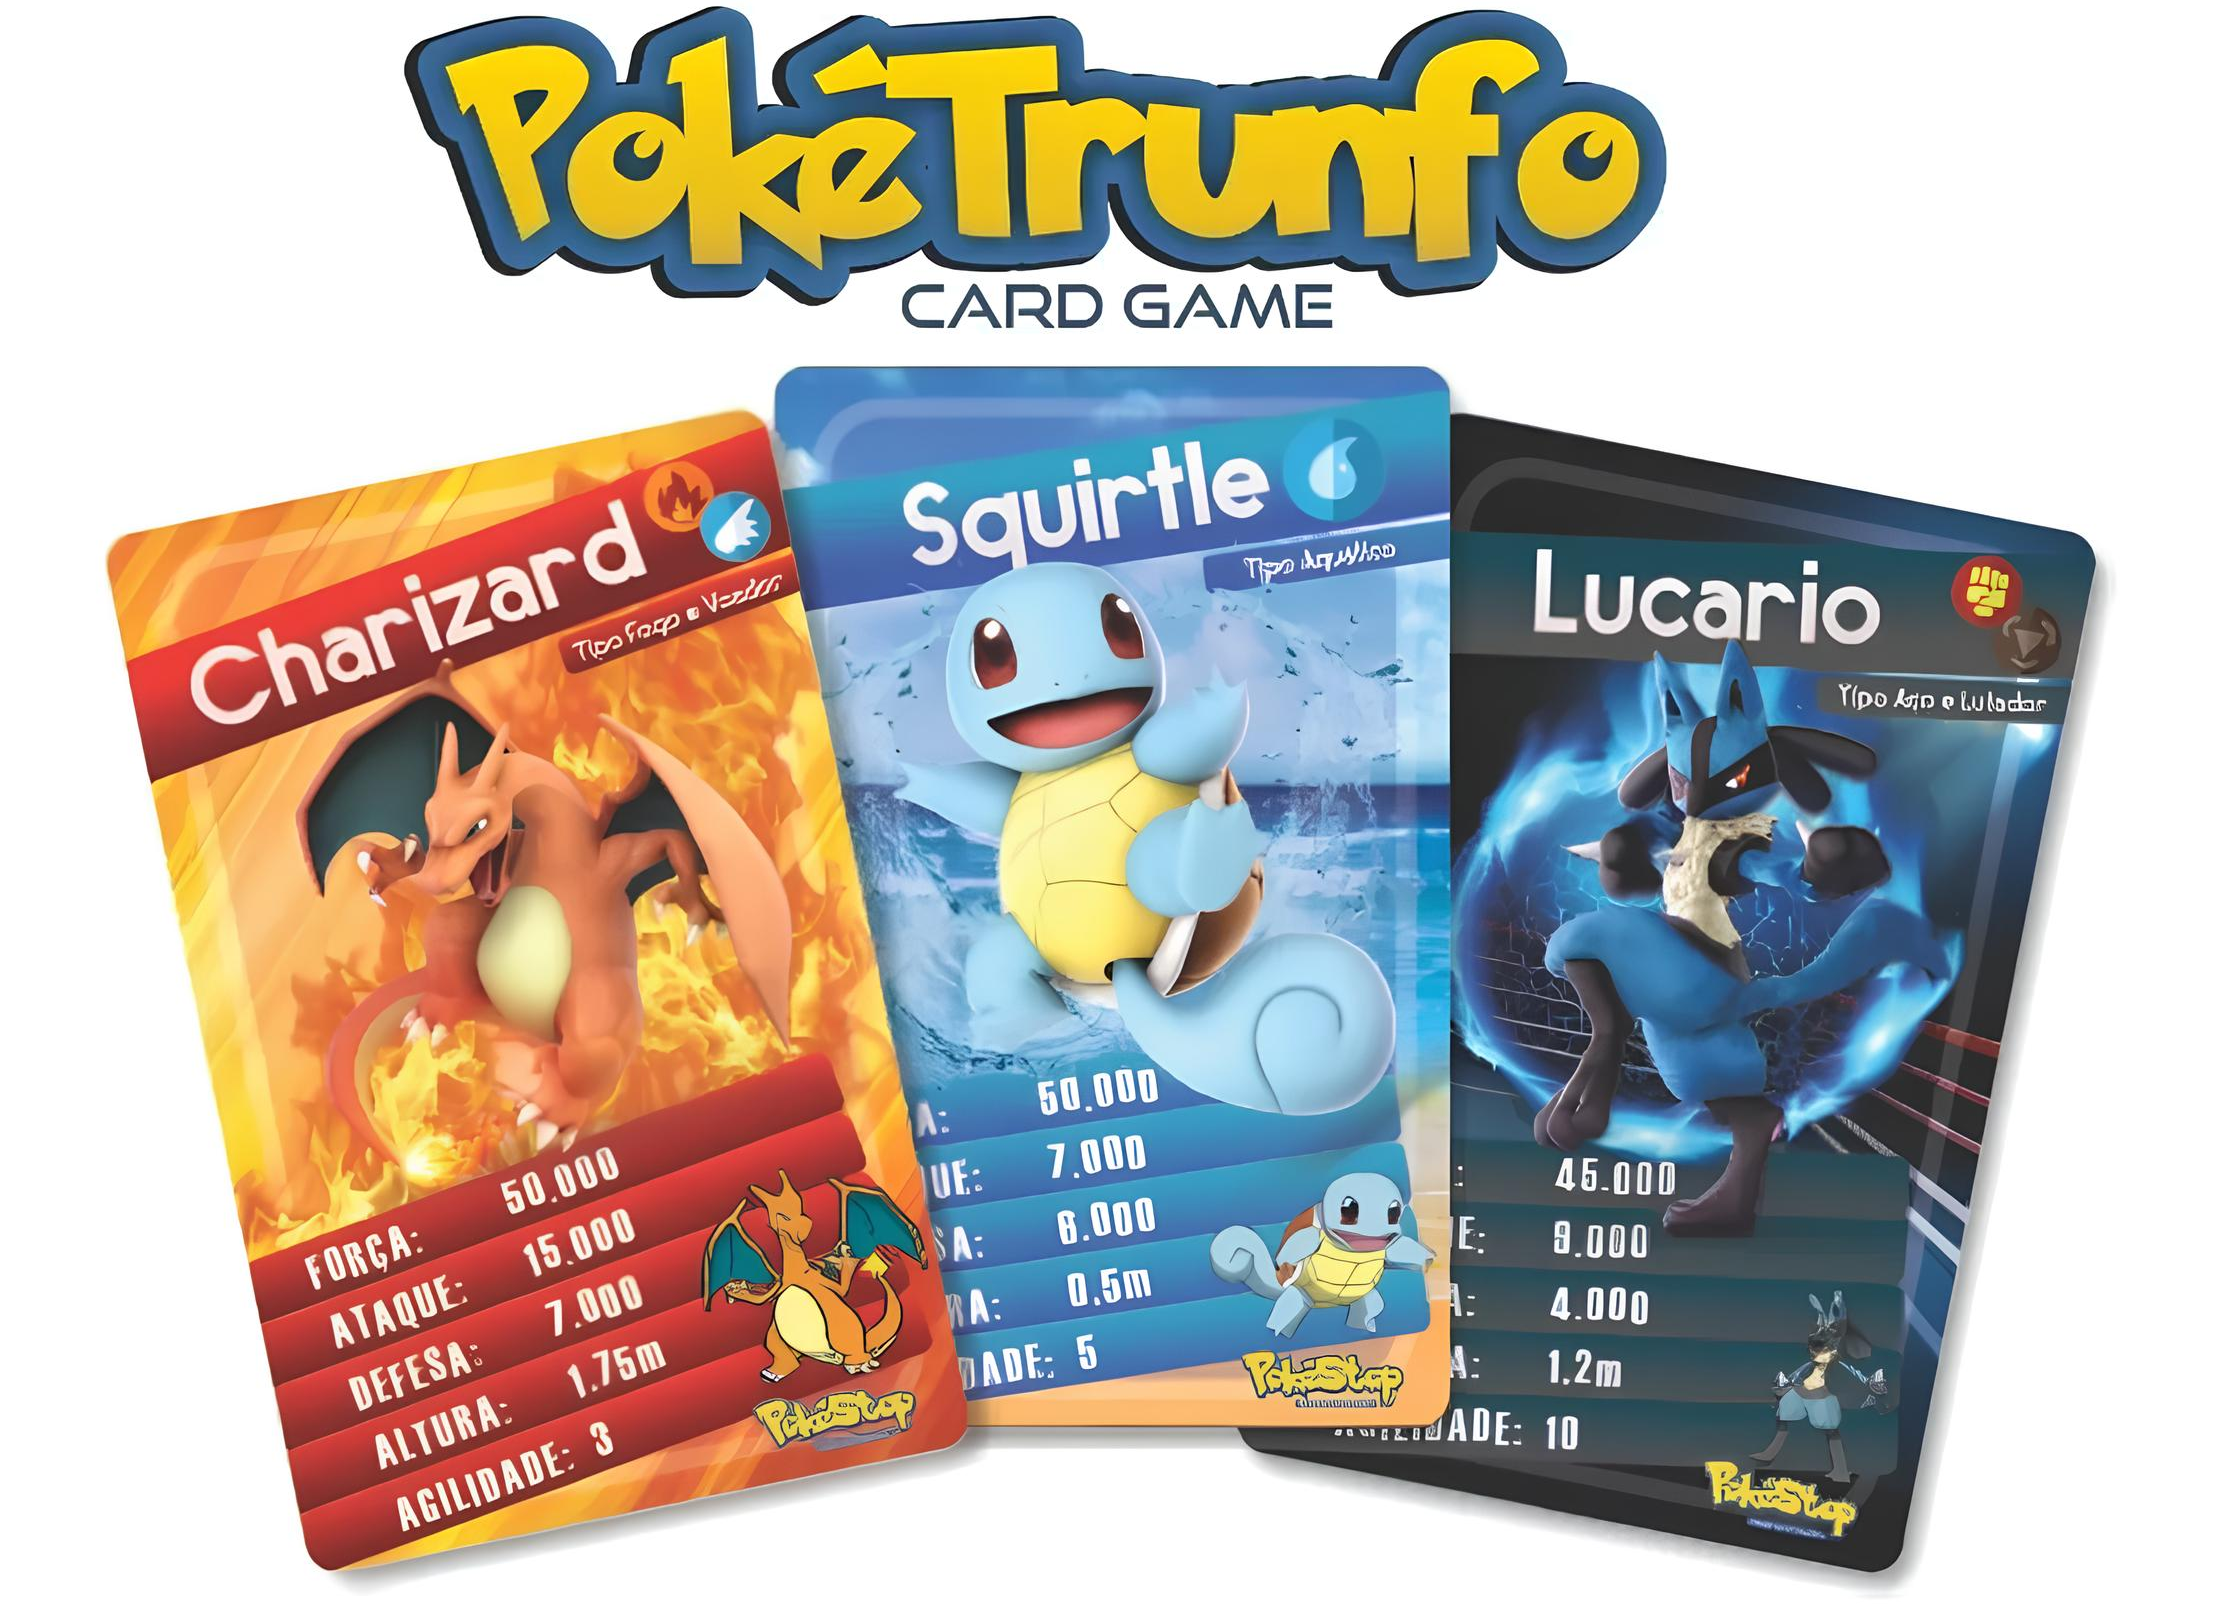
\includegraphics[width=0.7\textwidth]{super-trunfo}
  \legend{Fonte: Loja Grow}
\end{figure}

\subsection{Escolha da dinâmica}
\label{sec:escolha-dinamica}

As três dinâmicas levantadas na fase de refinamento -- Tarot dos Riscos, Amarelinha Game Board e Poke Risk -- foram avaliadas com base em critérios como aplicabilidade, potencial de engajamento dos participantes, duração da dinâmica e viabilidade de implementação. Para validar essa análise inicial e obter uma perspectiva prática sobre a aderência das propostas ao contexto de equipes ágeis, foram realizadas conversas com líderes de projeto do Laboratório Bridge. Suas percepções foram essenciais para a decisão final, conforme detalhado a seguir.

A avaliação conjunta das dinâmicas revelou uma preferência clara pelo \textit{Tarot dos Riscos}, especialmente por sua capacidade de promover maior engajamento e discussões mais aprofundadas sobre os riscos. Em contraste, o \textit{Poke Risk} (Super Trunfo) foi percebido como menos eficaz para o contexto do Laboratório Bridge.

Os principais fatores que fundamentaram a escolha do \textit{Tarot dos Riscos} foram:

\begin{itemize}
    \item \textbf{Engajamento e profundidade da discussão:} A líder de projeto 01 destacou que o \textit{Tarot} "incentiva bastante a discussão das pessoas" e é percebido como mais "divertido". O formato com \textit{post-its} é visto como mais fácil para que todos "participem e se envolvam". Por outro lado, o \textit{Poke Risk} foi descrito como "robótico e sem aprofundamento". 
    \item \textbf{Adaptabilidade ao formato remoto:} Em um ambiente \textit{remote-first} como o do Laboratório Bridge, a viabilidade \textit{online} foi um fator decisivo. O \textit{Tarot} foi avaliado como facilmente adaptável a ferramentas de quadro branco digital, como \textit{FigJam} ou \textit{Miro}, enquanto o \textit{Poke Risk} "não funciona bem no contexto remoto". 
    \item \textbf{Mecanismo de priorização e visão geral:} A mecânica de votação com moedas do \textit{Tarot} foi bem recebida, por ser considerada uma forma que "faz sentido para pensarem e responderem", além de "cortar discussões longas demais pra chegar na prioridade". O líder de projeto 02 ressaltou a vantagem de "ter uma visão ampla de todos os riscos, ver essa mesa completa no final" e "tomar uma decisão vendo o todo, [o que é] mais interessante para análise de riscos de fato". Já o \textit{Poke Risk} poderia gerar priorizações baseadas em sorte ou pessimismo, sem permitir uma visão global. 
    \item \textbf{Reconhecimento e motivação:} A mecânica de moedas no \textit{Tarot} foi associada a um senso de reconhecimento e valorização das contribuições individuais. A líder de projeto 01 observou que "o pessoal gosta muito de ranking, de reconhecimento", e que o \textit{Tarot} recompensa melhor as contribuições para "ganhar", ao passo que no \textit{Poke Risk} "a pessoa vai jogar um número ali chutando e o reconhecimento é menor". 
\end{itemize}

Embora a dinâmica \textit{Amarelinha Game Board} também apresentasse elementos de gamificação, suas características competitivas e a necessidade de cálculos específicos para avaliação de riscos não foram priorizadas nas conversas com os líderes, que concentraram a análise nas duas propostas mais contrastantes.

Com base nessa avaliação e no valioso \textit{feedback} dos líderes do Laboratório Bridge, o \textit{Tarot dos Riscos} foi selecionado como a dinâmica a ser desenvolvida e aplicada. Essa escolha está alinhada ao objetivo de criar uma ferramenta lúdica, engajadora e eficaz para a identificação e análise colaborativa de riscos em projetos ágeis, especialmente em contextos que exigem flexibilidade para formatos presenciais e remotos, como é comum no setor de desenvolvimento de \textit{software}.

Durante as conversas, também foram levantadas sugestões para o aprimoramento do \textit{Tarot dos Riscos}. Foi apontada a importância de que as imagens das cartas estejam mais claramente relacionadas ao conteúdo dos riscos. Além disso, recomendou-se que a dinâmica forneça orientações sobre sua frequência ideal de aplicação — como a cada nova demanda ou em intervalos regulares — garantindo sua relevância contínua ao longo do ciclo de vida do projeto.

\section{Análise e design}
\label{sec:analise-design}

Esta seção descreve o processo de análise e design da dinâmica gamificada, em conformidade com a quarta etapa do \textit{framework} de \citeonline{GARCIA201721}. São apresentados os elementos constitutivos da dinâmica, suas mecânicas de interação, estrutura econômica, regras, estética visual e casos de uso. 

\subsection{Escolha dos componentes do jogo}
\label{sec:escolha-componentes}

A dinâmica é composta por um conjunto de elementos projetados para facilitar a identificação e análise de riscos de forma interativa e engajadora. Os principais componentes são:

\begin{itemize}
  \item \textbf{Cartas de risco:} Elemento central da dinâmica, totalizando 32 cartas. Esse número foi definido com base na taxonomia de riscos de \cite{Taxonomy}, originalmente composta por 64 riscos. A seleção considerou os riscos mais citados tanto no Mapeamento Sistemático da Literatura (MSL) de \citeonline{garcia2023agreed}, quanto na continuidade do mapeamento realizada neste estudo. A soma da frequência de citação em ambos os levantamentos resultou na ordenação e seleção dos 32 riscos mais proeminentes, contemplando 84,4\% dos riscos identificados nos mapeamentos. Os dados detalhados da frequência de citação e a metodologia de seleção dos riscos podem ser consultados na planilha disponível em \href{https://docs.google.com/spreadsheets/d/1eAkx4HNaHIKhkq774zI2VREVNmeKtol5uXiC7Jg-0Sc/edit?usp=sharing}{Google Sheets}.
  \begin{itemize}
    \item \textbf{Aspecto visual:} As cartas possuem ilustrações únicas, geradas com auxílio de inteligência artificial generativa (\href{https://pixlr.com/br/image-generator/}{Pixlr Image Generator}). Os prompts foram adaptados para seguir o estilo “Pokémon”, com personagens que representam os riscos de forma lúdica e amigável. Exemplo de prompt utilizado: “Create a Pokémon-style image of a character related to time control powers. The character must have a friendly expression. The character must explicitly include time-related elements, such as a clock, calendar or timeline. The image must have a solid white background.”.
    
    \item \textbf{Layout e conteúdo:} Cada carta contém:
    \begin{enumerate}
      \item \textbf{Nome lúdico:} Nome criativo vinculado à ilustração (ex: “Cronoguiro” para riscos de cronograma), buscando aumentar o engajamento.
      \item \textbf{Nome técnico do risco:} Termo formal conforme a taxonomia (ex: “Cronograma”).
      \item \textbf{Pergunta principal:} Questão que instiga a reflexão sobre a presença e relevância do risco (ex: “O cronograma é adequado e realista?”).
      \item \textbf{Perguntas auxiliares:} Questões complementares para aprofundar a análise (ex: “Existem dependências externas que podem causar atrasos? O método de estimativa é baseado em dados históricos? Há margem para imprevistos?”).
      \item \textbf{Sinalizador de raridade:} Símbolo visual (losango ou estrela) que indica a “raridade” da carta, inspirado em jogos de cartas colecionáveis.
    \end{enumerate}
    
    \item \textbf{Categorias de risco:} As cartas são seccionadas de acordo com as classes da taxonomia \cite{Taxonomy}, distribuídas entre:
    \begin{itemize}
      \item \textit{Product Engineering}
      \item \textit{Development Environment}
      \item \textit{Product Constraint}
    \end{itemize}
  \end{itemize}

  \item \textbf{Moedas para votação:} A dinâmica utiliza moedas (ou fichas representativas) para a etapa de votação dos riscos, permitindo aos participantes priorizar os riscos que consideram mais críticos para o projeto. 

  \item \textbf{Manual de regras:} Um manual abrangente que provê todas as instruções necessárias para conduzir a dinâmica. Este manual detalha as etapas, as regras, as mecânicas do jogo, e sugestões para gerenciar a discussão e a interação entre os participantes. 

  \item \textbf{\textit{Post-its} e canetas:} Materiais básicos auxiliares que permitem aos participantes escreverem riscos específicos associados a cada carta lida, fomentando a individualização e o detalhamento dos riscos no contexto do projeto. 
\end{itemize}

Os componentes foram concebidos para serem facilmente reproduzíveis tanto em formato físico (impressão das cartas e uso de moedas/fichas simples) quanto adaptáveis para ambientes digitais colaborativos, como plataformas de quadro branco online (e.g., \textit{FigJam}). 

\subsection{Escolha das mecânicas do jogo}
\label{sec:escolha-mecanicas}

As mecânicas do jogo foram projetadas para guiar as interações e o fluxo da dinâmica, desde a apresentação dos riscos até sua priorização colaborativa. O design buscou criar um processo flexível que promovesse o pensamento crítico e a colaboração. Para isso, a dinâmica foi estruturada em duas fases principais. A primeira fase é focada na \textbf{identificação e mapeamento de riscos}, onde os participantes associam os riscos genéricos, apresentados nas cartas, ao contexto real de seus projetos. A segunda fase é a de \textbf{votação e priorização}, que utiliza uma mecânica inspirada na técnica “Buy a Feature” para que a equipe possa, de forma visual e consensual, determinar os riscos mais críticos. Um papel de facilitador também foi definido para guiar o processo, embora a dinâmica permita a auto-organização da equipe. O guia detalhado com o passo a passo para a condução de cada etapa encontra-se no Capítulo \ref{cap:dinamica-execucao}.

\subsection{Estabelecimento da economia do jogo}
\label{sec:economia-jogo}

A economia da dinâmica é um sistema simples e direto, projetado para incentivar a participação ativa dos jogadores e orientar a etapa de priorização dos riscos. Ela se baseia em um único tipo de recurso: as moedas de votação.

\subsubsection{Recursos e ganhos}
O principal e único recurso manipulável pelos jogadores são as moedas. A distribuição das moedas segue um modelo fixo e meritocrático:
\begin{itemize}
\item \textbf{Distribuição inicial fixa:} No início da Etapa 2 (Votação), cada participante recebe uma quantidade fixa de moedas. Esse valor inicial garante que todos os jogadores tenham uma base para participar da priorização, independentemente de sua participação na etapa anterior.
\item \textbf{Ganhos por contribuição:} Para estimular o engajamento e a contribuição na Etapa 1 (Mapeamento dos riscos), moedas adicionais podem ser concedidas de acordo com a quantidade de \textit{post-its} escritos pelo participante. Essa regra busca recompensar a proatividade na identificação de riscos específicos do projeto.
\end{itemize}
Não há outros tipos de recursos a serem ganhos ou perdidos, mantendo a simplicidade da economia focada na priorização. As moedas são um recurso de uso único e são gastas de forma definitiva na Etapa 2 (Votação). Não existem outras formas de gastar moedas além do investimento nos riscos priorizados, e as moedas não retornam ao jogador após a votação.

A economia das moedas exerce impacto significativo na estratégia dos jogadores, influenciando diretamente a dinâmica da priorização:
\begin{itemize}
\item \textbf{Estímulo à participação ativa:} A possibilidade de ganhar moedas adicionais incentiva os participantes a se engajarem na escrita de \textit{post-its} durante a fase de mapeamento. Isso não só aumenta a quantidade de riscos identificados, mas também aprofunda a análise individual e coletiva dos desafios do projeto.
\item \textbf{Poder de voto e priorização forçada:} Com um número limitado de moedas, os jogadores são compelidos a fazer escolhas difíceis e a priorizar os riscos que consideram mais críticos. Isso fomenta discussões mais focadas e um alinhamento sobre as verdadeiras preocupações da equipe.
\item \textbf{Competitividade saudável:} \textit{Feedbacks} dos líderes indicaram que a mecânica de moedas adicionais gera uma leve e saudável competitividade entre os colaboradores para escrever mais \textit{post-its}. Isso, por sua vez, aumenta o engajamento geral e a quantidade de informações geradas.
\end{itemize}

\subsection{Estabelecimento das dinâmicas do jogo (regras)}
\label{sec:dinamicas-regras}

As regras da dinâmica foram estabelecidas para orientar a interação dos participantes com os componentes do jogo, assegurando um fluxo de trabalho colaborativo e produtivo. O design das regras optou por um modelo de avaliação conjunta e facilitada, em vez de turnos individuais estritos, para reforçar a colaboração. Foram definidas diretrizes para gerenciar as discussões, garantindo que o foco permaneça na identificação de riscos e que as divergências de percepção sejam capturadas sem a necessidade de um consenso restrito. O critério de finalização e sucesso da dinâmica foi projetado para não ser uma condição de vitória ou derrota, mas sim a conclusão das etapas de mapeamento e a geração de uma lista priorizada de riscos, valorizando o resultado coletivo.

\subsection{Estabelecer a estética do jogo}
\label{sec:estetica-jogo}

A estética do “Tarot dos Riscos” foi desenvolvida para criar uma experiência que, apesar de tratar de um tema sério como riscos, seja leve, convidativa e engajadora. O sentimento geral transmitido é de diversão e informalidade, buscando desmistificar a gestão de riscos e torná-la mais acessível aos participantes.

\begin{itemize}
\item \textbf{Estilo visual principal:} A inspiração primária no universo Pokémon e a utilização de ilustrações geradas por inteligência artificial conferem às cartas um aspecto amigável e lúdico. Cada imagem é projetada para ser visualmente atraente e, ao mesmo tempo, associar-se de forma criativa ao risco que representa. Não há uma paleta de cores predominante única; as cores variam entre as cartas para diversificar a experiência visual. 
\item \textbf{Narrativa e temática implícita:} A dinâmica não possui uma história ou narrativa subjacente explícita além da inspiração visual das ilustrações. A temática é sugerida pelo nome “Tarot dos Riscos”, que evoca a ideia de “prever o futuro” e antecipar os desafios. Essa analogia com o ato de “ler as cartas” do tarot para obter insights sobre o futuro, combinada com a ação de “colocar as cartas na mesa” durante a dinâmica, reforça a ideia de uma análise proativa e reflexiva dos riscos que podem surgir no projeto. 
\item \textbf{Ambiente de aplicação:} Embora a dinâmica seja projetada para ambientes profissionais e equipes de desenvolvimento de \textit{software}, sua estética sugere um ambiente de aplicação mais descontraído. O objetivo é quebrar a formalidade que muitas vezes cerca o tema da gestão de riscos, promovendo um espaço onde a criatividade e a colaboração fluam mais livremente. 
\item \textbf{Elementos estéticos adicionais:} Além das ilustrações e dos nomes criativos, a raridade das cartas é visualmente representada por ícones de losango ou estrela posicionados abaixo das perguntas nas cartas. Este detalhe visual adiciona um elemento sutil de coleção e diferenciação, enriquecendo a experiência gamificada sem sobrecarregar o design. 
\end{itemize}

\subsection{Elaborar os casos de uso do jogo}
\label{sec:casos-de-uso}

Os casos de uso do Tarot abrangem diversos cenários nos quais a dinâmica pode ser aplicada para maximizar seus benefícios, tanto em contextos de projeto quanto em ambientes de aprendizado. A flexibilidade do jogo permite sua adaptação a diferentes momentos e objetivos, sempre com o foco na identificação e análise de riscos.

\begin{itemize}
\item \textbf{Início de projeto ágil:}
\begin{itemize}
\item \textbf{Momento de aplicação:} Recomendada enfaticamente no \textbf{início de um novo projeto ágil}. 
\item \textbf{Objetivo específico:} O principal objetivo é identificar e priorizar os riscos potenciais que podem impactar o projeto desde suas fases iniciais. Isso permite que a equipe construa um entendimento coletivo dos desafios e possa encaminhá-los para a elaboração de planos de resposta proativos. 
\item \textbf{Resultados esperados:} Uma lista clara e priorizada dos riscos mais relevantes para o projeto, maior alinhamento da equipe sobre os desafios e um aprendizado coletivo sobre o panorama de riscos. 
\end{itemize}
\item \textbf{Aplicações periódicas:}
\begin{itemize}
\item \textbf{Momento de aplicação:} Pode ser utilizada \textbf{periodicamente ao longo do projeto}, em momentos como retrospectivas estendidas ou reuniões de \textit{review} de ciclo de vida. 
\item \textbf{Objetivo específico:} Nesta granularidade, o objetivo é mapear riscos para os próximos períodos de múltiplas \textit{sprints} (não necessariamente para uma única \textit{sprint} devido à granularidade potencial), e acompanhar o \textit{status} dos riscos previamente priorizados. Isso permite uma gestão contínua e adaptativa dos riscos.
\item \textbf{Resultados esperados:} Atualização da lista de riscos priorizados, monitoramento da evolução dos riscos existentes e um ciclo contínuo de aprendizado e adaptação. 
\end{itemize}
\item \textbf{Ambientes educacionais (sala de aula):}
\begin{itemize}
\item \textbf{Momento de aplicação:} A dinâmica pode ser útil em ambientes de sala de aula ou em workshops educacionais. 
\item \textbf{Objetivo específico:} Facilitar o aprendizado sobre gestão de riscos em projetos de \textit{software} para estudantes, proporcionando uma experiência prática e gamificada que torna o conceito de risco mais tangível e a identificação mais intuitiva. 
\item \textbf{Resultados esperados:} Maior compreensão dos diferentes tipos de riscos em projetos de \textit{software}, familiarização com o processo de identificação e análise de riscos, e desenvolvimento de habilidades de pensamento crítico e colaboração em cenários de risco. 
\end{itemize}
\item \textbf{Variações e adaptações:} A flexibilidade da dinâmica é ampliada pela possibilidade de utilizar os \textbf{sub-decks temáticos}. Isso permite que a dinâmica seja aplicada com foco em tipos específicos de riscos (ex: riscos de \textit{Product Engineering}) ou com públicos específicos dentro da equipe (ex: apenas a equipe de desenvolvimento focando em riscos técnicos), tornando a atividade mais relevante e direcionada a necessidades particulares do projeto ou da equipe. 
\end{itemize}

\section{Desenvolvimento da plataforma gamificada}
\label{sec:desenvolvimento-plataforma-gamificada}

A quinta etapa do \textit{framework} preconiza o desenvolvimento da plataforma gamificada, com tarefas que incluem gerenciamento do \textit{sprint}, desenvolvimento da \textit{sprint} (preparação, análise, design, implementação, criação de ativos) e testes (depuração, correção, melhoria e otimização). Este arcabouço é tipicamente direcionado à criação de soluções gamificadas que envolvem um componente de \textit{software} significativo, como aplicativos ou sistemas online.

No contexto deste trabalho, a dinâmica gamificada proposta foi concebida primariamente como uma atividade presencial e baseada em materiais físicos. Portanto, não houve a necessidade de um desenvolvimento de \textit{software} no sentido tradicional de criação de uma plataforma online complexa ou de um sistema interativo com funcionalidades de código. A essência da dinâmica reside na interação facilitada por artefatos tangíveis, como cartas impressas, tabuleiros e outros recursos visuais, que são manuseados pelos participantes em um ambiente colaborativo.

Contudo, para expandir a aplicabilidade da dinâmica e permitir sua utilização em cenários de equipes distribuídas ou remotas, foi realizada uma adaptação para um modelo digital. Essa adaptação consistiu na criação de uma versão dos materiais da dinâmica (cartas, áreas de trabalho) em uma ferramenta de quadro branco online, como o \href{https://www.figma.com/pt-br/figjam/}{\textit{FigJam}}, que pode ser utilizada em conjunto com ferramentas de videoconferência. Essa adaptação não implicou em desenvolvimento de \textit{software} complexo ou na codificação de funcionalidades gamificadas, mas sim na transposição dos elementos físicos para um formato digital manipulável e interativo. A principal tarefa aqui foi a criação de ativos digitais e a organização do espaço virtual para replicação das mecânicas da dinâmica física, em vez de um ciclo completo de desenvolvimento de \textit{software} de uma plataforma dedicada.

Assim, embora a presente pesquisa não tenha envolvido o desenvolvimento de uma “plataforma gamificada” conforme o escopo tradicional do \textit{framework} de \citeonline{GARCIA201721} para soluções baseadas em \textit{software}, a etapa foi cumprida por meio da materialização da dinâmica em seu formato físico e da adaptação para o ambiente digital, visando a flexibilidade de aplicação.

\section{Gerenciamento, monitoramento e medição}
\label{sec:gerenciamento-monitoramento-medicao}

A sexta e última etapa do \textit{framework} de gamificação em engenharia de \textit{software}, proposta por \citeonline{GARCIA201721}, concentra-se no gerenciamento, monitoramento e medição da solução gamificada. Esta fase é crucial para avaliar a eficácia da dinâmica após sua aplicação, identificar pontos de melhoria e verificar o cumprimento dos objetivos estabelecidos na fase inicial do projeto. No escopo deste trabalho, este processo é contemplado integralmente no capítulo \ref{cap:avaliacao}. Abordando:
\begin{itemize}
\item O planejamento da avaliação, incluindo a definição dos critérios, métodos e instrumentos de coleta de dados (como o questionário MEEGA+ adaptado e a coleta de \textit{feedback} qualitativo). 
\item A execução da avaliação, descrevendo os procedimentos e o contexto das aplicações com estudantes e profissionais do mercado. 
\item A análise dos dados coletados, apresentando os resultados quantitativos e qualitativos da percepção dos participantes em relação à dinâmica. 
\item A discussão aprofundada dos resultados, comparando as percepções dos diferentes grupos de aplicação e fornecendo insights sobre os pontos fortes e as áreas de aprimoramento da dinâmica. 
\item A identificação das ameaças à validade que podem influenciar as conclusões deste estudo, garantindo a transparência sobre as limitações da pesquisa. 
\end{itemize}

Dessa forma, esta seção remete ao capítulo \ref{cap:avaliacao} para aprofundamento sobre como a etapa de gerenciamento, monitoramento e medição do \textit{framework} foi operacionalizada e analisada no contexto da avaliação da dinâmica gamificada. 

%------------------------------------------------------------------------------%
%------------------------------------------------------------------------------%

\chapter{Guia de execução da dinâmica}
\label{cap:dinamica-execucao}

Este capítulo tem como objetivo apresentar uma visão geral prática da dinâmica “Tarot dos Riscos”, servindo como um guia conciso para sua preparação e execução. Para compreensão aprofundada da concepção e do design das mecânicas do jogo, recomenda-se consultar o Capítulo \ref{cap:proposta}. Os materiais completos da dinâmica, incluindo o manual de regras detalhado e as cartas, tanto para versão digital quanto para versão física, estão disponíveis para download no \href{https://codigos.ufsc.br/gqs/tarot-dos-riscos}{repositório Códigos UFSC do Grupo GQS}.

\section{Objetivos da dinâmica}
\label{sec:objetivos-dinamica-cap5}

Seus principais objetivos são:

\begin{itemize}
\item \textbf{Facilitar a identificação de riscos:} método interativo e acessível para que equipes detectem riscos potenciais em projetos de \textit{software}.
\item \textbf{Promover a análise colaborativa:} estimular discussão e alinhamento entre membros sobre aplicabilidade, probabilidade e impacto dos riscos.
\item \textbf{Priorizar riscos de forma eficiente:} guiar a equipe na seleção dos riscos mais críticos que exigem atenção imediata e planejamento de respostas.
\item \textbf{Engajar os participantes:} transformar a tarefa de gestão de riscos, que pode ser percebida como árida, em uma atividade lúdica e motivadora.
\item \textbf{Apoiar o aprendizado:} servir como ferramenta pedagógica para equipes e estudantes que buscam compreender melhor os conceitos e a prática da gestão de riscos em um contexto ágil.
\end{itemize}

\section{Materiais da dinâmica}
\label{sec:materiais-dinamica}

A dinâmica pode ser executada tanto em formato presencial quanto online, utilizando materiais adaptados para cada contexto. O foco principal aqui é apresentar os elementos visuais que compõem a dinâmica.

\subsection{Componentes visuais}
\label{sec:componentes-visuais}

Os elementos visuais são cruciais para a experiência gamificada e para a compreensão das informações. Para detalhes completos sobre a concepção de cada componente, consultar a Seção \ref{sec:escolha-componentes} do Capítulo \ref{cap:proposta}.

\begin{itemize}
\item \textbf{Cartas de risco:} As cartas de risco são o elemento central da dinâmica, representando riscos potenciais em projetos de \textit{software}. Cada carta tem estética lúdica inspirada no universo Pokémon e contém informações essenciais para a discussão. A Figura \ref{anatomia-carta} ilustra a estrutura de uma carta, e a Figura \ref{carta-exemplo-tarot} apresenta um exemplo concreto.
\end{itemize}

\begin{figure}[H]
\centering
\caption{\label{anatomia-carta} Anatomia da carta}
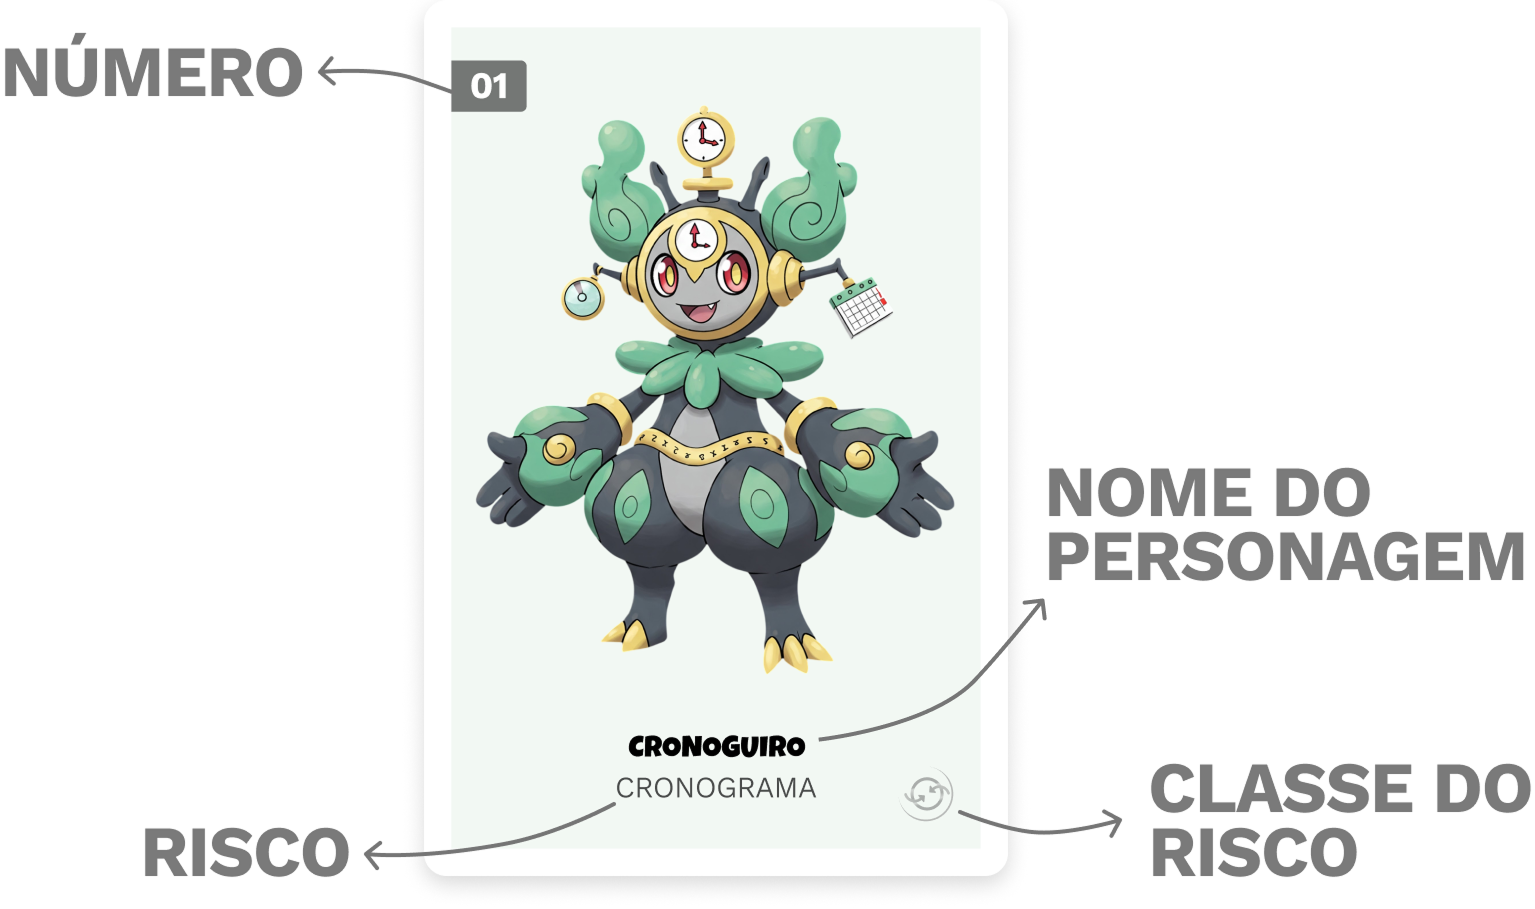
\includegraphics[width=0.5\textwidth]{anatomia-carta}
\legend{Fonte: Autora (2025)}
\end{figure}

\begin{figure}[H]
\centering
\caption{\label{carta-exemplo-tarot} Carta de exemplo (frente e verso)}
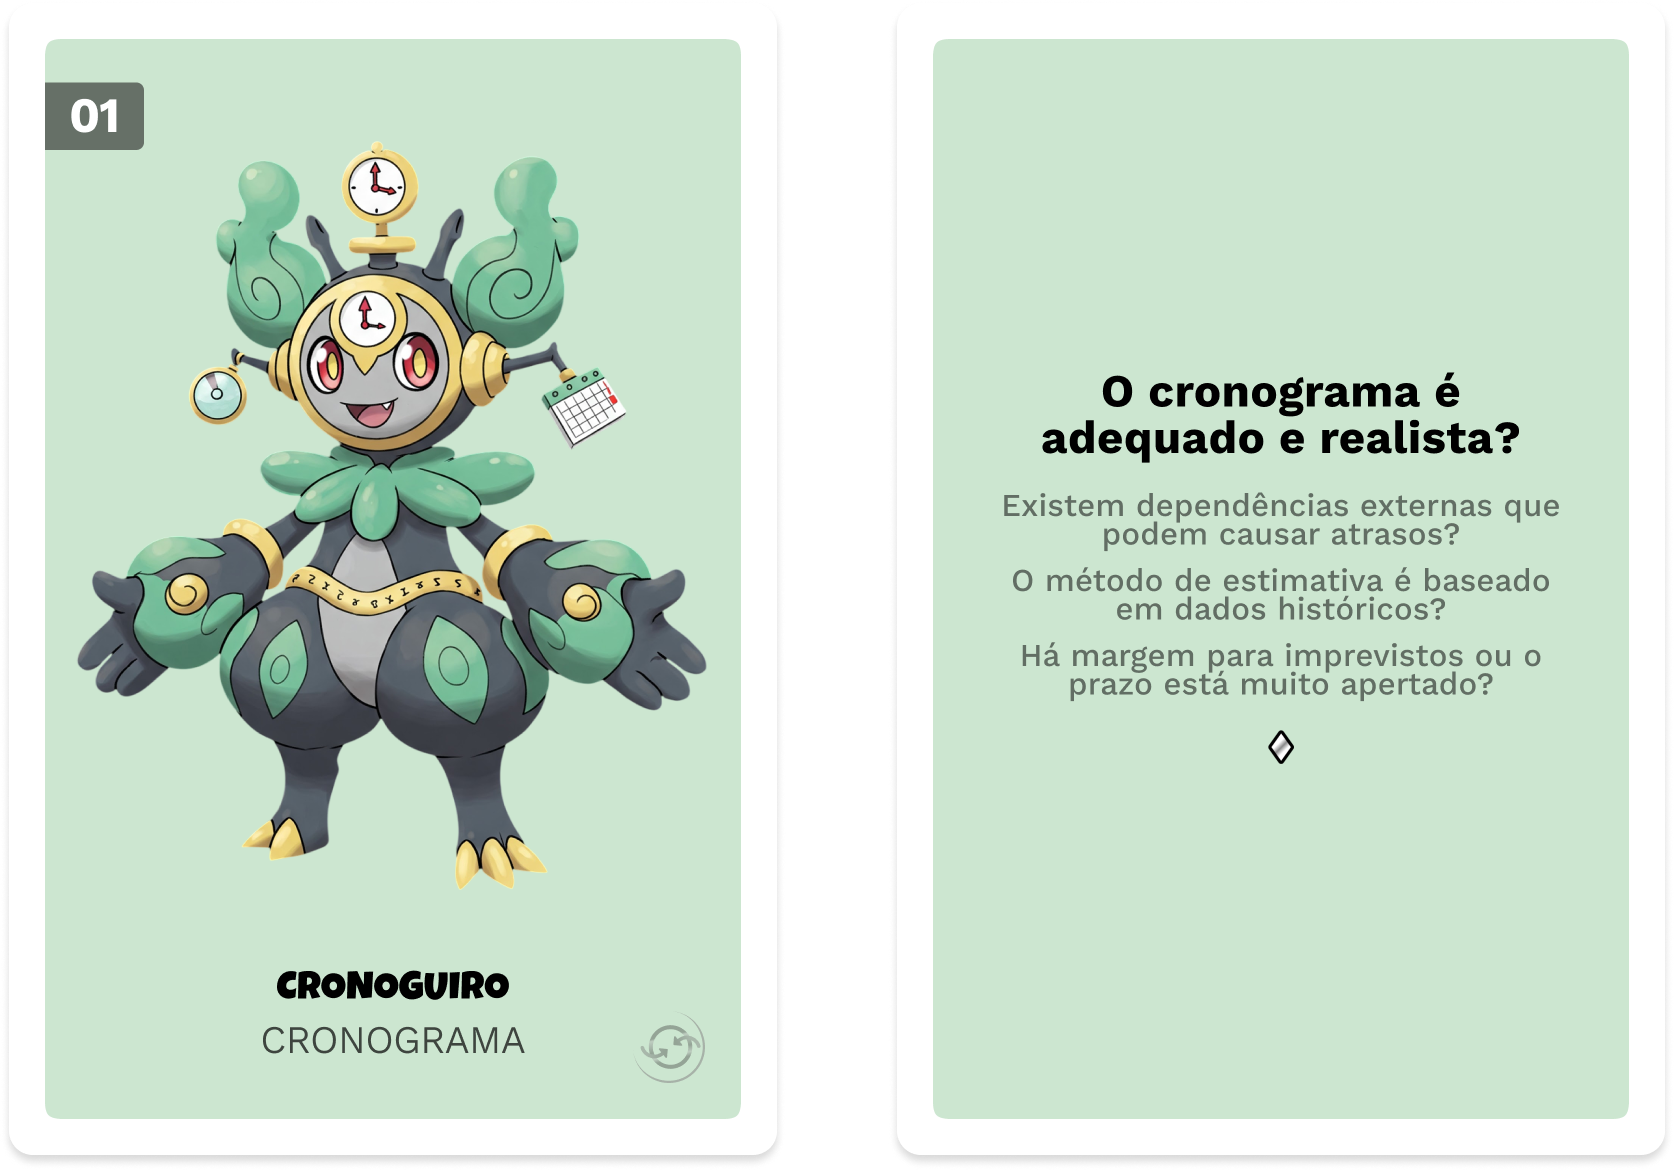
\includegraphics[width=0.7\textwidth]{carta-exemplo-tarot}
\legend{Fonte: Autora (2025)}
\end{figure}

\begin{itemize}
\item \textbf{Manual de regras (Flyer):} Um guia conciso e visual, formatado como um flyer, que condensa as instruções para a execução da dinâmica. Este manual visa facilitar a preparação e dar uma compreensão rápida das regras para os participantes. A Figura \ref{manual-tarot} exibe o formato e o conteúdo principal deste material de apoio.
\end{itemize}

\begin{figure}[H]
\centering
\caption{\label{manual-tarot} Manual de regras (formato \textit{flyer})}
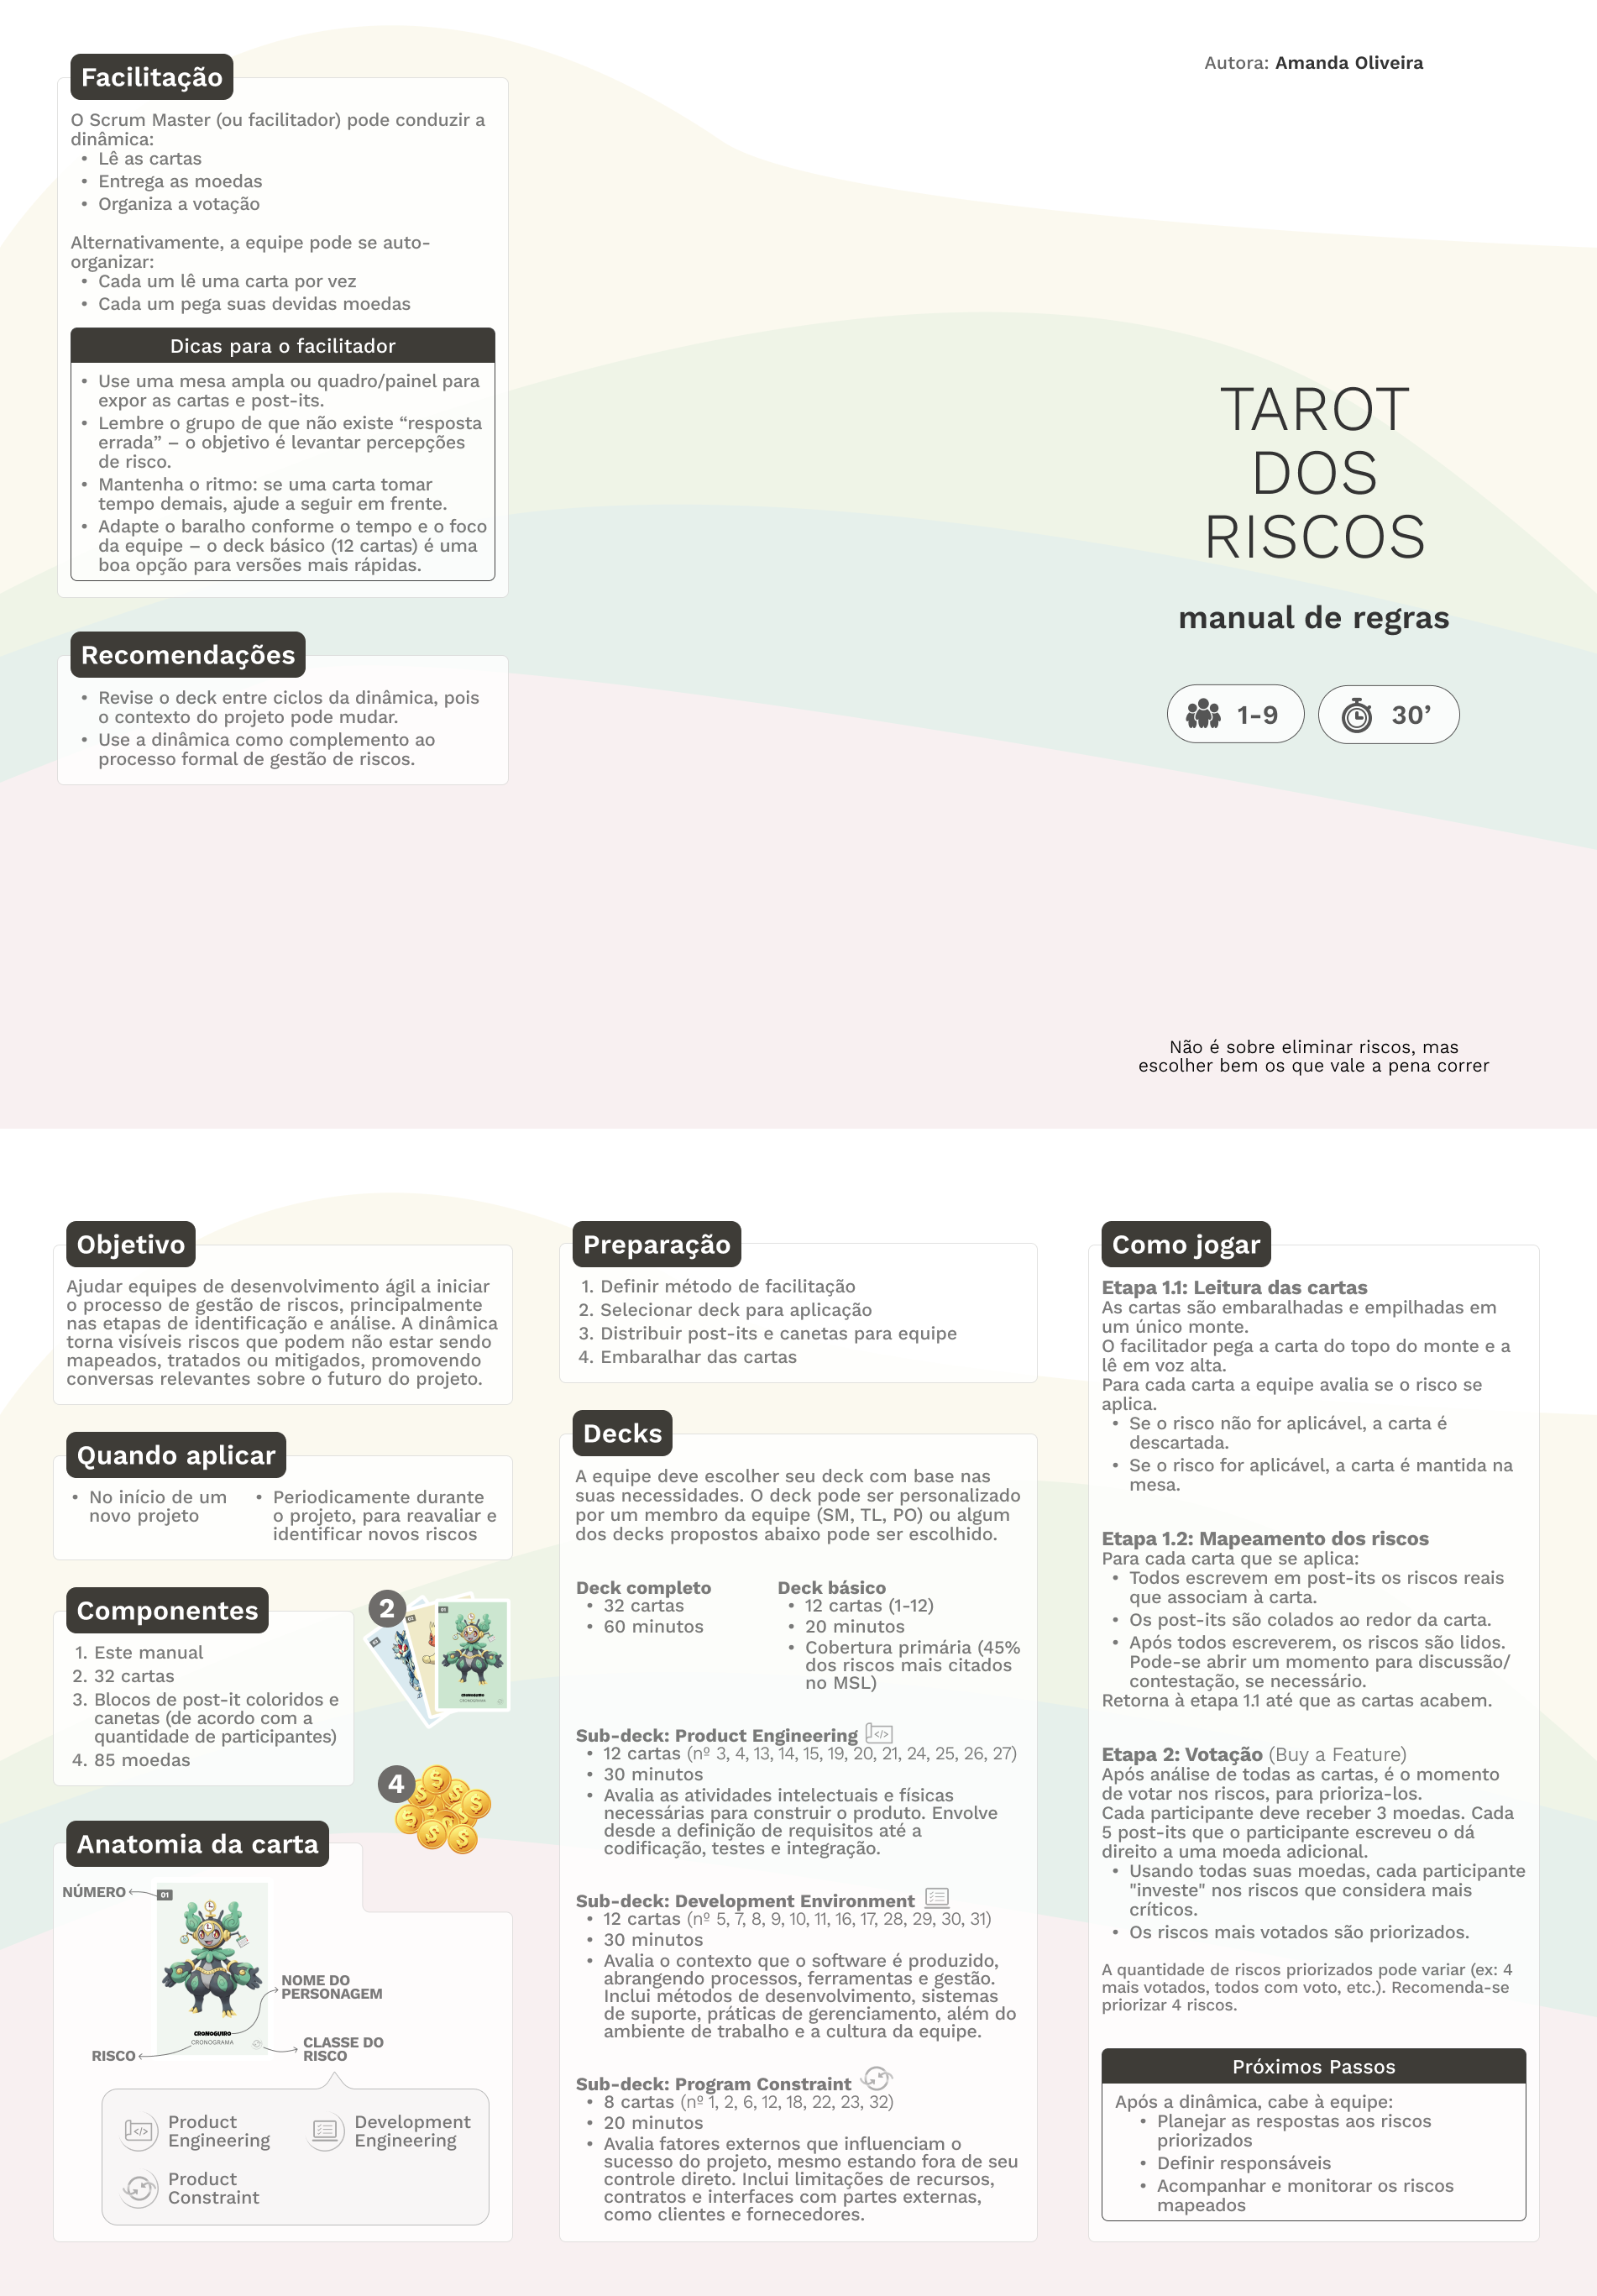
\includegraphics[width=0.85\textwidth]{manual-tarot}
\legend{Fonte: Autora (2025)}
\end{figure}

\begin{itemize}
\item \textbf{Moedas de votação:} Utilizadas na etapa de priorização, as moedas são um componente tátil (em formato físico) ou visual (em formato digital) que permite aos participantes “investir” nos riscos que consideram mais relevantes.
\item \textit{\textbf{Post-its:}} Essenciais para o mapeamento de riscos específicos do projeto, onde os participantes escrevem suas percepções e as associam às cartas de risco.
\end{itemize}

\subsection{Diferenças entre formato presencial e online}
\label{sec:formato-presencial-online}

A dinâmica foi concebida para ser predominantemente presencial, utilizando materiais físicos. No entanto, para ampliar sua aplicabilidade, foi desenvolvida uma adaptação para o ambiente online, sem depender de plataformas de \textit{software} complexas, conforme detalhado na Seção \ref{sec:desenvolvimento-plataforma-gamificada} do Capítulo \ref{cap:proposta}.

\begin{itemize}
\item \textbf{Formato presencial:} Requer a impressão das cartas de risco e das moedas, além da utilização de \textit{post-its}. A dinâmica é conduzida com os participantes reunidos em torno de uma mesa, onde as cartas são dispostas e os \textit{post-its} colados.
\item \textbf{Formato online:} Os materiais (cartas, \textit{post-its}, moedas) são transpostos para uma ferramenta de quadro branco online (ex: \textit{FigJam}, \textit{Miro}). A comunicação e interação entre os participantes são mediadas por ferramentas de videoconferência. A funcionalidade é replicada pela manipulação dos elementos digitais no quadro branco compartilhado. A Figura \ref{dinamica-online} ilustra a dinâmica montada em um ambiente de quadro branco digital.
\end{itemize}

\begin{figure}[H]
\centering
\caption{\label{dinamica-online} Dinâmica em ambiente de quadro branco digital}
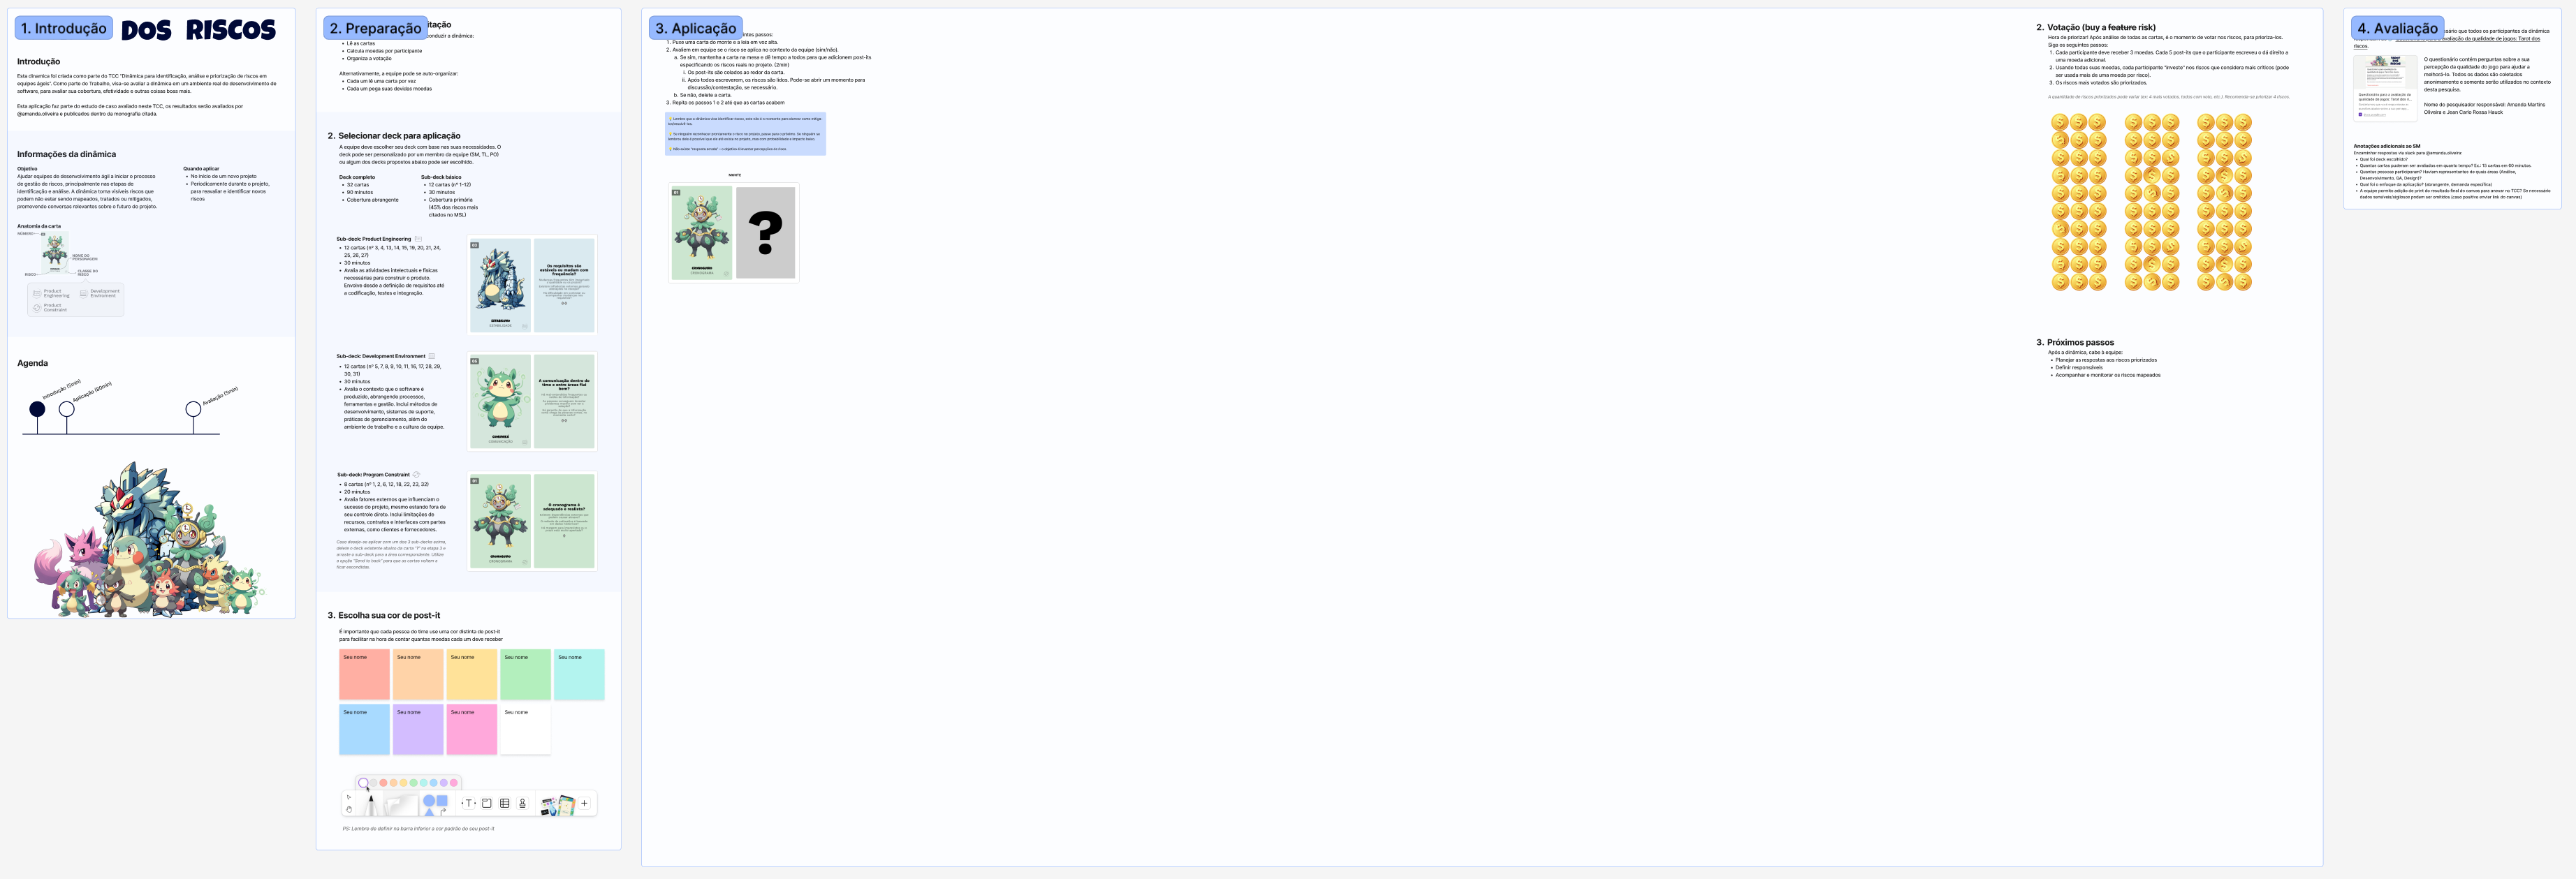
\includegraphics[width=\textwidth]{dinamica-online}
\legend{Fonte: Autora (2025)}
\end{figure}

\section{Preparação para a execução}
\label{sec:preparacao-execucao}

A preparação adequada é fundamental para o sucesso da dinâmica. Antes de iniciar, o facilitador deve:

\begin{enumerate}
    \item \textbf{Escolher o deck de cartas:} Selecionar o deck mais adequado às necessidades da equipe, considerando o tempo disponível e o foco da sessão. A escolha do deck impacta a duração da atividade:
    \begin{itemize}
        \item \textbf{Deck completo (32 cartas):} Ideal para uma análise abrangente. Duração da Etapa 1: aprox. 90 minutos.
        \item \textbf{Deck básico (12 cartas):} Para uma sessão rápida. Duração da Etapa 1: aprox. 30 minutos.
        \item \textbf{Sub-decks temáticos:} Para análises focadas.
        \begin{itemize}
            \item \textit{Product Engineering} (12 cartas): aprox. 30 minutos.
            \item \textit{Development Environment} (12 cartas): aprox. 30 minutos.
            \item \textit{Program Constraint} (8 cartas): aprox. 20 minutos.
        \end{itemize}
    \end{itemize}
    \item \textbf{Organizar os materiais:} Preparar as cartas de risco, as moedas e garantir a disponibilidade de \textit{post-its} e canetas.
    \item \textbf{Familiarizar-se com o manual de regras:} O facilitador deve ler e compreender o manual de regras (conforme Figura \ref{manual-tarot}) para guiar a dinâmica de forma eficaz e intervir quando necessário.
\end{enumerate}

\section{Execução da dinâmica}
\label{sec:execucao-dinamica}

A execução do “Tarot dos Riscos” segue um fluxo lógico e interativo, dividido em duas etapas principais, detalhadas a seguir.

\subsection{Etapa 1: Identificação e mapeamento de riscos}
\label{sec:identificacao-analise-cap5}

Esta etapa inicial foca na associação entre os riscos genéricos (apresentados nas cartas) e os riscos reais e específicos enfrentados pela equipe no seu projeto.

\begin{enumerate}
  \item \textbf{Leitura e avaliação de aplicabilidade:} O facilitador pega uma carta do monte e a lê em voz alta. A equipe avalia coletivamente se o risco é aplicável ao projeto. Se qualquer membro identificar o risco como uma preocupação real, a carta é mantida na mesa. Caso contrário, é descartada.
  \item \textbf{Mapeamento dos riscos reais:} Para cada carta aplicável, os participantes escrevem individualmente em \textit{post-its} os riscos práticos e específicos do projeto que se relacionam com a carta lida. Os \textit{post-its} são então agrupados ao redor da carta correspondente. Após a escrita, o facilitador lê os riscos registrados e abre um momento para discussão e alinhamento, mantendo o foco na análise e evitando desviar para a busca de soluções.
  \begin{figure}[H]
      \centering
      \caption{\label{mapeamento-riscos-postits} Mapeamento de riscos com \textit{post-its} (exemplo de aplicação)}
      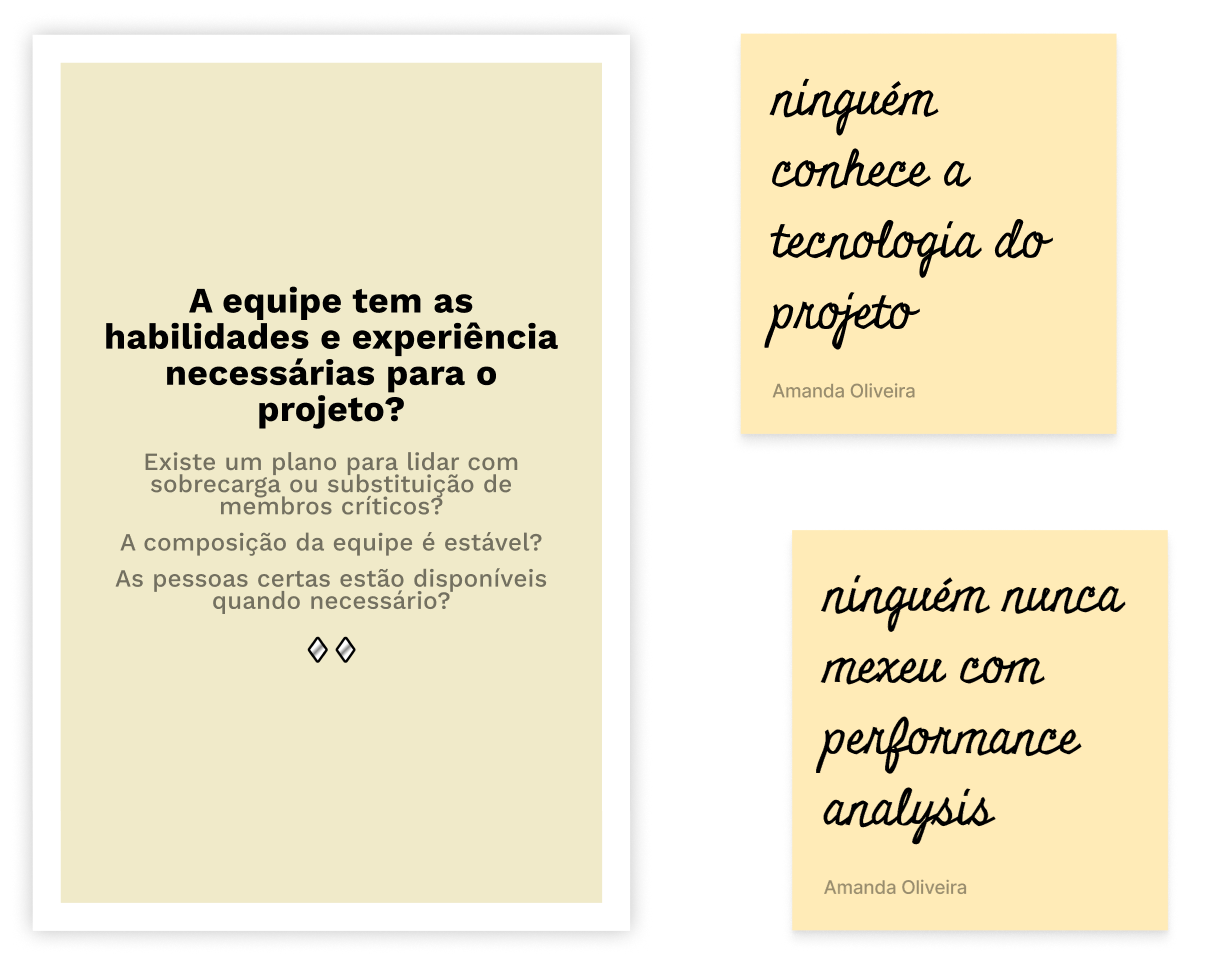
\includegraphics[width=0.6\textwidth]{mapeamento-riscos-postits}
      \legend{Fonte: Autora (2025)}
  \end{figure}
\end{enumerate}
Este processo de leitura e mapeamento é repetido até que todas as cartas do deck escolhido sejam avaliadas.

\subsection{Etapa 2: Votação e priorização de riscos}
\label{sec:priorizacao-riscos-cap5}

Após o mapeamento, a equipe avança para a priorização, que utiliza uma mecânica inspirada na técnica “\textit{Buy a Feature}”. Esta etapa é mais rápida e objetiva, com uma duração recomendada de 5 minutos.

\begin{enumerate}
  \item \textbf{Distribuição de moedas:} Cada participante recebe uma quantidade inicial fixa de 3 moedas. Para incentivar a contribuição na etapa anterior, os jogadores recebem 1 moeda adicional a cada 5 \textit{post-its} que escreveram. Essa regra visa recompensar a proatividade e o engajamento na identificação de riscos.
  \item \textbf{Investimento nos riscos:} Com as moedas em mãos, cada participante as distribui entre os \textit{post-its} ou as cartas de risco que considera mais críticos para o projeto. As moedas representam o "investimento" para tratar aquele risco, e o número limitado força uma priorização cuidadosa.
  \begin{figure}[H]
      \centering
      \caption{\label{votacao-moedas} Priorização de riscos com moedas de votação (exemplo de aplicação)}
      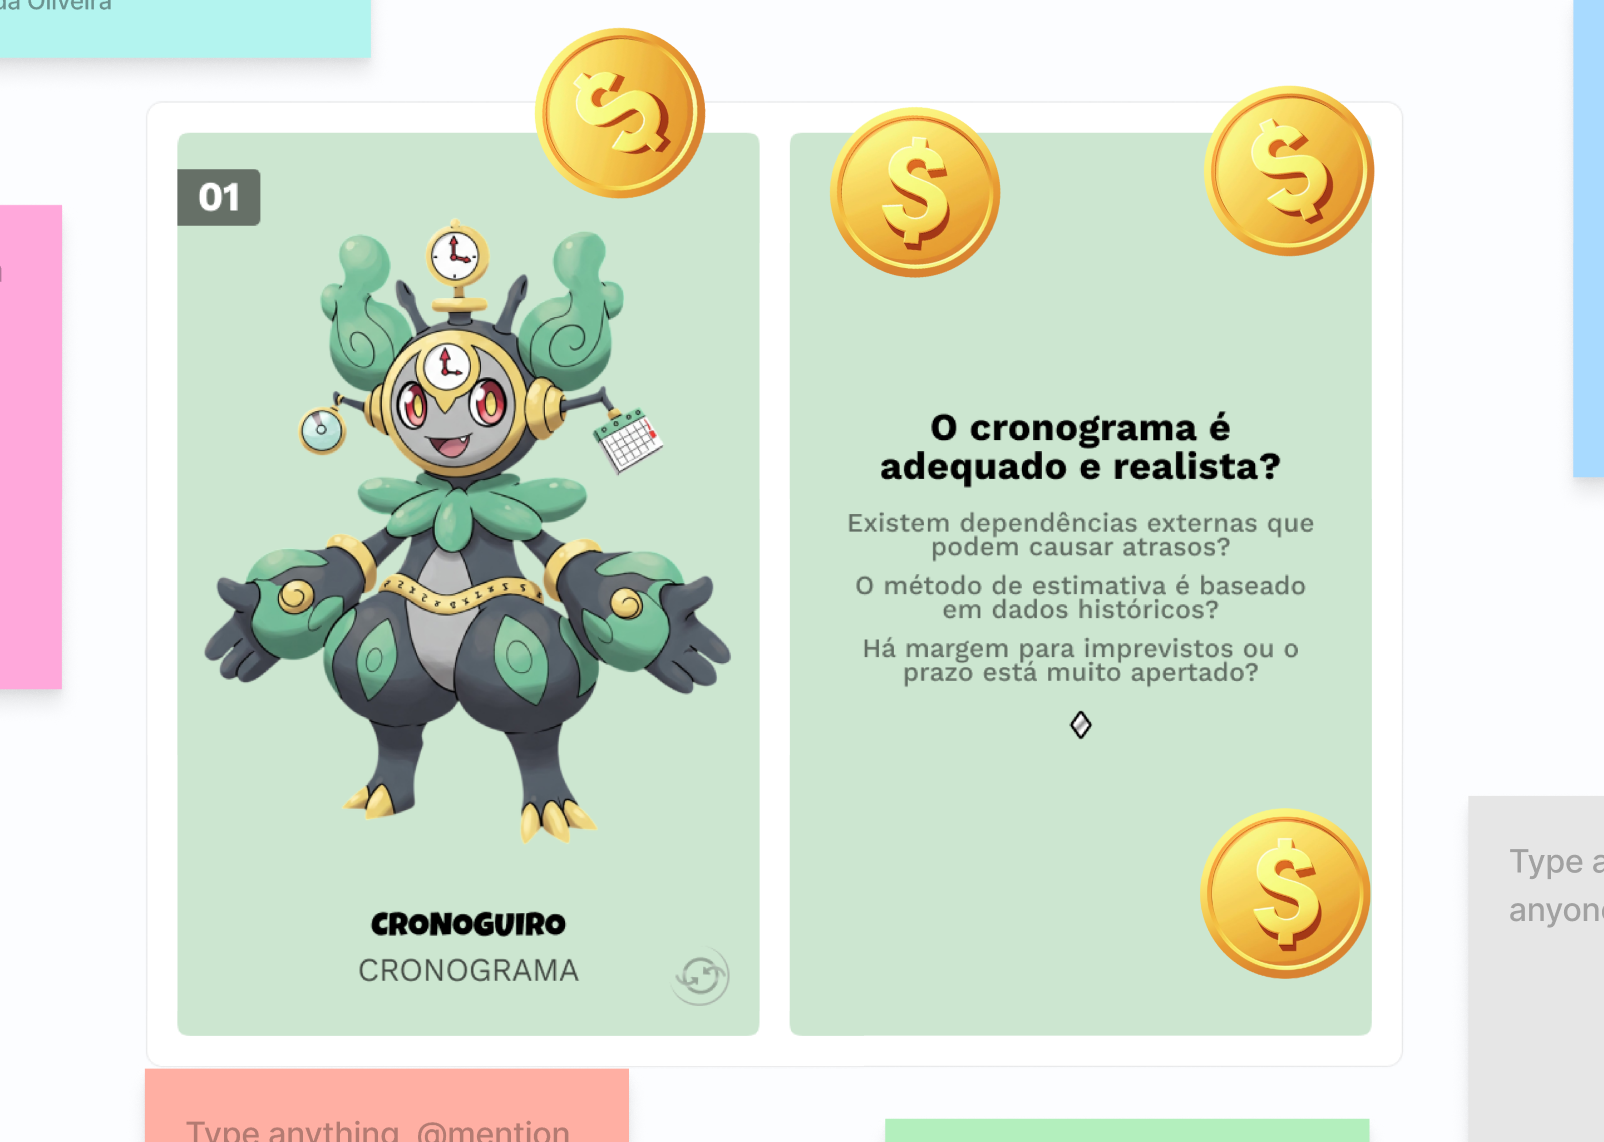
\includegraphics[width=0.6\textwidth]{votacao-moedas}
      \legend{Fonte: Autora (2025)}
  \end{figure}

  \item \textbf{Priorização:} Após a votação, os riscos são classificados com base na quantidade de moedas que acumularam. Quanto mais moedas, maior a prioridade. Recomenda-se que a equipe selecione os 4 riscos mais votados para focar no planejamento de respostas. Em caso de empate, a equipe pode realizar uma discussão rápida ou uma votação de desempate.
\end{enumerate}

\subsection{O papel do facilitador}

O facilitador (\textit{Scrum Master}, \textit{Tech Lead}, ou outro membro com essa habilidade) é fundamental para garantir a condução eficaz da dinâmica. Suas responsabilidades incluem:

\begin{itemize}
  \item \textbf{Preparação}: Escolha e organização do deck de cartas e de todos os materiais necessários.
  \item \textbf{Condução das etapas}: Leitura das cartas, gerenciamento do fluxo das discussões e coordenação da distribuição e contagem das moedas.
  \item \textbf{Mediação}: Garantir que a discussão permaneça focada na identificação e análise de riscos, intervindo quando necessário para evitar desvios para soluções ou mitigações.
  \item \textbf{Gestão do tempo}: Embora flexível, o facilitador deve monitorar o tempo para que todas as etapas sejam concluídas de forma produtiva.
\end{itemize}

Alternativamente, a equipe pode optar pela auto-organização, onde os próprios membros se revezam nas funções do facilitador, promovendo ainda mais a autonomia e a colaboração.

\section{Considerações finais}
\label{sec:consideracoes-finais-cap5}

A dinâmica “Tarot dos Riscos” oferece uma abordagem inovadora e prática para a gestão de riscos em equipes ágeis, promovendo a proatividade e a colaboração. Seu formato gamificado e a flexibilidade de adaptação para ambientes presenciais e online a tornam uma ferramenta valiosa para equipes que buscam otimizar seus processos de identificação e análise de riscos. Ao final da dinâmica, as equipes terão uma visão clara dos principais desafios e um ponto de partida sólido para o planejamento de ações mitigadoras, contribuindo para projetos mais resilientes e bem-sucedidos. Os resultados da aplicação da dinâmica e sua avaliação são detalhados no Capítulo \ref{cap:avaliacao}.

Por se tratar de uma dinâmica que pode conter evoluções futuras, caso o usuário tenha sugestões ao criador deste trabalho, é possível que seja feito contato por e-mail: \texttt{amanda.martins.oliveira@grad.ufsc.br} para discutir tal evolução. %A explicação de como a dinâmica pode ser implementada está disponibilizada por vídeo em: <>.

De antemão, a autora agradece a utilização da dinâmica e espera que seja útil em seus projetos de \textit{software}.

% TODO: Adicionar gravação de vídeo explicando a dinâmica

%------------------------------------------------------------------------------%
%------------------------------------------------------------------------------%

\chapter{Avaliação}
\label{cap:avaliacao}

Neste capítulo, é apresentada a avaliação da dinâmica proposta. A avaliação é um passo crucial para verificar a eficácia, aplicabilidade e usabilidade da dinâmica em diferentes contextos e com diferentes perfis de participantes.

Será detalhado o planejamento da avaliação, incluindo a metodologia empregada e as adaptações realizadas no método MEEGA+. Em seguida, descreve-se a execução da avaliação, dividida em duas abordagens distintas: uma com a participação de estudantes e outra com profissionais da área de desenvolvimento de \textit{software}. Para cada uma dessas avaliações, serão apresentados os métodos de coleta e análise dos dados. Por fim, o capítulo traz uma discussão dos resultados obtidos, comparando as percepções dos grupos, e finaliza com a discussão das ameaças à validade que podem influenciar as conclusões do estudo.

\section{Planejamento da avaliação}

Para garantir a validade e a robustez dos resultados da dinâmica proposta, foi utilizado o modelo MEEGA+ (\textit{Method for an Extensive and Exhaustive Game Assessment}) de \citeonline{MEEGA}, um \textit{framework} consolidado para a avaliação da qualidade de jogos.

A escolha do MEEGA+ justifica-se por sua capacidade de fornecer um instrumento de medição confiável e estruturado. Sua abordagem abrangente se alinha aos objetivos desta pesquisa, permitindo avaliar a dinâmica para identificação de riscos. O modelo desdobra fatores de qualidade em métricas relacionadas à motivação, experiência do usuário e aprendizado. Essa granularidade é fundamental para compreender o impacto da dinâmica e identificar pontos de melhoria, indo além de uma simples avaliação de engajamento, e adentrando em aspectos como a eficácia na facilitação do aprendizado e na análise de riscos.

A próxima subseção detalha como o MEEGA+ foi adaptado para o contexto específico desta dinâmica, bem como os procedimentos adotados para a coleta de dados.

\subsection{Adaptação do MEEGA+}

Ao empregar o modelo MEEGA+ para a avaliação da dinâmica gamificada proposta neste trabalho, foram necessárias algumas adaptações específicas. O MEEGA+ foi concebido para a avaliação de jogos educacionais, porém o Tarot não se configura como um jogo tradicional, mas sim como uma atividade gamificada, que aplica elementos e mecânicas de jogos no contexto de análise de riscos.

Durante o processo de planejamento desta avaliação, foi realizada uma análise para identificar os elementos do modelo MEEGA+ original que não se mostravam aplicáveis ou alinhados aos objetivos específicos da dinâmica. Assim, a customização envolveu a remoção de certas afirmativas do questionário padrão que não refletiam a natureza ou o propósito da gamificação do Tarot. Vale ressaltar que, embora essas adaptações permitam uma avaliação mais direcionada e focada, a modificação de um instrumento validado pode, em certa medida, afetar a comparabilidade direta com resultados obtidos com o modelo original e sua validade/confiabilidade no novo contexto.

Com base nessa análise, foram removidas as seguintes afirmativas do questionário MEEGA+, conforme as justificativas apresentadas na Tabela~\ref{tab:afirmativas-removidas}:

\begin{table}[h!]
  \centering
  \caption{Afirmativas do MEEGA+ removidas e suas justificativas.}
  \label{tab:afirmativas-removidas}
  \begin{tabular}{|p{0.35\textwidth}|p{0.65\textwidth}|}
  \hline
  \textbf{Afirmativa removida} & \textbf{Justificativa de exclusão} \\ \hline
  O jogo oferece novos desafios em um ritmo adequado & A dinâmica não possui ritmo intrínseco de desafios que se assemelhe a um jogo tradicional. Seu foco é na facilitação da discussão e análise. \\ \hline
  É devido ao meu esforço pessoal que eu consigo avançar no jogo & A dinâmica de análise de riscos é uma atividade colaborativa, onde o avanço é construído em equipe, e não depende primariamente do esforço individual. \\ \hline
  Eu estava tão envolvido no jogo que eu perdi a noção do tempo & Embora o engajamento seja desejável, esta afirmativa remete a uma imersão típica de jogos de entretenimento ou com narrativa intensa, que não é o foco principal de uma ferramenta para análise de riscos. \\ \hline
  Eu esqueci sobre o ambiente ao meu redor enquanto jogava este jogo & Similar à afirmativa anterior, esta métrica foca em um nível de imersão que não é o objetivo central de uma dinâmica profissional de análise de riscos. \\ \hline
  \end{tabular}
  \legend{Fonte: Autora (2025)}
\end{table}

De forma complementar, foram adicionadas perguntas customizadas, conforme a flexibilidade sugerida pelo próprio MEEGA+ para abordar objetivos específicos. Essas novas afirmativas foram elaboradas para avaliar a eficácia da dinâmica na promoção da identificação e análise de riscos, um dos principais objetivos deste trabalho, e estão detalhadas na Tabela~\ref{tab:afirmativas-adicionadas}.

\begin{table}[H]
  \centering
  \caption{Afirmativas customizadas adicionadas e suas justificativas.}
  \label{tab:afirmativas-adicionadas}
  \begin{tabular}{|p{0.45\textwidth}|p{0.55\textwidth}|}
  \hline
  \textbf{Afirmativa adicionada} & \textbf{Justificativa de inclusão} \\ \hline
  A dinâmica contribuiu para reconhecer os principais riscos que podem afetar o andamento do projeto. & Essencial para verificar se a dinâmica cumpriu seu objetivo principal de auxiliar na identificação de riscos relevantes. \\ \hline
  A dinâmica contribuiu para reconhecer de forma clara e consciente os riscos presentes no projeto. & Avalia a clareza e a profundidade da percepção dos riscos após a utilização da ferramenta. \\ \hline
  A dinâmica contribuiu para aumentar a percepção da equipe sobre suas vulnerabilidades diante de falhas ou imprevistos. & Visa medir o impacto da dinâmica na conscientização coletiva sobre a fragilidade do projeto e a necessidade de mitigação. \\ \hline
  A dinâmica contribuiu para exercitar a análise inicial dos riscos levantados em equipe. & Verifica se a ferramenta não apenas identifica, mas também fomenta a discussão e análise colaborativa dos riscos, aspecto-chave em métodos ágeis. \\ \hline
  \end{tabular}
  \legend{Fonte: Autora (2025)}
\end{table}

\section{Execução da avaliação}

A avaliação da dinâmica proposta foi conduzida em duas etapas distintas, visando coletar \textit{feedback} de diferentes perfis de participantes: estudantes e profissionais. Esta seção detalha a execução de cada uma dessas avaliações.

\subsection{Avaliação com estudantes}

Como etapa inicial da avaliação da dinâmica de gamificação para identificação e análise de riscos, foram realizadas aplicações em sala de aula com estudantes de graduação. As sessões ocorreram em maio de 2025, envolvendo alunos das disciplinas INE5427 (Planejamento e Gestão de Projetos) e INE5617 (Gerência de Projetos) do Departamento de Informática e Estatística (INE) da Universidade Federal de Santa Catarina (UFSC).

Participaram um total de 45 estudantes, todos regularmente matriculados nos cursos de Ciência da Computação ou Sistemas de Informação da UFSC. Após a aplicação da dinâmica, 30 desses participantes responderam ao questionário de avaliação baseado no modelo MEEGA+ adaptado.

As aplicações foram divididas em dois turnos (matutino e noturno), seguindo um protocolo semelhante em ambos:

\begin{itemize}
  \item \textbf{Momento inicial:} Iniciava-se com uma explanação sobre o trabalho, os objetivos da dinâmica e suas regras gerais.
  \item \textbf{Execução da dinâmica:} Os alunos eram separados em grupos para a realização das etapas da dinâmica.
  \item \textbf{Questionário:} Ao final, os participantes eram convidados a responder ao questionário de avaliação.
\end{itemize}

Detalhes específicos de cada turma:

\begin{itemize}
  \item \textbf{Primeira turma (matutino):} Contou com 18 alunos, divididos em grupos de 4 ou 5 integrantes. Para a primeira etapa da dinâmica (leitura e mapeamento dos riscos), foram concedidos 30 minutos. Para a segunda etapa (votação/priorização dos riscos), foram alocados 5 minutos adicionais. Os grupos receberam os materiais necessários da dinâmica (cartas, manual, \textit{post-its} e canetas) e uma folha contendo uma descrição fictícia de um projeto de \textit{software} (disponível no \hyperref[apendiceD]{Apêndice D}) para contextualizar a aplicação.
  \item \textbf{Segunda turma (noturno):} Contou com 27 alunos, divididos em grupos de 5 ou 6 integrantes. O tempo alocado para a primeira etapa foi de 20 minutos, e para a segunda etapa, 5 minutos. O processo de aplicação e distribuição de materiais foi similar ao da primeira turma.
\end{itemize}

\begin{figure}[H]
  \centering
	\caption{\label{aplicacao-aula-alunos} Aplicação da dinâmica com estudantes}
  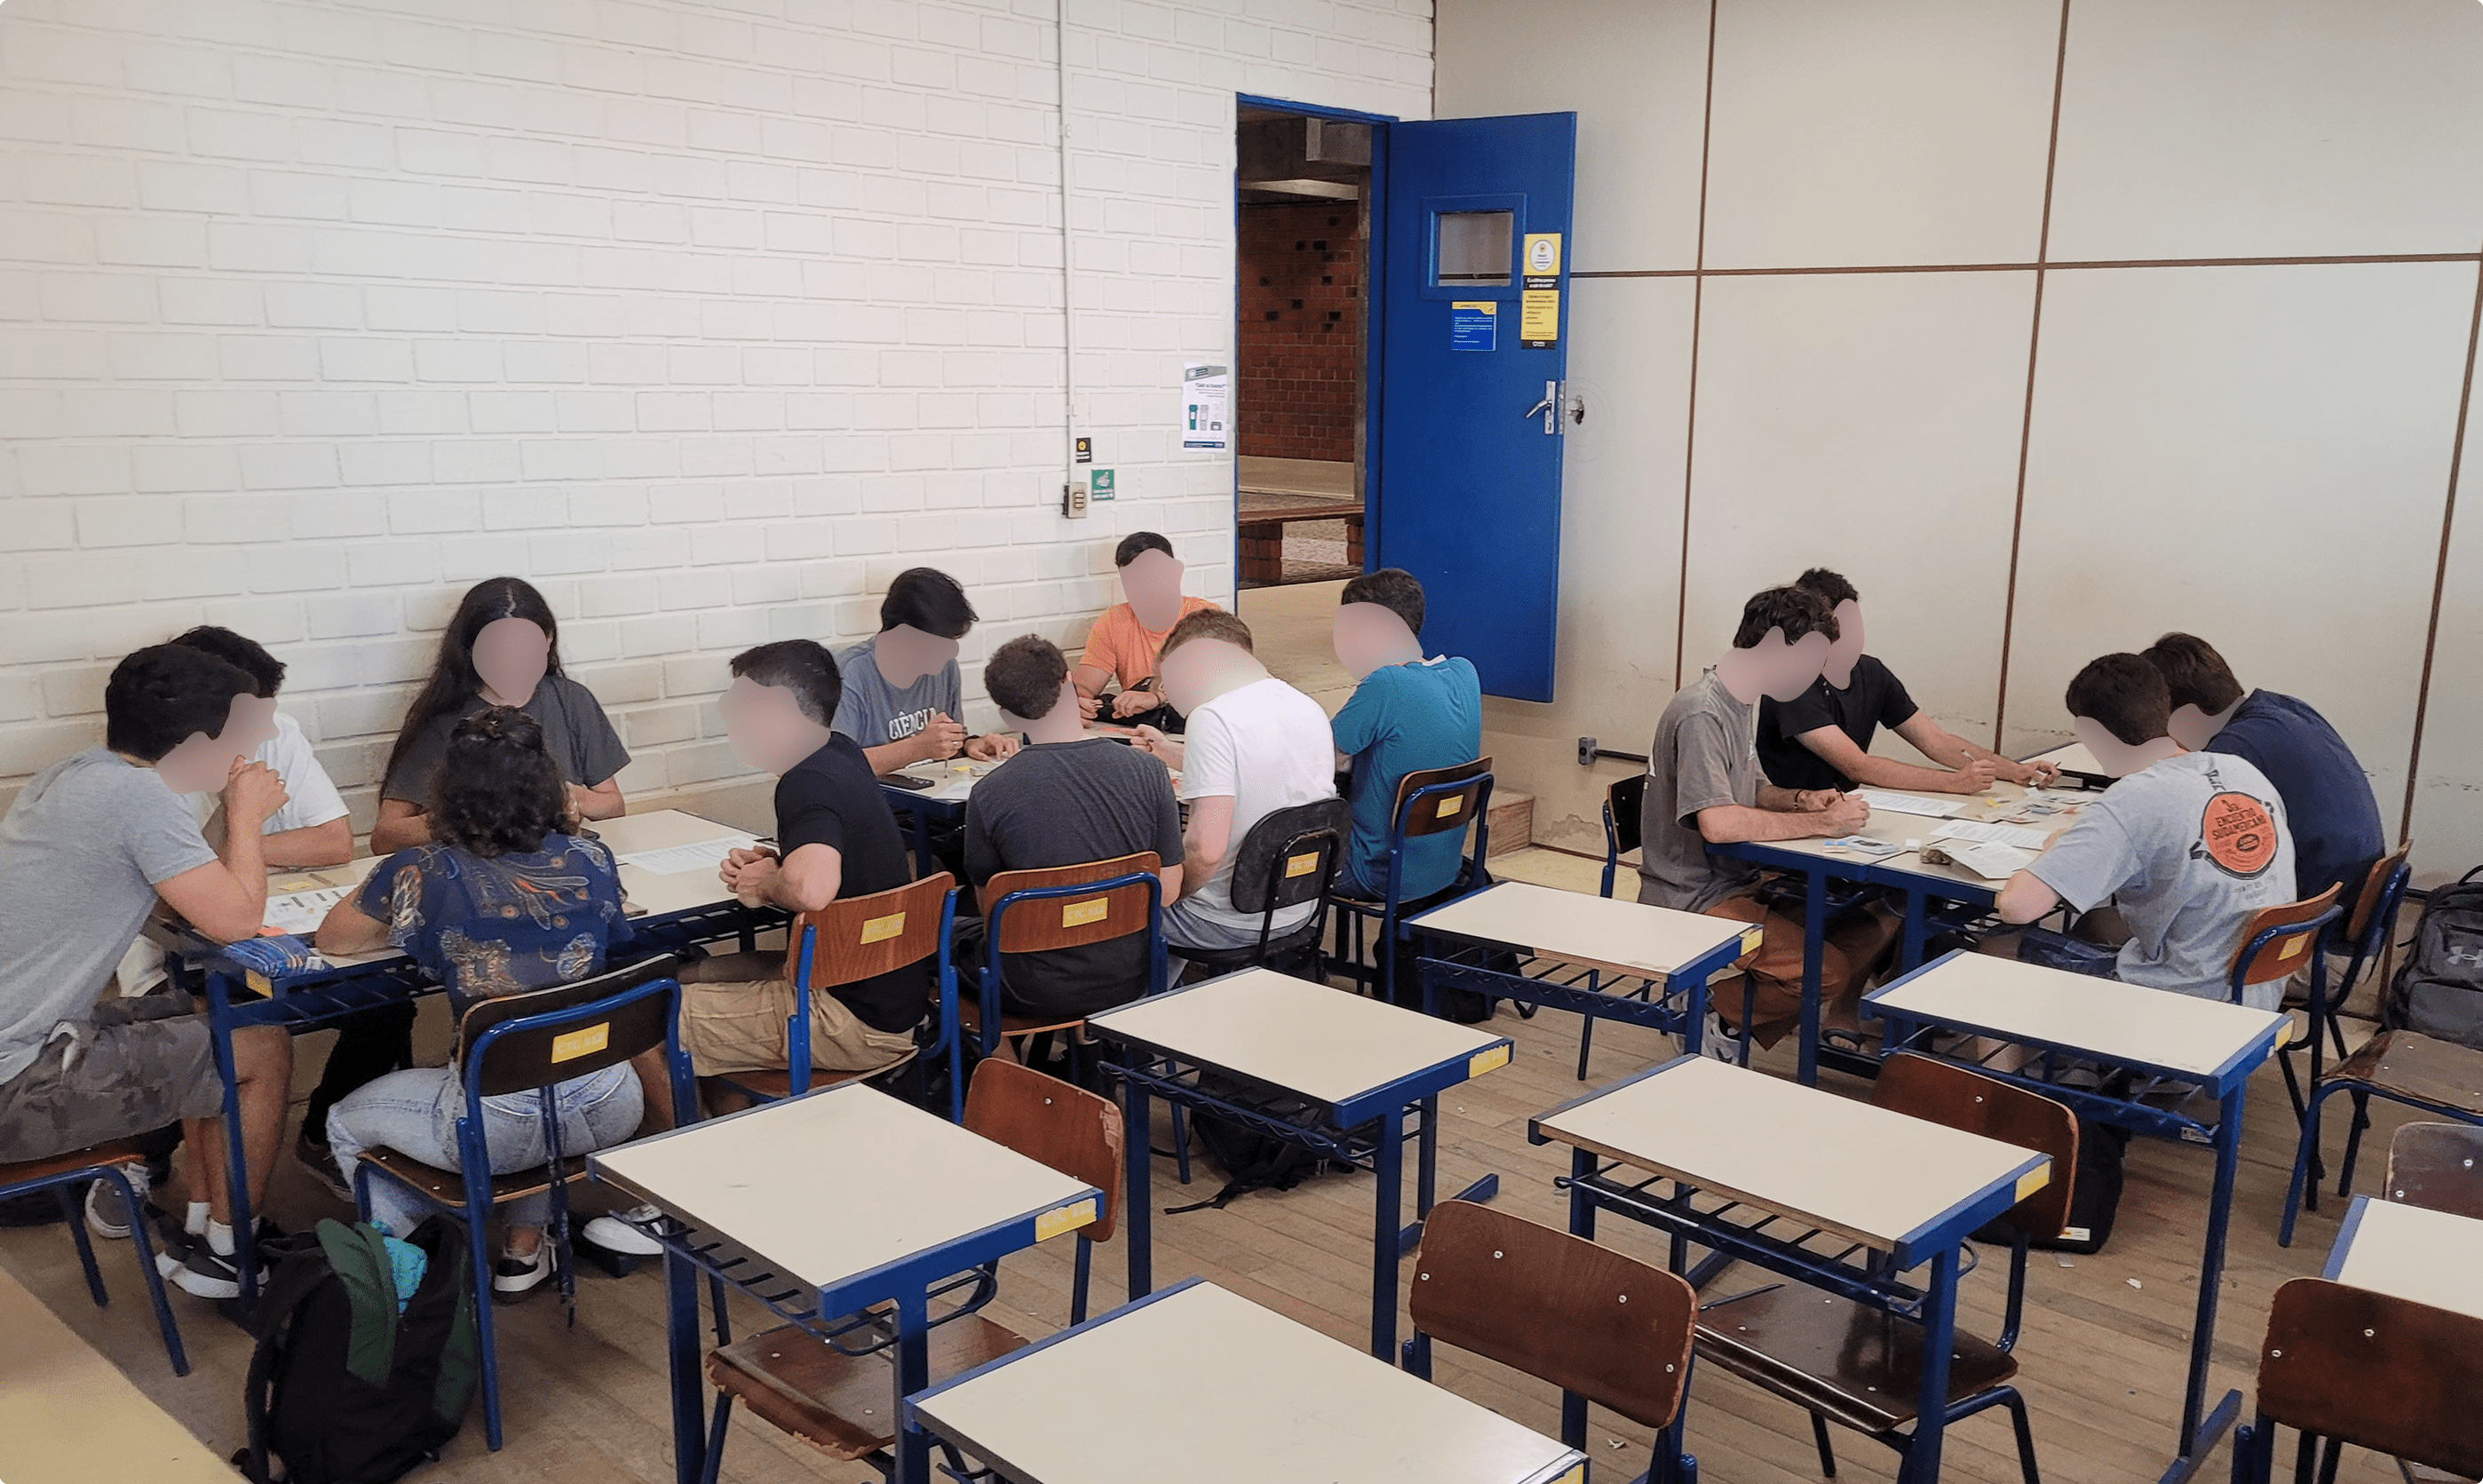
\includegraphics[width=\textwidth]{aplicacao-aula-alunos}
	\legend{Fonte: Autora (2025)}
\end{figure}

É importante ressaltar que no formulário de avaliação foi obtida a autorização dos participantes para a coleta de imagens anonimizadas durante a atividade, com o propósito exclusivo de registro e análise da pesquisa acadêmica.

\begin{figure}[H]
  \centering
	\caption{\label{aplicacao-aula-mesa-1} Organização das cartas pelos estudantes 01}
  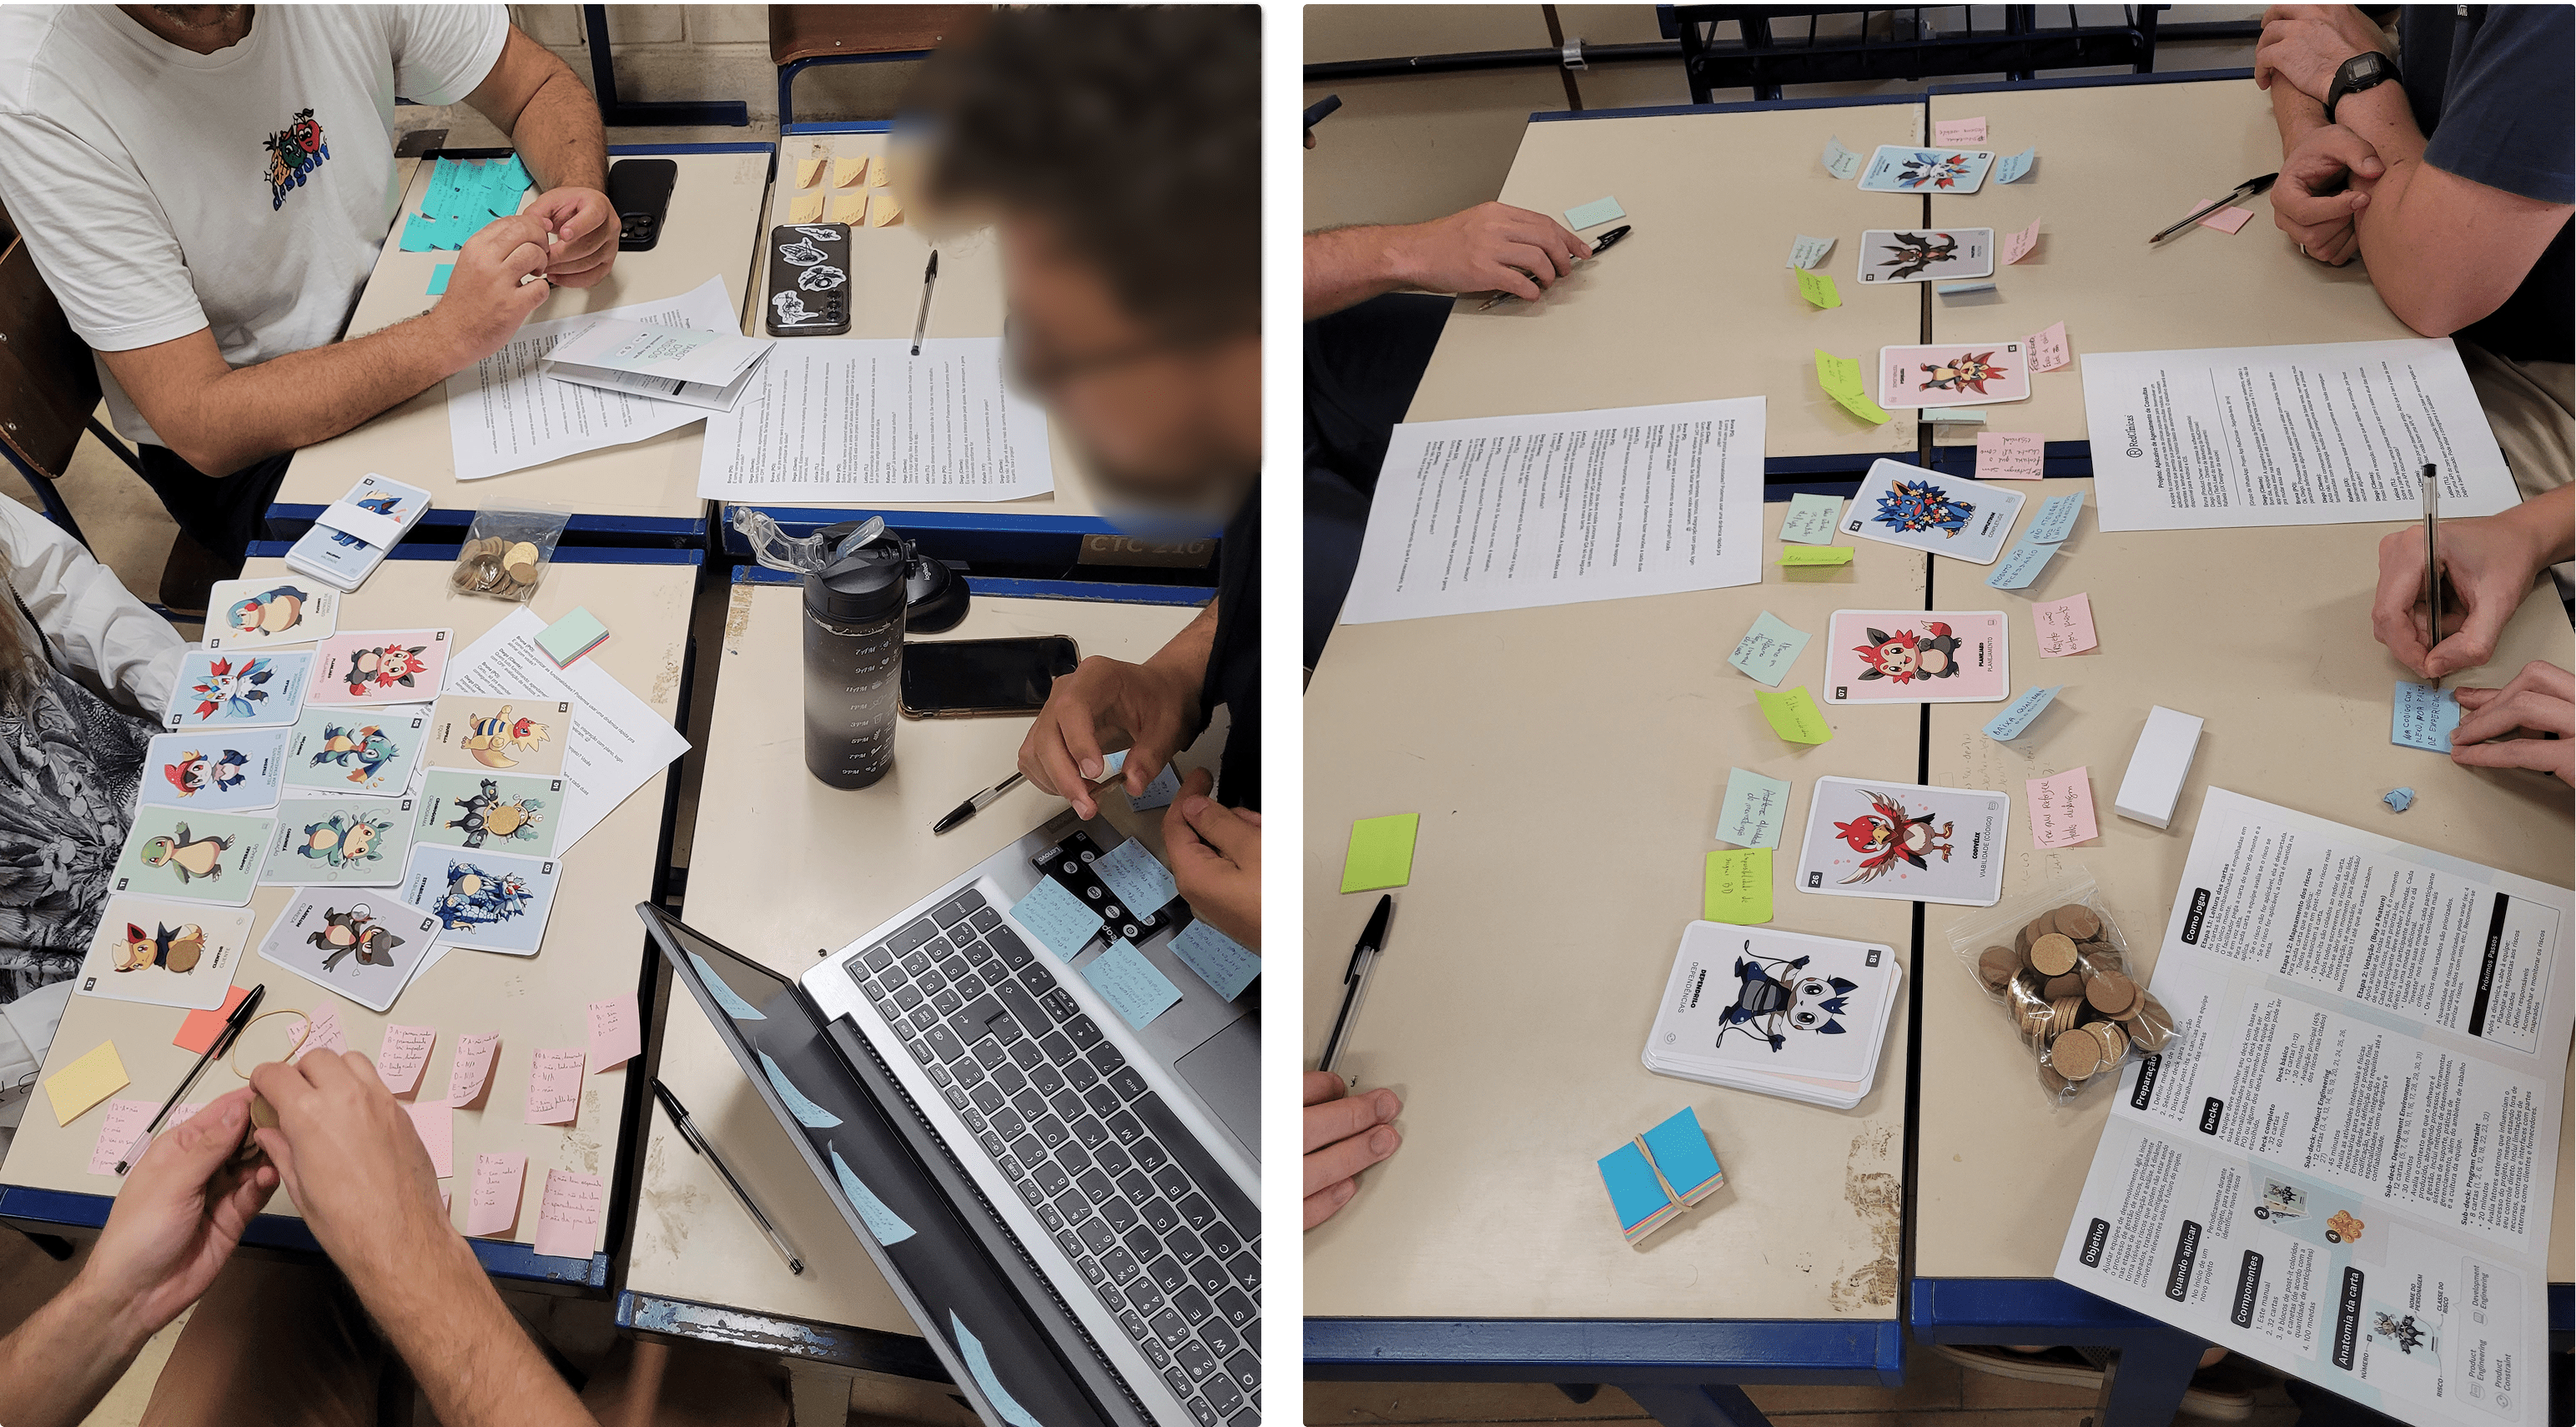
\includegraphics[width=0.8\textwidth]{aplicacao-aula-mesa-1}
	\legend{Fonte: Autora (2025)}
\end{figure}

\begin{figure}[H]
  \centering
	\caption{\label{aplicacao-aula-mesa-2} Organização das cartas pelos estudantes 02}
  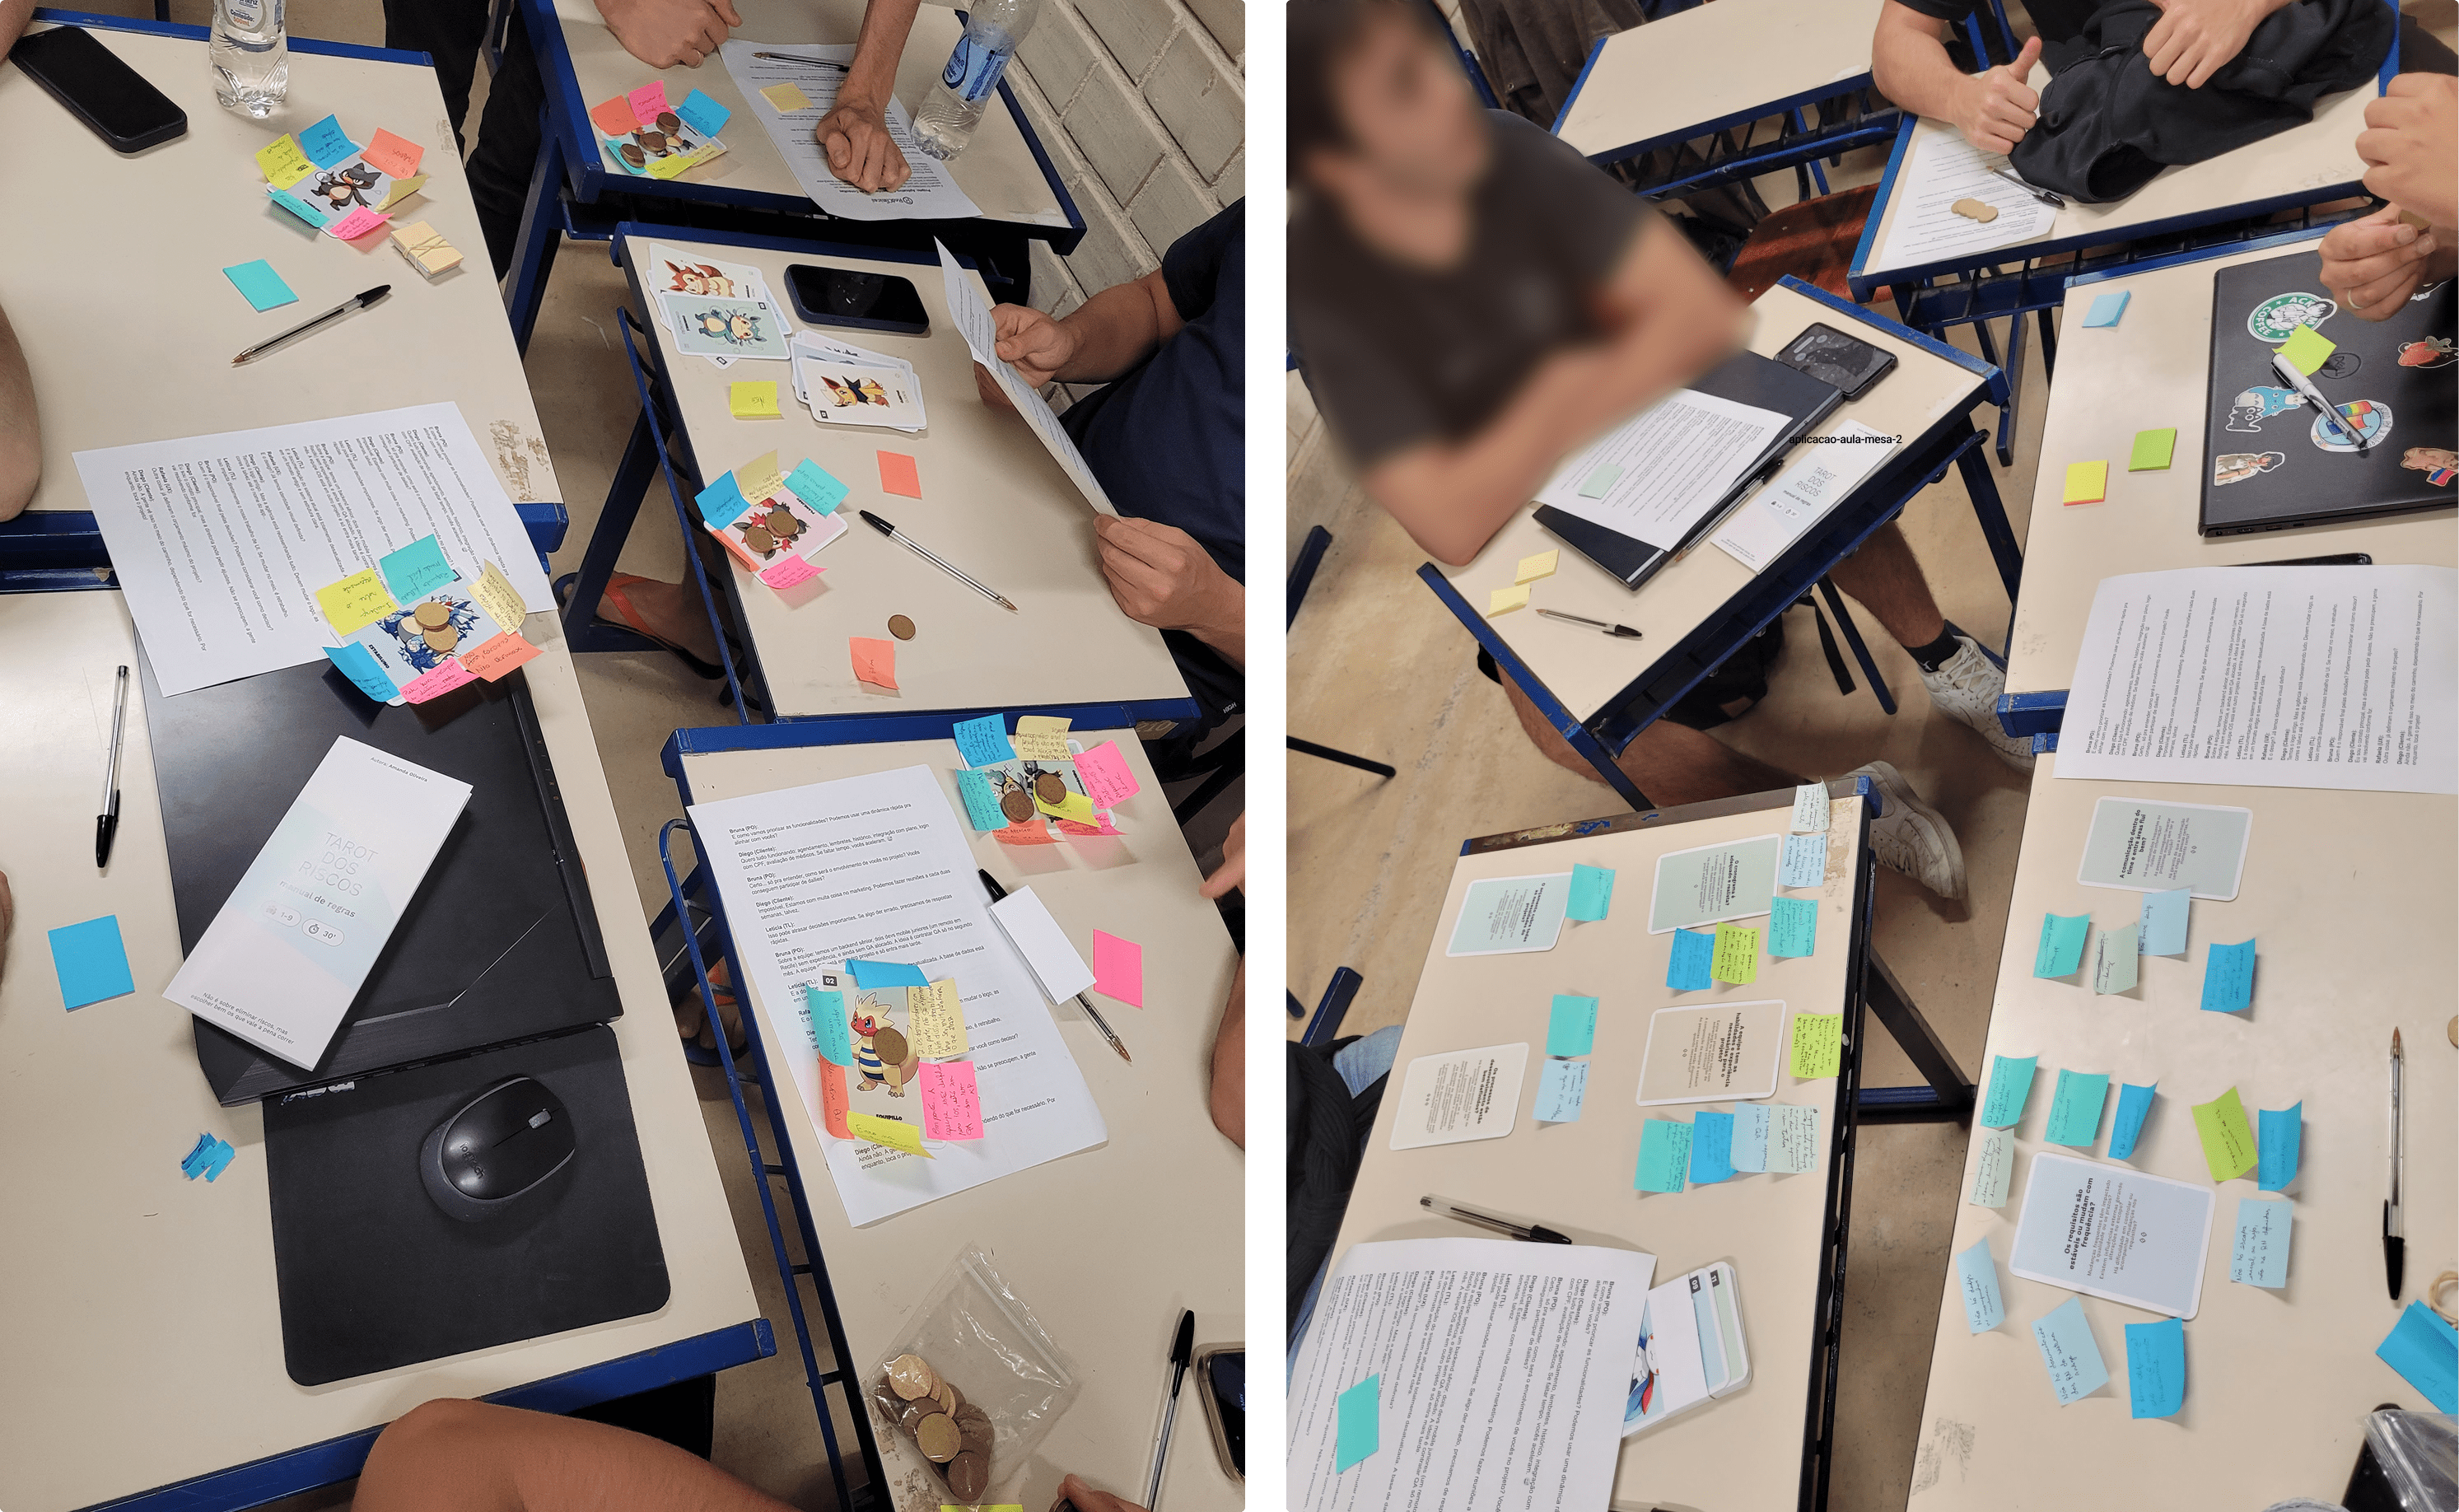
\includegraphics[width=0.8\textwidth]{aplicacao-aula-mesa-2}
	\legend{Fonte: Autora (2025)}
\end{figure}

\subsubsection{Análise dos dados coletados}

A análise dos dados coletados a partir dos questionários e da observação da execução com os estudantes permitiu avaliar indícios da eficácia da dinâmica na promoção da identificação de riscos relevantes e no estímulo às discussões. Primeiramente, é importante contextualizar o perfil dos participantes que contribuíram com a pesquisa.

No que tange às características demográficas dos participantes, a faixa etária predominante concentrou-se entre 18 e 28 anos, abrangendo 27 indivíduos. Um grupo menor, com 3 pessoas, situava-se na faixa de 29 a 39 anos. Em média, os estudantes tinham 23 anos.

Com relação à frequência com que os participantes costumam jogar jogos digitais, os dados coletados revelaram os seguintes hábitos: 10 pessoas jogam diariamente; 8 pessoas jogam semanalmente; 4 pessoas jogam mensalmente; e 8 pessoas jogam raramente, apenas de tempos em tempos.

Quanto à frequência de jogos não-digitais (de cartas, tabuleiro, etc.), a maioria (19 pessoas) joga raramente, de tempos em tempos. Em seguida, 7 pessoas jogam mensalmente, e 4 pessoas jogam semanalmente. Estes dados fornecem um perfil sobre a familiaridade dos participantes com diferentes formatos de jogos, o que pode influenciar a receptividade a dinâmicas gamificadas.

Com base nos dados coletados dos participantes e na observação das atividades, os resultados da aplicação da dinâmica permitiram as análises descritas a seguir.

Não houve um consenso absoluto entre os riscos priorizados pelos diferentes grupos; no entanto, foi possível observar uma recorrência nos riscos mais votados, que se concentraram em categorias como cronograma (identificado por 75\% dos grupos) e comunicação (44\% dos grupos).

Em termos de quantidade de riscos, os grupos do período noturno avaliaram, em média, 8,2 riscos, enquanto os grupos do período matutino avaliaram, em média, 12,25 riscos, resultando em uma média geral de 10 riscos avaliados por grupo em aproximadamente 30 minutos. Esses resultados preliminares indicam que a dinâmica foi capaz de gerar um volume significativo de riscos e fomentar a discussão sobre os mesmos, o que é um indicativo positivo para a sua aplicabilidade.

Os dados obtidos por meio dos questionários preenchidos pelos estudantes foram consolidados e analisados conforme o formato proposto pelo modelo MEEGA+. A partir desses dados, foram gerados gráficos (a serem apresentados nas Figuras subsequentes) que possibilitam uma análise detalhada dos aspectos avaliados em relação à Usabilidade, Experiência do Jogador e às afirmativas específicas da dinâmica.

Em relação à avaliação da Usabilidade, a Figura \ref{ufsc-usabilidade} apresenta um gráfico consolidado com os resultados obtidos. É possível verificar que a dinâmica obteve resultados altamente positivos nesta categoria. Itens como atratividade visual, consistência de textos, cores e fontes, legibilidade e compreensão das cores obtiveram mediana 2 (Concordo fortemente). Esse insight reforça que o design é um ponto forte e unânime da dinâmica, sendo percebida como visual e funcionalmente atrativa, com uma apresentação clara e profissional que contribui positivamente para a imersão e uma boa primeira impressão entre os estudantes. No tópico de Usabilidade, a afirmativa  “Eu precisei aprender poucas coisas para poder começar a jogar” obteve a menor mediana geral, com 50\% dos participantes concordando ou concordando fortemente, 40\% indiferentes e 10\% discordantes. Esses dados indicam que, embora o formato atual da gamificação tenha se mostrado efetivo para engajar uma parcela dos participantes, uma simplificação adicional no processo nas regras pode ser benéfica para alcançar maior satisfação em um grupo mais amplo.

\begin{figure}[H]
	\caption{\label{ufsc-usabilidade} Resultados da avaliação de usabilidade com estudantes}
  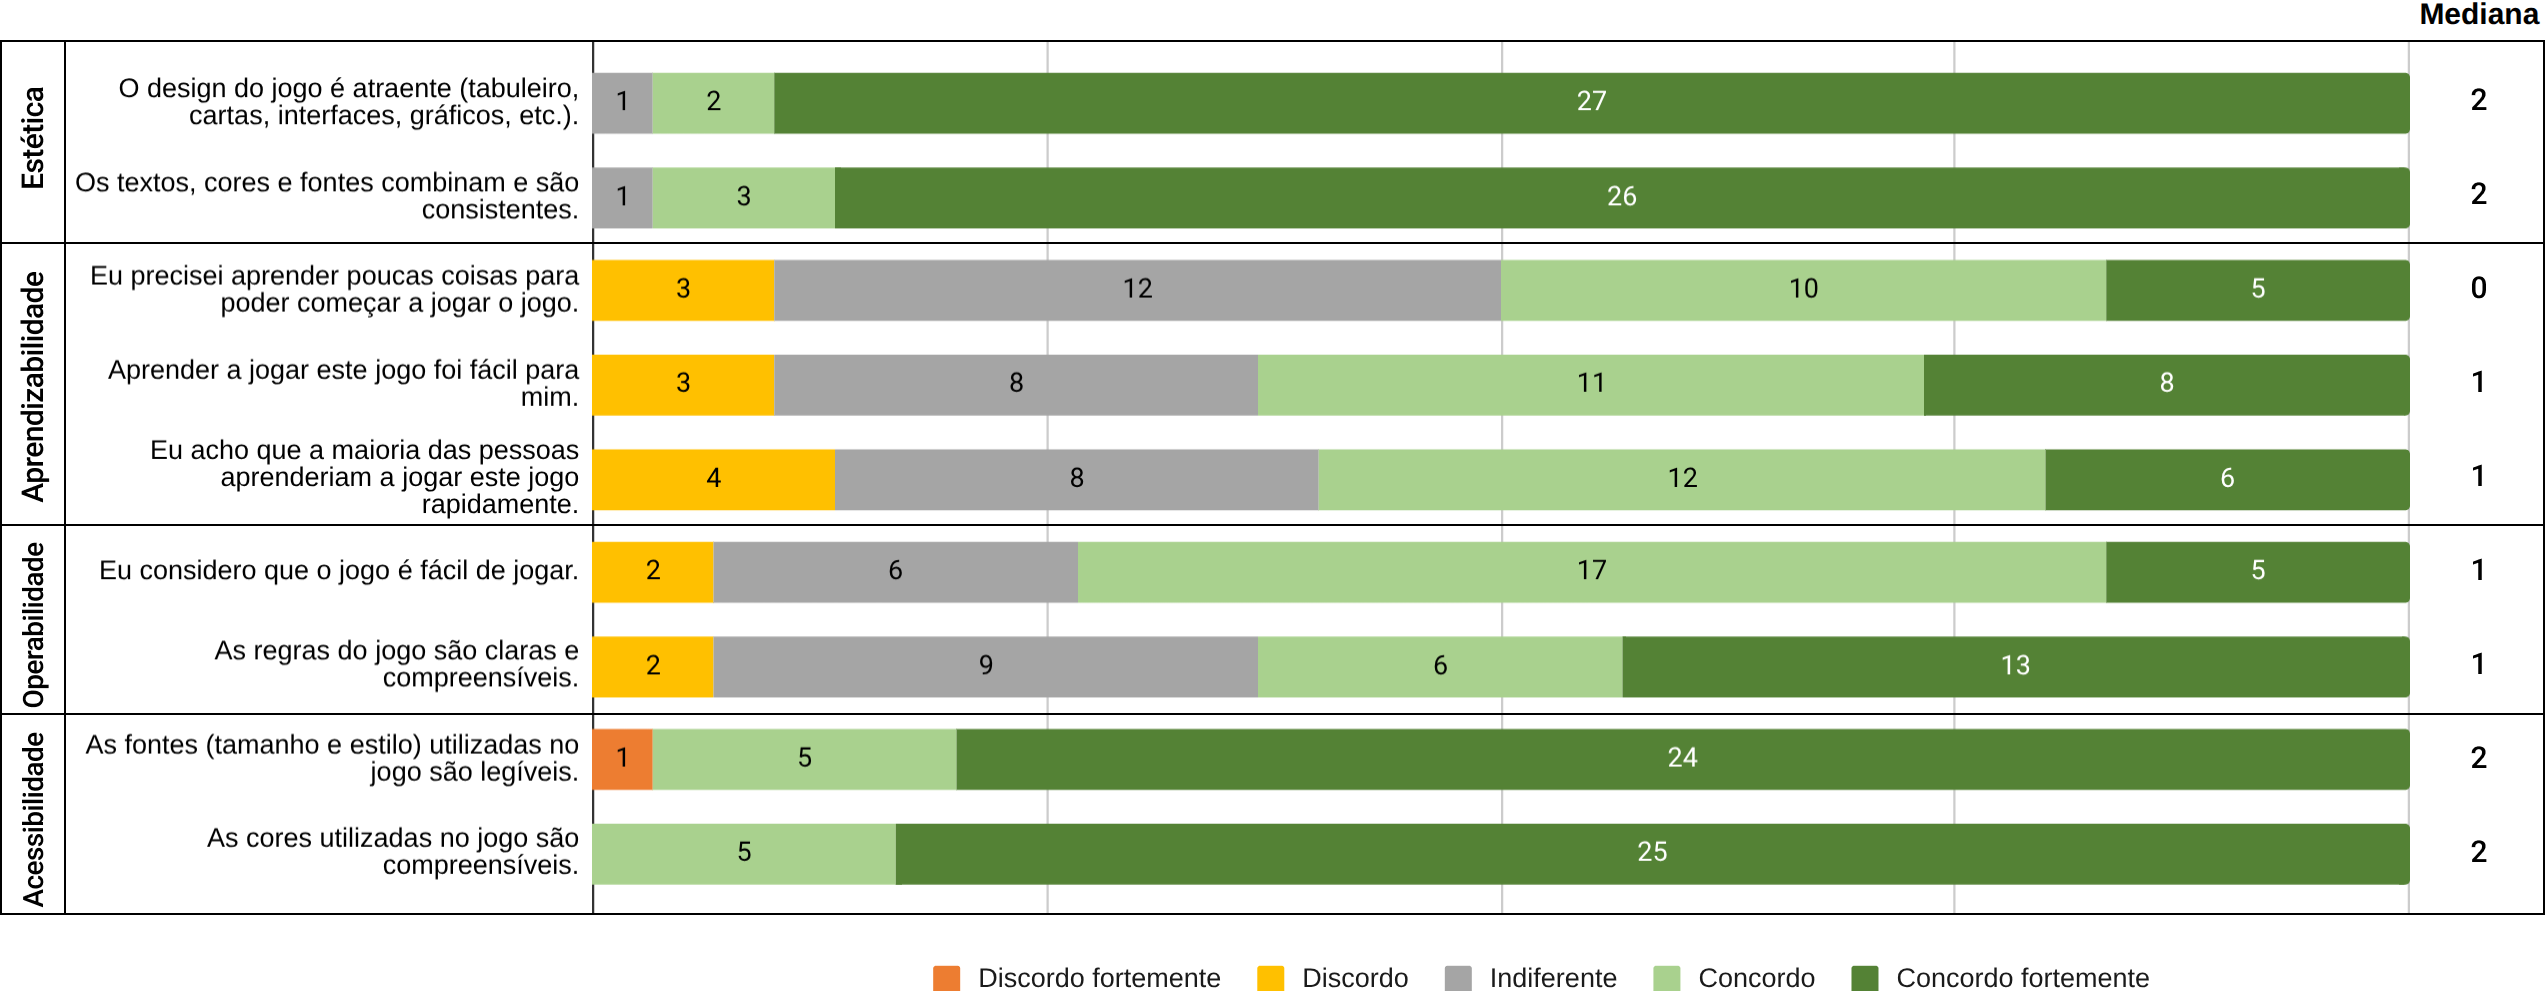
\includegraphics[width=\textwidth]{ufsc-usabilidade}
	\legend{Fonte: Autora (2025)}
\end{figure}

No critério Experiência do Jogador, a Figura \ref{ufsc-xp-jogador} ilustra os resultados obtidos. No que engloba a curva de aprendizado, clareza das regras e facilidade de jogar, observou-se que a mediana foi 1 (Concordo) em quase todos os itens. É importante notar uma dispersão significativa nas respostas, com a ocorrência de vários votos em -1 (Discordo), 0 (Indiferente) e até alguns em -2 (Discordo fortemente). Esse insight indica que os estudantes perceberam uma maior dificuldade para aprender a jogar e compreender as regras inicialmente. Isso sugere que o processo de onboarding e a explicação da dinâmica necessitam de ajustes para o contexto educacional, talvez com a inclusão de uma rodada de exemplo ou um vídeo instrutivo pré-aplicação para minimizar o tempo de adaptação e as dúvidas iniciais.

\begin{figure}[H]
	\caption{\label{ufsc-xp-jogador} Resultados da avaliação de experiência do jogador com estudantes}
  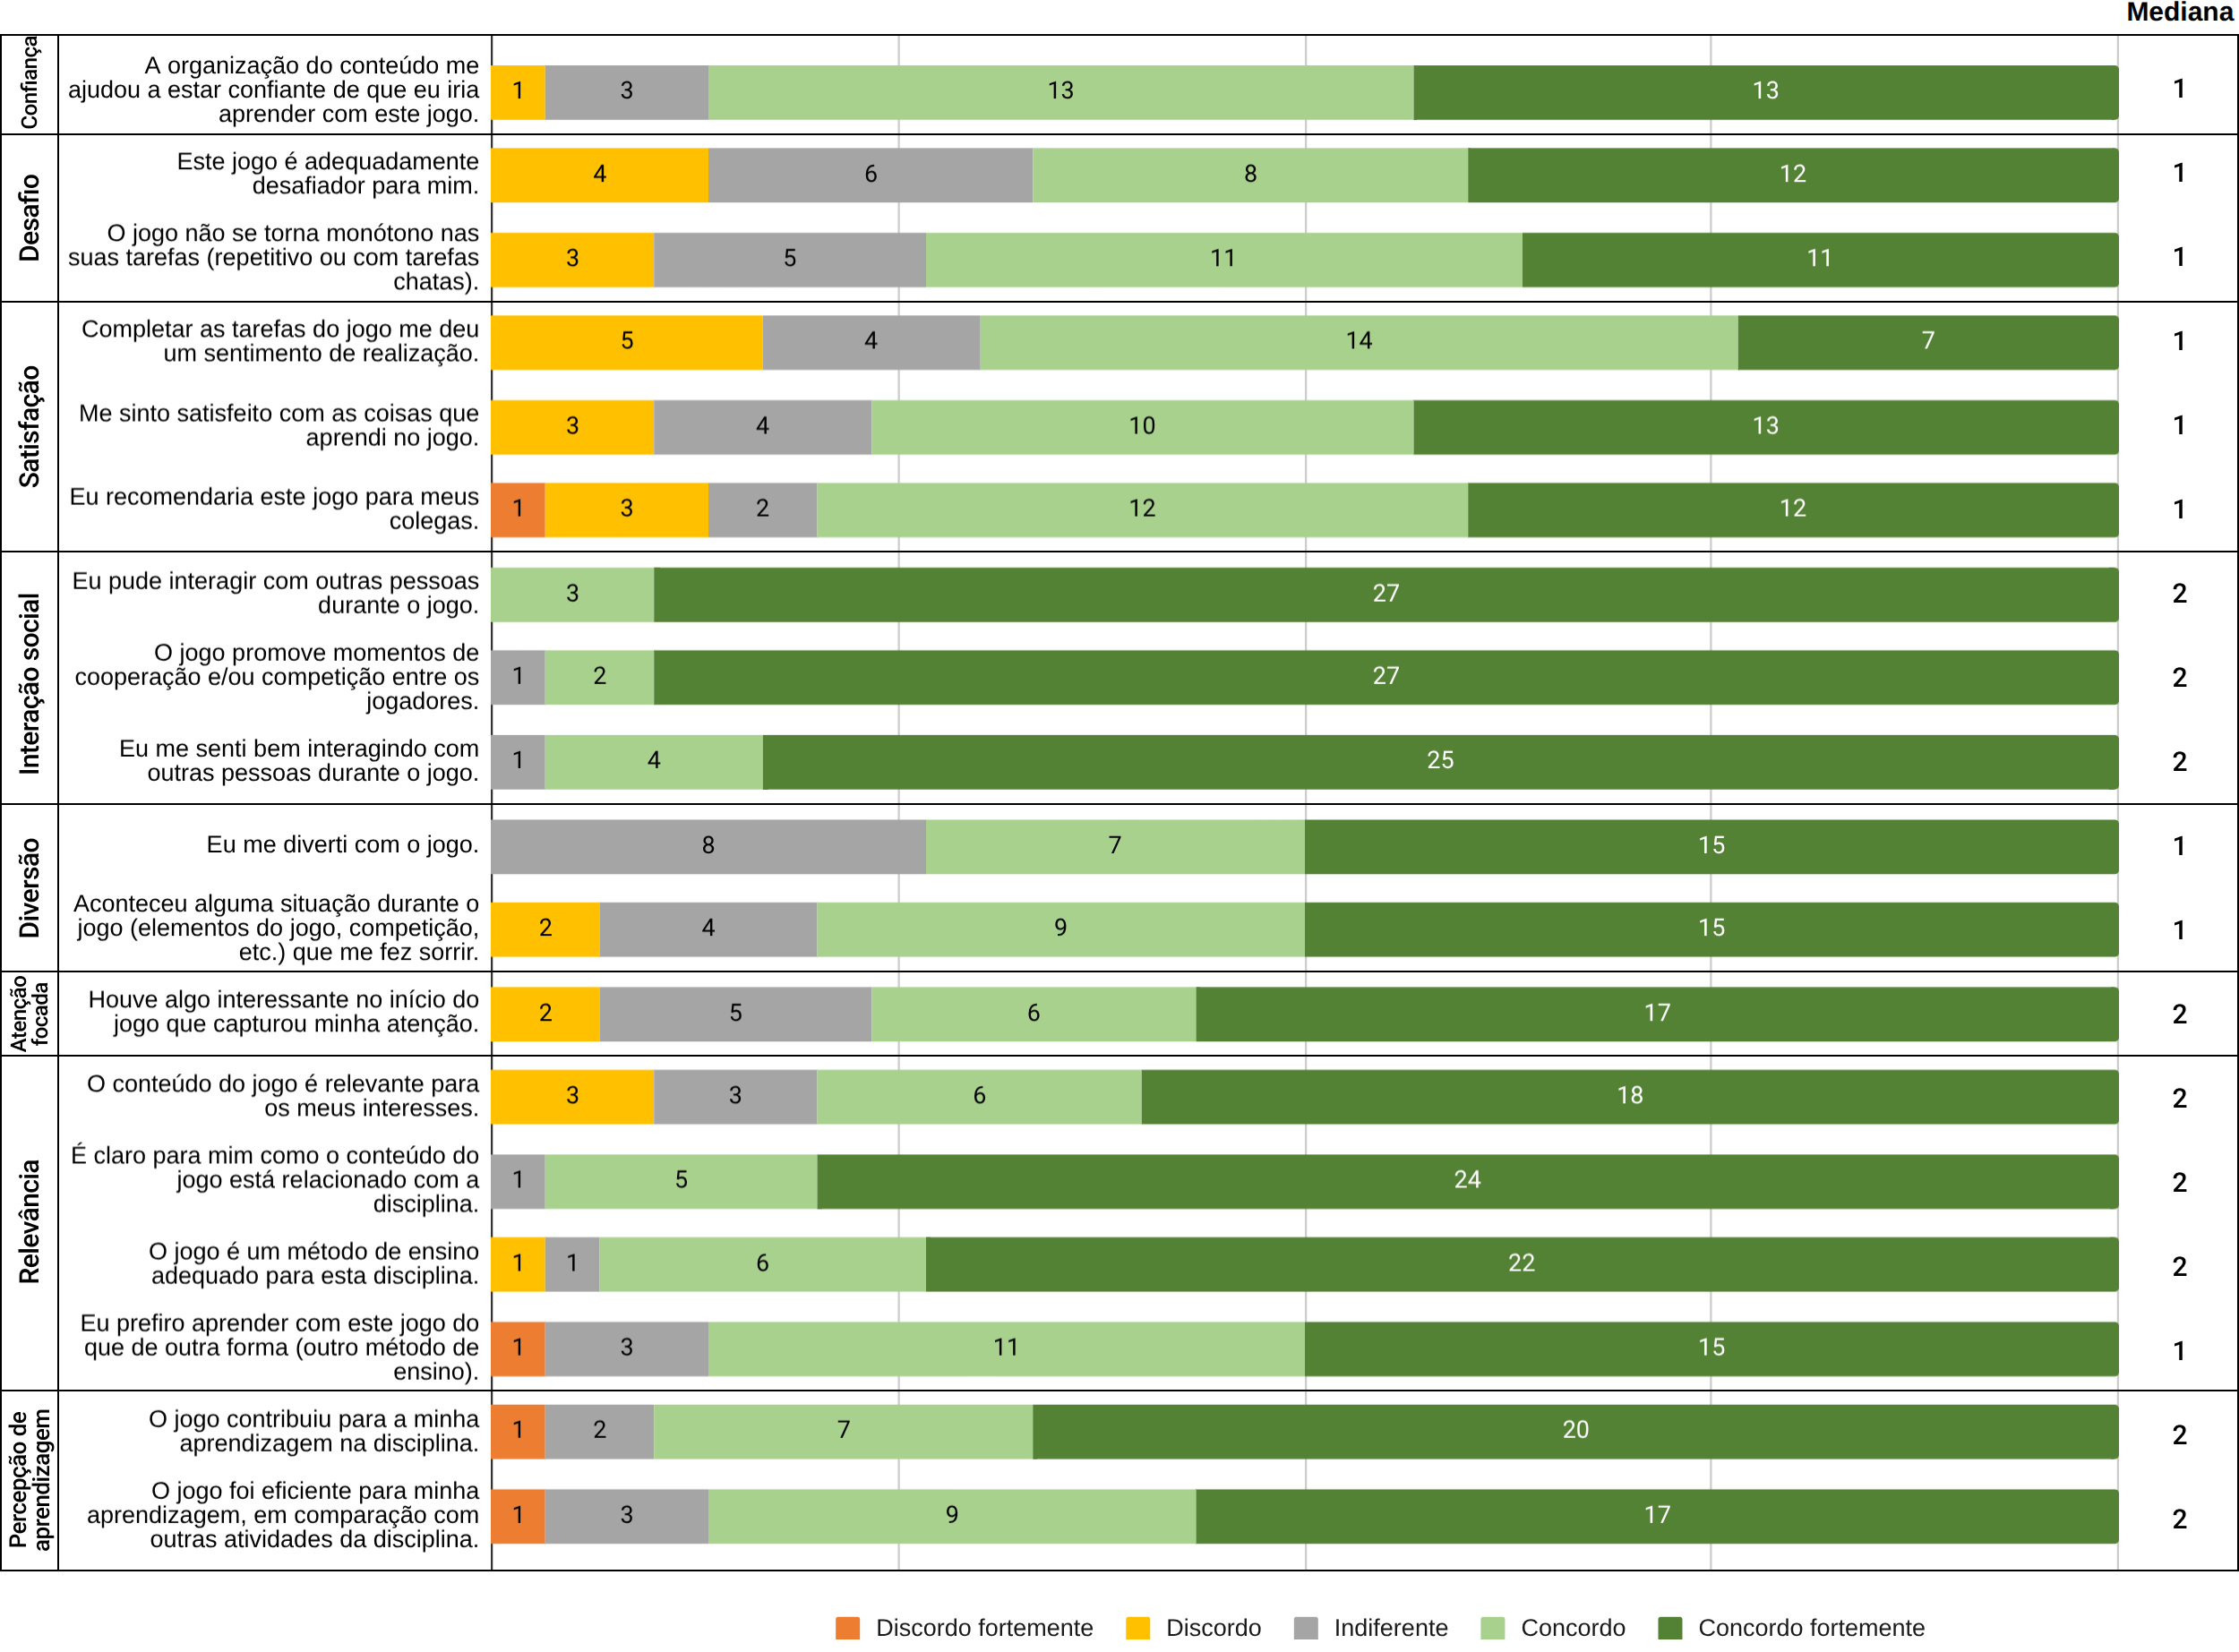
\includegraphics[width=\textwidth]{ufsc-xp-jogador}
	\legend{Fonte: Autora (2025)}
\end{figure}

Em relação à dinâmica e envolvimento, que analisa aspectos como desafio adequado, não-monotonia e sentimento de realização, os resultados apresentaram mediana 1 (Concordo) para a maioria desses itens. A análise da distribuição das respostas revela alguns votos negativos e uma concentração em valores medianos (0 e 1), indicando que, embora a dinâmica não seja percebida como entediante, ela não gerou um forte senso de desafio ou conquista entre os estudantes. Isso pode apontar para um desequilíbrio entre a simplicidade da dinâmica e o estímulo esperado, que talvez aguardasse uma experiência mais  “gamificada” ou competitiva. Há, portanto, espaço para evoluir as mecânicas ou introduzir mais variações nas atividades para potencializar o engajamento emocional.

A dimensão da interação social foi avaliada com mediana 2 (Concordo fortemente) em todos os seus itens, incluindo interação com outras pessoas, cooperação/competição e sentimento positivo ao interagir. Essa é uma força notável da dinâmica, pois indica que, mesmo em um ambiente de sala de aula, houve um forte engajamento e conexão entre os colegas. Isso é excelente para promover habilidades interpessoais, trabalho em grupo e a comunicação eficaz, elementos cruciais no desenvolvimento de projetos.

Nos itens relacionados ao engajamento e diversão, como  “Me diverti com o jogo”,  “Senti vontade de sorrir” e  “Me capturou no início”, a mediana foi 1 (Concordo), e foi observada uma maior dispersão nas respostas. Esse insight sugere que, apesar da clareza visual e das boas interações sociais, o fator  “diversão” teve uma intensidade moderada. Isso pode ser influenciado pelo ambiente de sala de aula ou pela não familiaridade dos participantes uns com os outros, que pode inibir o engajamento espontâneo. A introdução de elementos mais lúdicos, a promoção de um ambiente mais descontraído, ou a alocação de mais tempo livre para a exploração da dinâmica pode contribuir para aumentar o prazer e a imersão.

A conexão com o conteúdo pedagógico foi um ponto de destaque. Todos os itens relacionados a esta categoria, como clareza da relação com a disciplina, aprendizagem com o jogo, relevância e comparação positiva com outros métodos, obtiveram mediana 2 (Concordo fortemente). Esse resultado demonstra que a dinâmica cumpre bem seus objetivos pedagógicos, sendo reconhecida pelos estudantes como eficaz, aplicável e, em muitos casos, preferível a outros métodos tradicionais de ensino sobre gestão de riscos. Este é um grande diferencial didático da ferramenta.

Finalmente, para as afirmativas customizadas e específicas da dinâmica, a Figura \ref{ufsc-afirmativas} apresenta os resultados. Todos os itens da seção obtiveram mediana 2 (Concordo fortemente), indicando que a dinâmica é bem-sucedida em despertar a consciência sobre riscos em projetos, sendo efetiva em promover a identificação e discussão desses elementos mesmo com um público acadêmico.

\begin{figure}[H]
	\caption{\label{ufsc-afirmativas} Resultados da avaliação de afirmativas específicas com estudantes}
  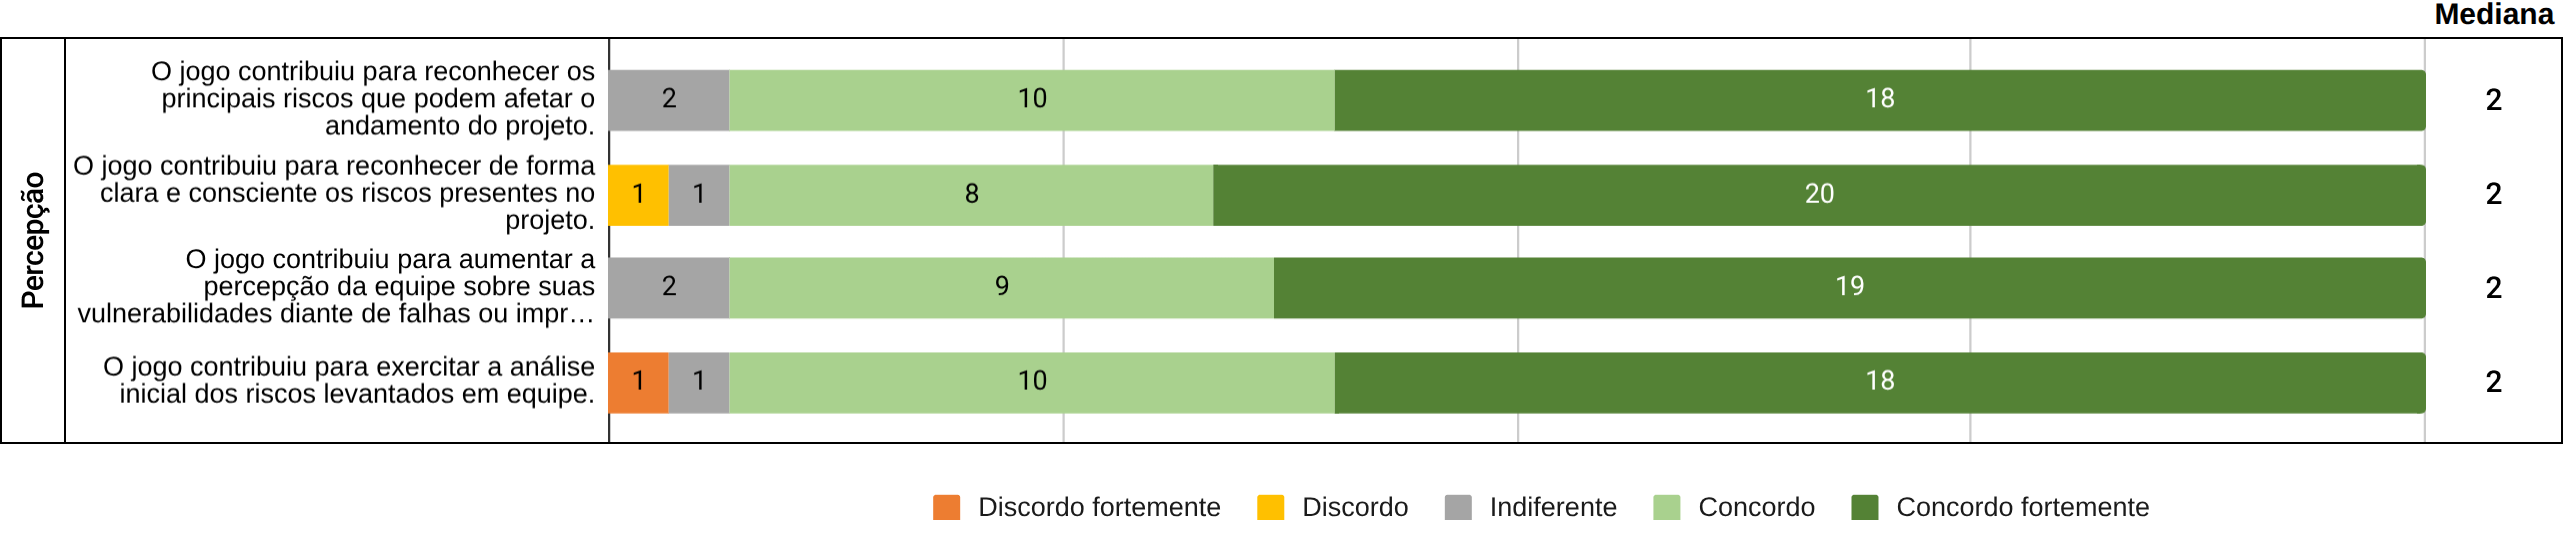
\includegraphics[width=\textwidth]{ufsc-afirmativas}
	\legend{Fonte: Autora (2025)}
\end{figure}

Além dos dados quantitativos, a coleta de \textit{feedback} aberto revelou percepções valiosas dos estudantes sobre a dinâmica. Os pontos mais elogiados incluíram:
\begin{itemize}
  \item \textbf{Qualidade e estética do material}: O design atrativo das cartas e a qualidade do material foram frequentemente mencionados, contribuindo para uma experiência visualmente agradável.
  \item \textbf{Interatividade e colaboração}: A dinâmica promoveu a interação e discussão em equipe, sendo destacada como um facilitador para a troca de ideias e a classificação colaborativa de riscos.
  \item \textbf{Eficácia na identificação e análise de riscos}: Muitos participantes apontaram a capacidade da dinâmica em auxiliar na identificação e análise inicial de riscos, mesmo com diferentes interpretações de uma mesma carta.
  \item \textbf{Abordagem descontraída}: A maneira lúdica e descontraída de abordar um tema complexo como riscos foi bem recebida, tornando o aprendizado mais engajador.
\end{itemize}

Quanto aos aspectos que poderiam ser melhorados, as sugestões dos participantes focaram em:
\begin{itemize}
  \item \textbf{Número e repetitividade das cartas}: Alguns estudantes sentiram que o número de cartas era excessivo ou que algumas apresentavam temáticas muito similares/sobrepostas, o que poderia levar a respostas parecidas ou não agregar valor suficiente.
  \item \textbf{Clareza das regras e tempo}: Sugeriu-se que as regras poderiam ser mais claras e que o tempo de execução, especialmente da primeira etapa, poderia ser estendido para permitir uma leitura e discussão mais aprofundada. A ideia de um exemplo prático ou vídeo explicativo foi mencionada para facilitar o entendimento inicial.
  \item \textbf{Estruturação da análise}: Houve sugestões para padronizar a forma de registrar os riscos (um \textit{post-it} por risco) e, em alguns casos, para uma organização das cartas (ex.: diagrama de Ishikawa) que pudesse guiar a identificação de riscos de forma mais estruturada.
  \item \textbf{Detalhes do cenário}: Alguns participantes sugeriram que o caso de projeto fictício poderia ser mais detalhado ou que a dinâmica poderia exemplificar melhor o que considerar como risco.
\end{itemize}

Essas percepções qualitativas complementam os dados quantitativos, oferecendo insights importantes para a evolução e aprimoramento contínuo da dinâmica.

\subsection{Avaliação com profissionais}

Após a avaliação inicial conduzida com estudantes, uma segunda etapa da avaliação foi realizada com profissionais atuantes no mercado de tecnologia, visando obter \textit{feedback} de um público com experiência prática em ambientes de desenvolvimento ágil. Nesta avaliação, também foi empregado o questionário do MEEGA+ adaptado, com o objetivo de avaliar a dinâmica de gamificação para a identificação e análise de riscos em equipes ágeis.

A aplicação ocorreu no contexto do Laboratório Bridge da UFSC, um ambiente focado em pesquisa e desenvolvimento de \textit{software}, com ênfase em inovação e soluções tecnológicas com compromisso social, com a devida autorização para realização da pesquisa, conforme detalhado no Anexo \ref{anexo:declaracao-concordancia}.

Fizeram parte dessa avaliação 6 equipes de desenvolvimento ágil voluntárias, pertencentes a 2 projetos distintos do Laboratório Bridge, totalizando 43 participantes. Os participantes são profissionais experientes no mercado de tecnologia, com atuação em desenvolvimento ágil e gestão de projetos, incluindo cargos como \textit{Scrum Master}, \textit{Product Owner}, programador, \textit{tester} e \textit{designer}, variando de acordo com a configuração de cada equipe. A distribuição dos participantes por papel pode ser observada na Tabela \ref{tab:participantes-papel}.

\begin{table}[H]
  \centering
  \caption{\label{tab:participantes-papel} Quantidade de participantes por papel}
  \begin{tabular}{|p{7cm}|p{2.5cm}|}
    \hline
    \textbf{Papel} & \textbf{Quantidade} \\
    \hline
    \textit{Scrum Master} & 6 \\
    \hline
    \textit{Product Owner} e Analista de sistemas & 7 \\
    \hline
    \textit{Developers} (Programadores e \textit{Testers}) & 26 \\
    \hline
    \textit{Designers} & 4 \\
    \hline
  \end{tabular}
  \legend{Fonte: Autora (2025)}
\end{table}

A aplicação da dinâmica foi conduzida pelos \textit{Scrum Masters (SMs)} responsáveis pelas equipes, sem a participação direta da autora do trabalho durante a execução, com exceção da aplicação realizada na equipe da própria autora. Todas as equipes utilizaram o modelo digital/remoto da dinâmica, aproveitando plataformas de uso diário como Google Meet e Discord e o quadro colaborativo digital no \textit{FigJam} para realizar a interação entre os participantes.

O procedimento para a realização da dinâmica no laboratório envolveu as seguintes etapas:
\begin{enumerate}
  \item \textbf{Explanação inicial}: Apresentação da dinâmica e seus objetivos para os \textit{SMs} das equipes do laboratório Bridge, a fim de despertar o interesse e obter voluntários.
  \item \textbf{Reunião de alinhamento com \textit{SMs}}: Para as equipes interessadas, foi realizada uma reunião de 30 minutos com os \textit{SMs} responsáveis. Nesta reunião, a dinâmica foi explicada em detalhes, assim como os objetivos da aplicação e as diretrizes para sua condução.
  \item \textbf{Aplicação autônoma pelas equipes}: Os \textit{SMs} foram então orientados a aplicar a dinâmica com suas respectivas equipes, seguindo as regras e etapas previamente definidas.
  \item \textbf{Coleta de dados}: Após a aplicação, os participantes foram convidados a responder o questionário do MEEGA+ adaptado. Foram obtidas 35 respostas ao questionário, representando um retorno de 81,4\% dos participantes.
\end{enumerate}

\begin{figure}[H]
  \centering
	\caption{\label{bridge-print-quadro-1} Organização do quadro pelos profissionais 01}
  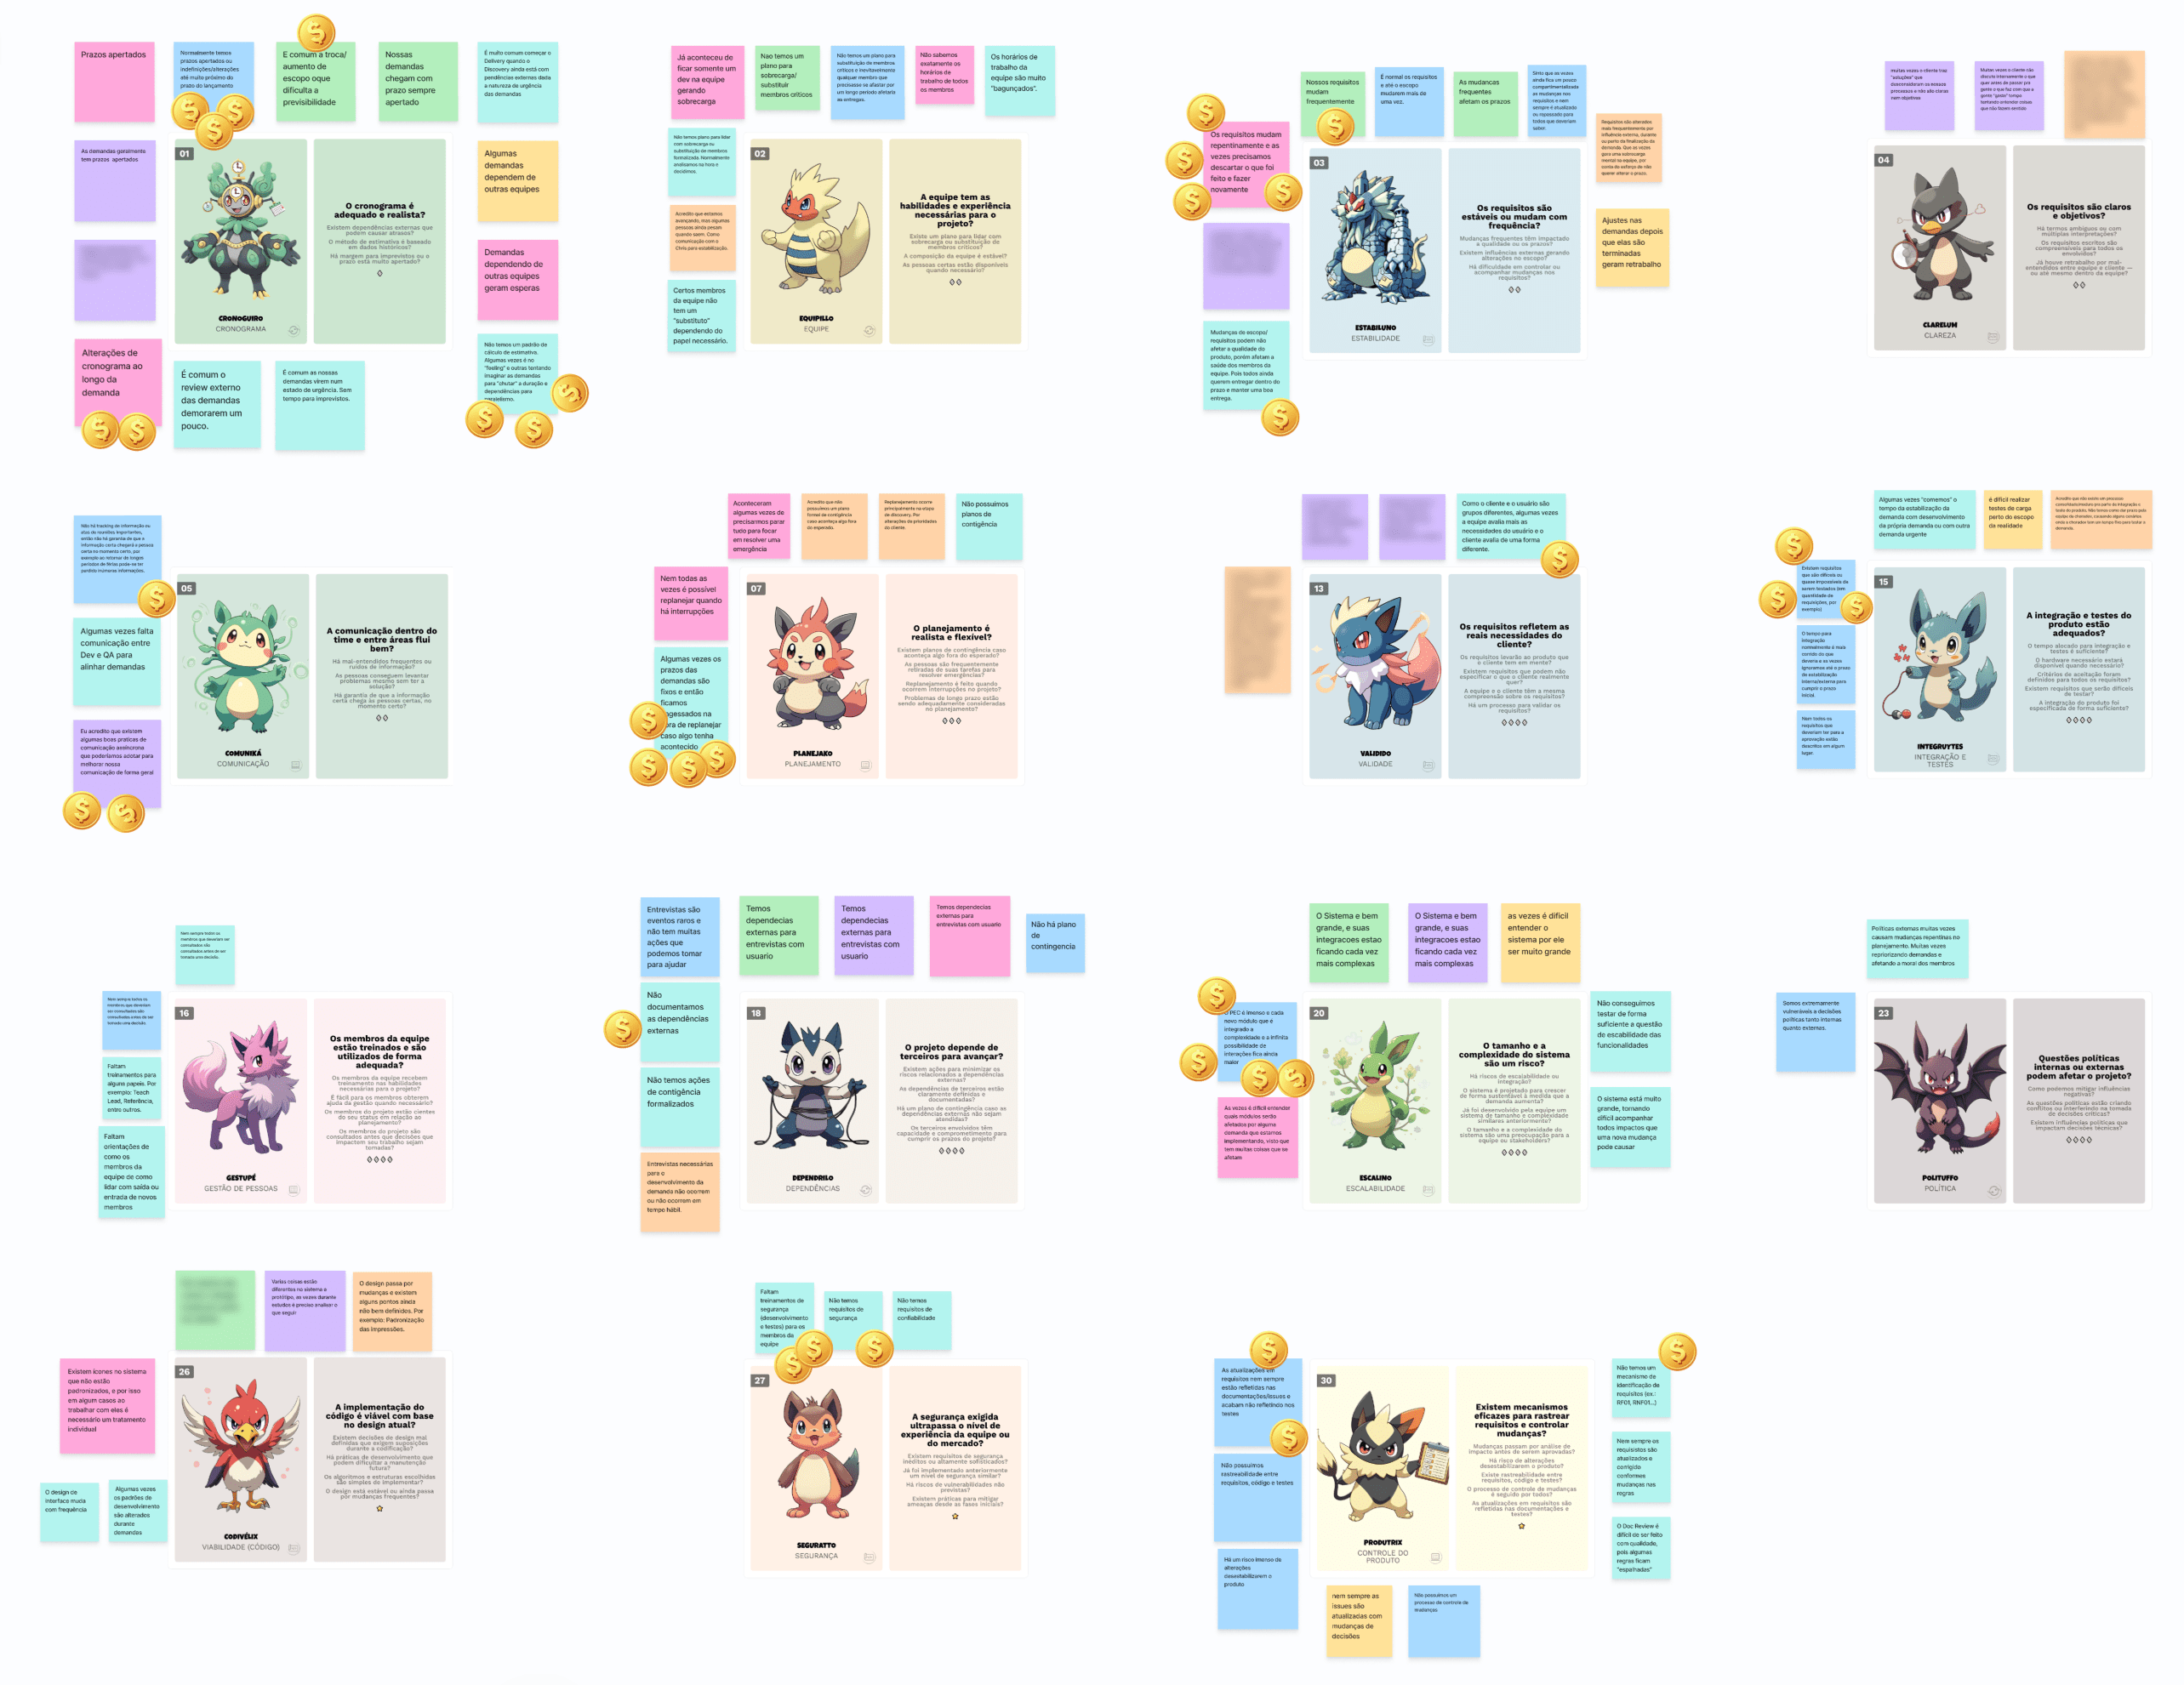
\includegraphics[width=0.8\textwidth]{bridge-print-quadro-1}
	\legend{Fonte: Autora (2025)}
\end{figure}

\begin{figure}[H]
  \centering
	\caption{\label{bridge-print-quadro-2} Organização do quadro pelos profissionais 02}
  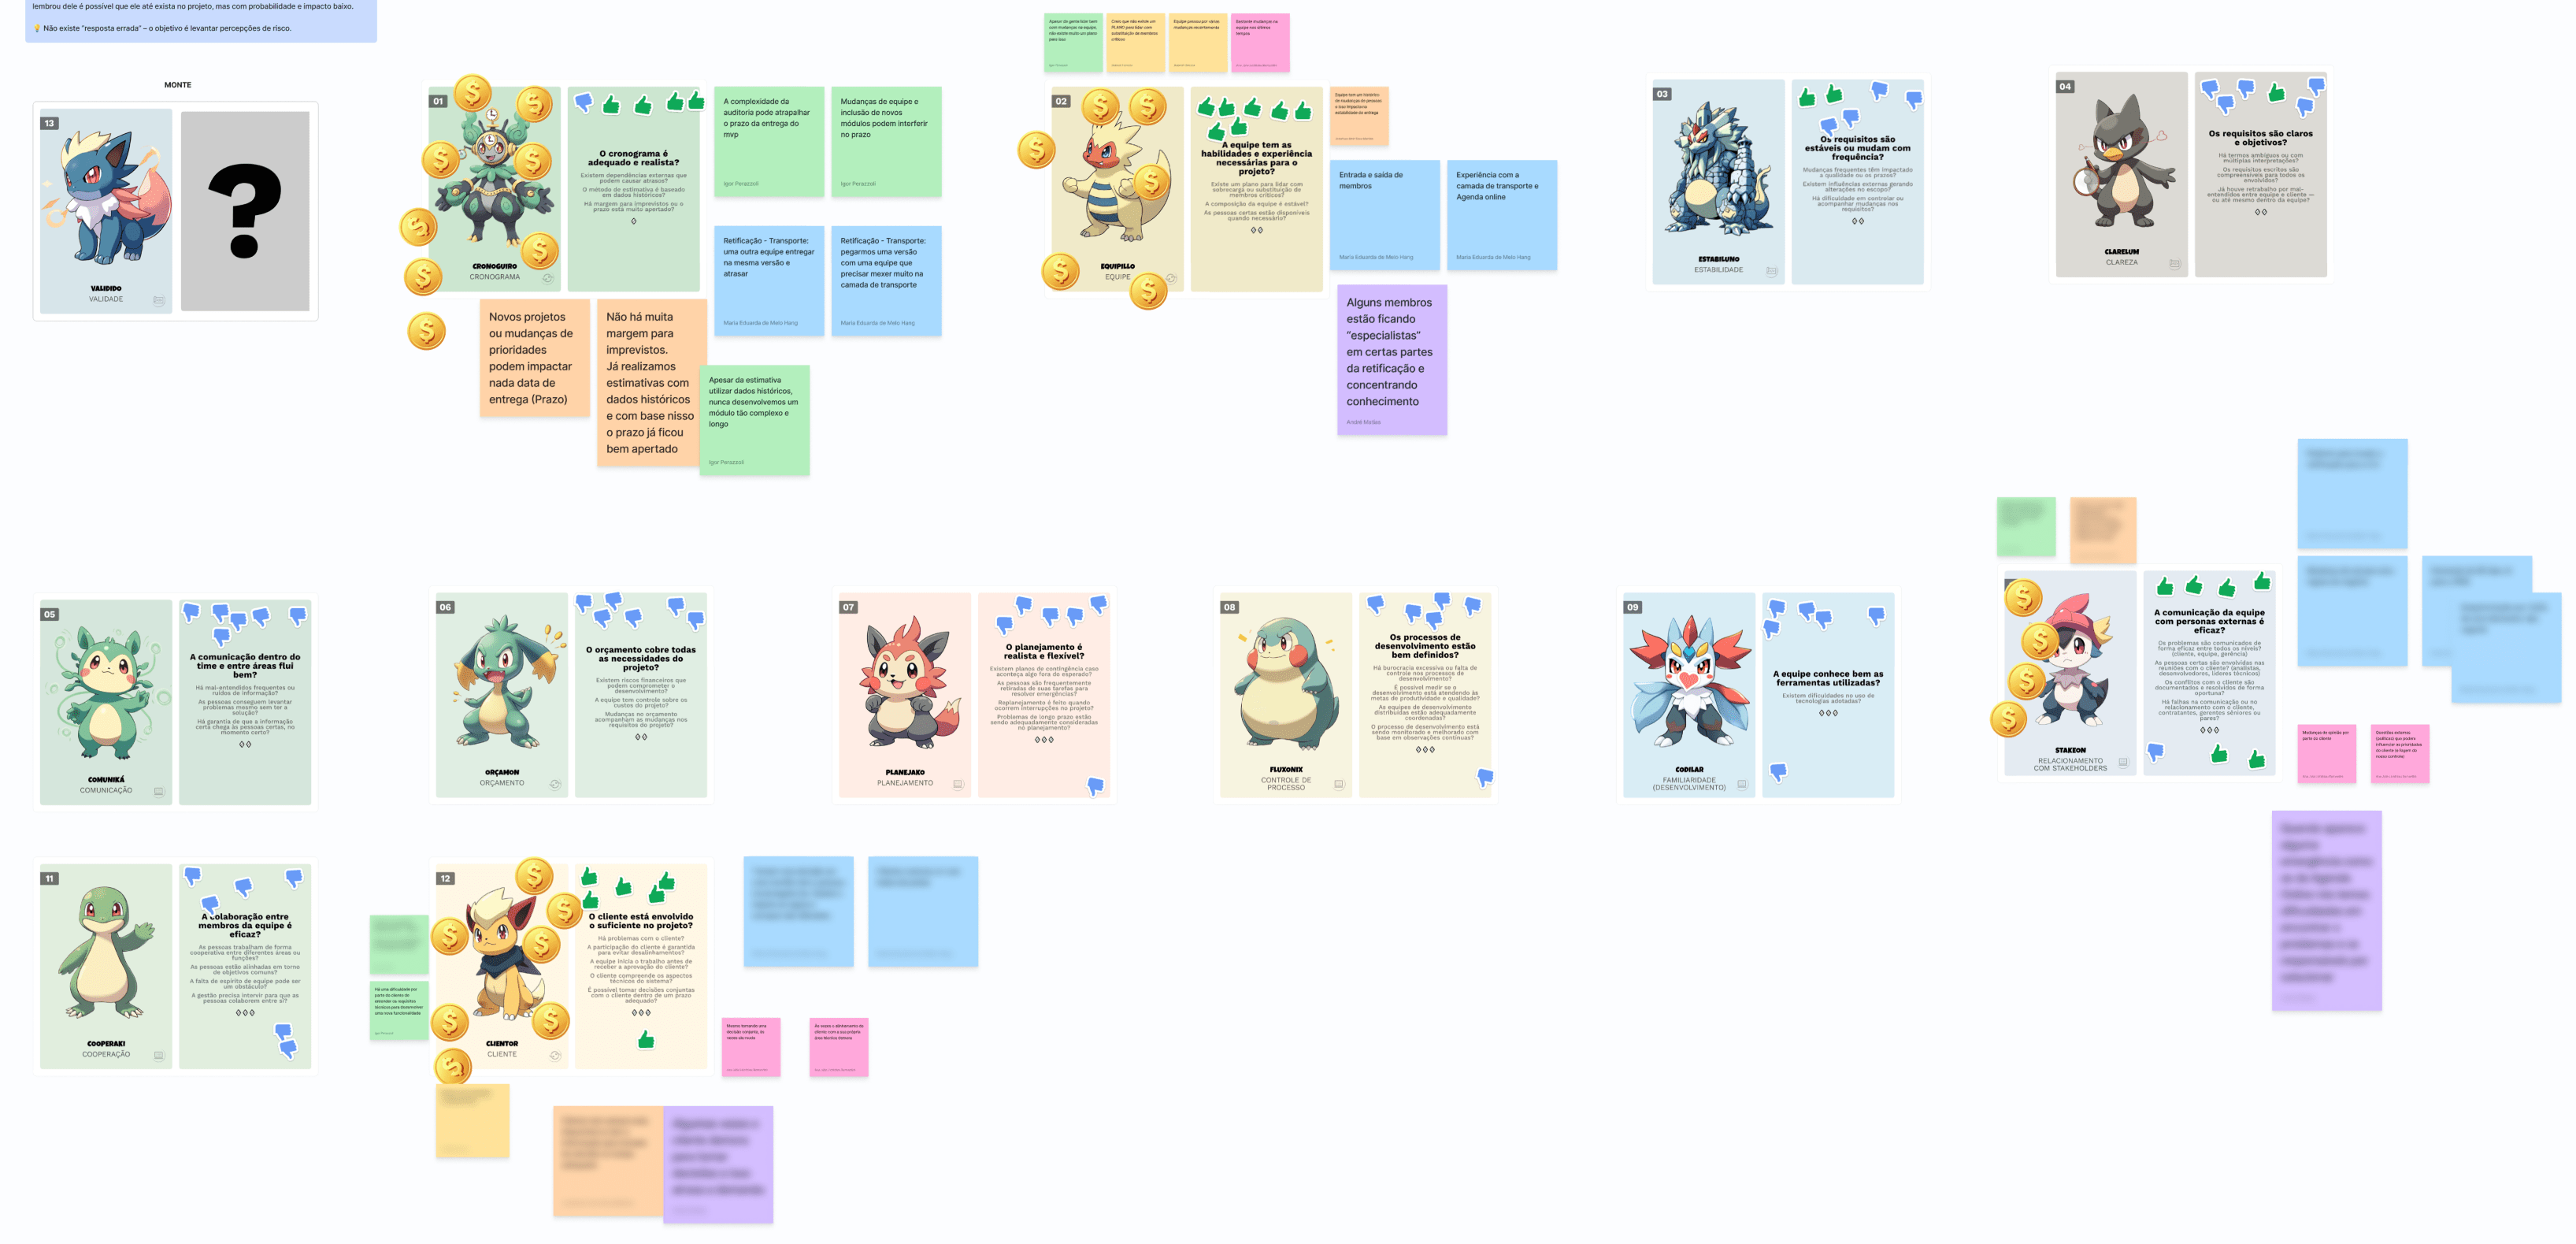
\includegraphics[width=0.8\textwidth]{bridge-print-quadro-2}
	\legend{Fonte: Autora (2025)}
\end{figure}

\begin{figure}[H]
  \centering
	\caption{\label{bridge-print-quadro-3} Organização do quadro pelos profissionais 03}
  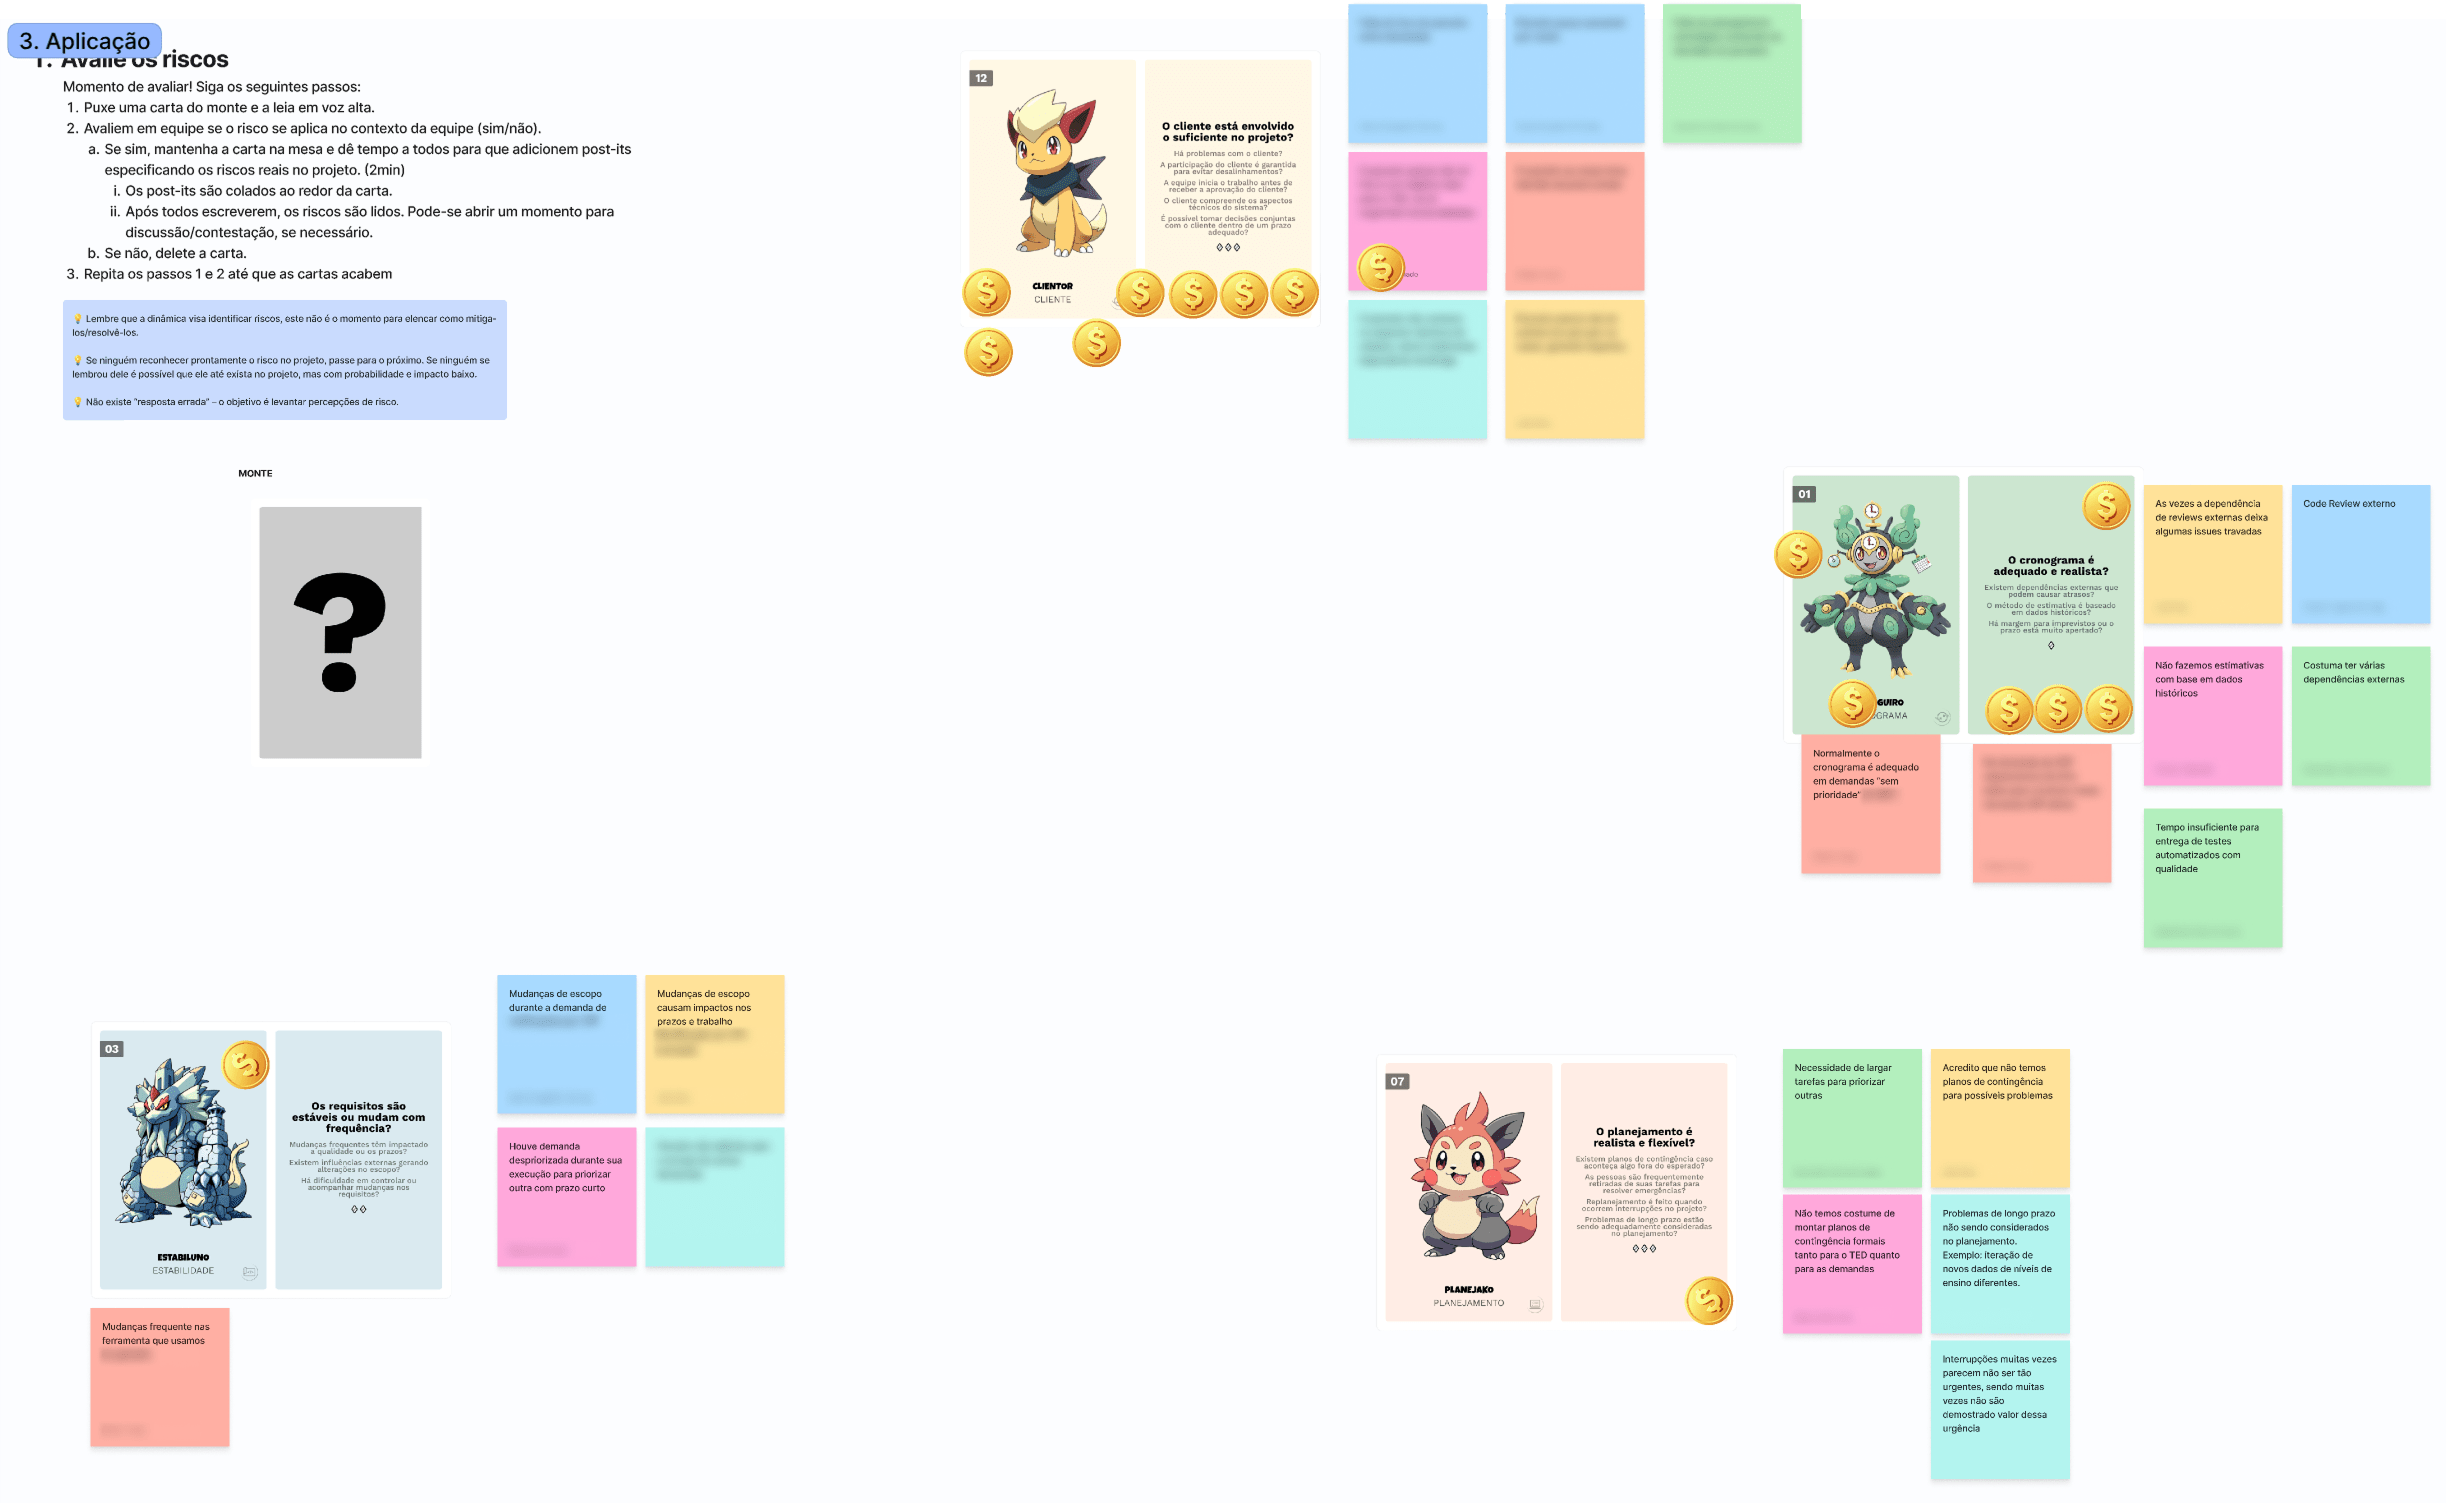
\includegraphics[width=0.8\textwidth]{bridge-print-quadro-3}
	\legend{Fonte: Autora (2025)}
\end{figure}

Durante as aplicações, observaram-se algumas variações relevantes que caracterizam o contexto de uso da dinâmica:
\begin{itemize}
  \item A quantidade de participantes por aplicação variou entre 7 e 8 integrantes por equipe.
  \item Quanto ao material utilizado, duas equipes aplicaram o sub-deck básico de cartas, três equipes aplicaram o deck completo, e uma equipe utilizou um sub-deck customizado de 17 cartas.
  \item O tempo médio de aplicação também variou conforme o deck utilizado: 63 minutos para o deck básico, 90 minutos para o deck completo, e 60 minutos para o sub-deck de 17 cartas.
  \item Em relação ao escopo da análise, metade das equipes realizou uma aplicação abrangente, enquanto a outra metade focou a dinâmica em riscos de próximas demandas com previsão de início de desenvolvimento iminente.
\end{itemize}

\subsubsection{Análise dos dados coletados}

A análise dos dados coletados a partir dos questionários e das observações das aplicações com profissionais forneceu insights valiosos sobre a aplicabilidade e percepção da dinâmica em um ambiente de trabalho real. Primeiramente, é fundamental apresentar o perfil dos participantes que contribuíram com esta etapa da pesquisa.

No que tange às características demográficas dos profissionais participantes, a faixa etária predominante concentrou-se entre 18 e 28 anos, abrangendo 22 indivíduos. Um grupo significativo de 13 pessoas situava-se na faixa de 29 a 39 anos. A média de idade foi de 26 anos.

Com relação à frequência com que os participantes costumam jogar jogos digitais, os dados coletados revelaram os seguintes hábitos: 18 pessoas jogam semanalmente; 10 pessoas jogam raramente (de tempos em tempos); 4 pessoas jogam diariamente; 2 pessoas jogam mensalmente; e 1 pessoa nunca joga.

Quanto à frequência de jogos não-digitais (de cartas, tabuleiro, etc.), a maioria (15 pessoas) joga mensalmente. Em seguida, 11 pessoas jogam raramente (de tempos em tempos); 6 pessoas jogam semanalmente; e 1 pessoa nunca joga. Estes dados fornecem um perfil sobre a familiaridade dos profissionais com diferentes formatos de jogos, o que pode influenciar a sua receptividade a dinâmicas gamificadas.

Os dados obtidos por meio dos questionários foram consolidados no formato proposto pelo modelo MEEGA+ adaptado, permitindo a geração de gráficos para uma análise detalhada dos aspectos avaliados.

Em relação à Usabilidade, a Figura \ref{bridge-usabilidade} apresenta um gráfico consolidado com os resultados obtidos. É possível verificar que a proposta de gamificação obteve resultados bastante positivos neste critério. Todos os itens relacionados à aparência visual, combinação de cores e fontes, legibilidade e organização do conteúdo obtiveram mediana 2 (Concordo fortemente), indicando uma forte concordância dos participantes. Este resultado sugere que a dinâmica é percebida como visual e funcionalmente atrativa, com uma apresentação clara e profissional que contribui positivamente para a imersão e a primeira impressão. O item com o menor índice de aprovação, embora ainda elevado (88,5\% dos participantes concordaram), foi  “Eu precisei aprender poucas coisas para poder começar a jogar”. Isso indica que, apesar da alta usabilidade geral, uma simplificação adicional no processo de onboarding ou uma maior clareza nas instruções iniciais pode ser benéfica para otimizar a experiência inicial de todos os grupos, especialmente considerando a restrição de tempo em ambientes profissionais.

\begin{figure}[H]
	\caption{\label{bridge-usabilidade} Resultados da avaliação de usabilidade com profissionais}
  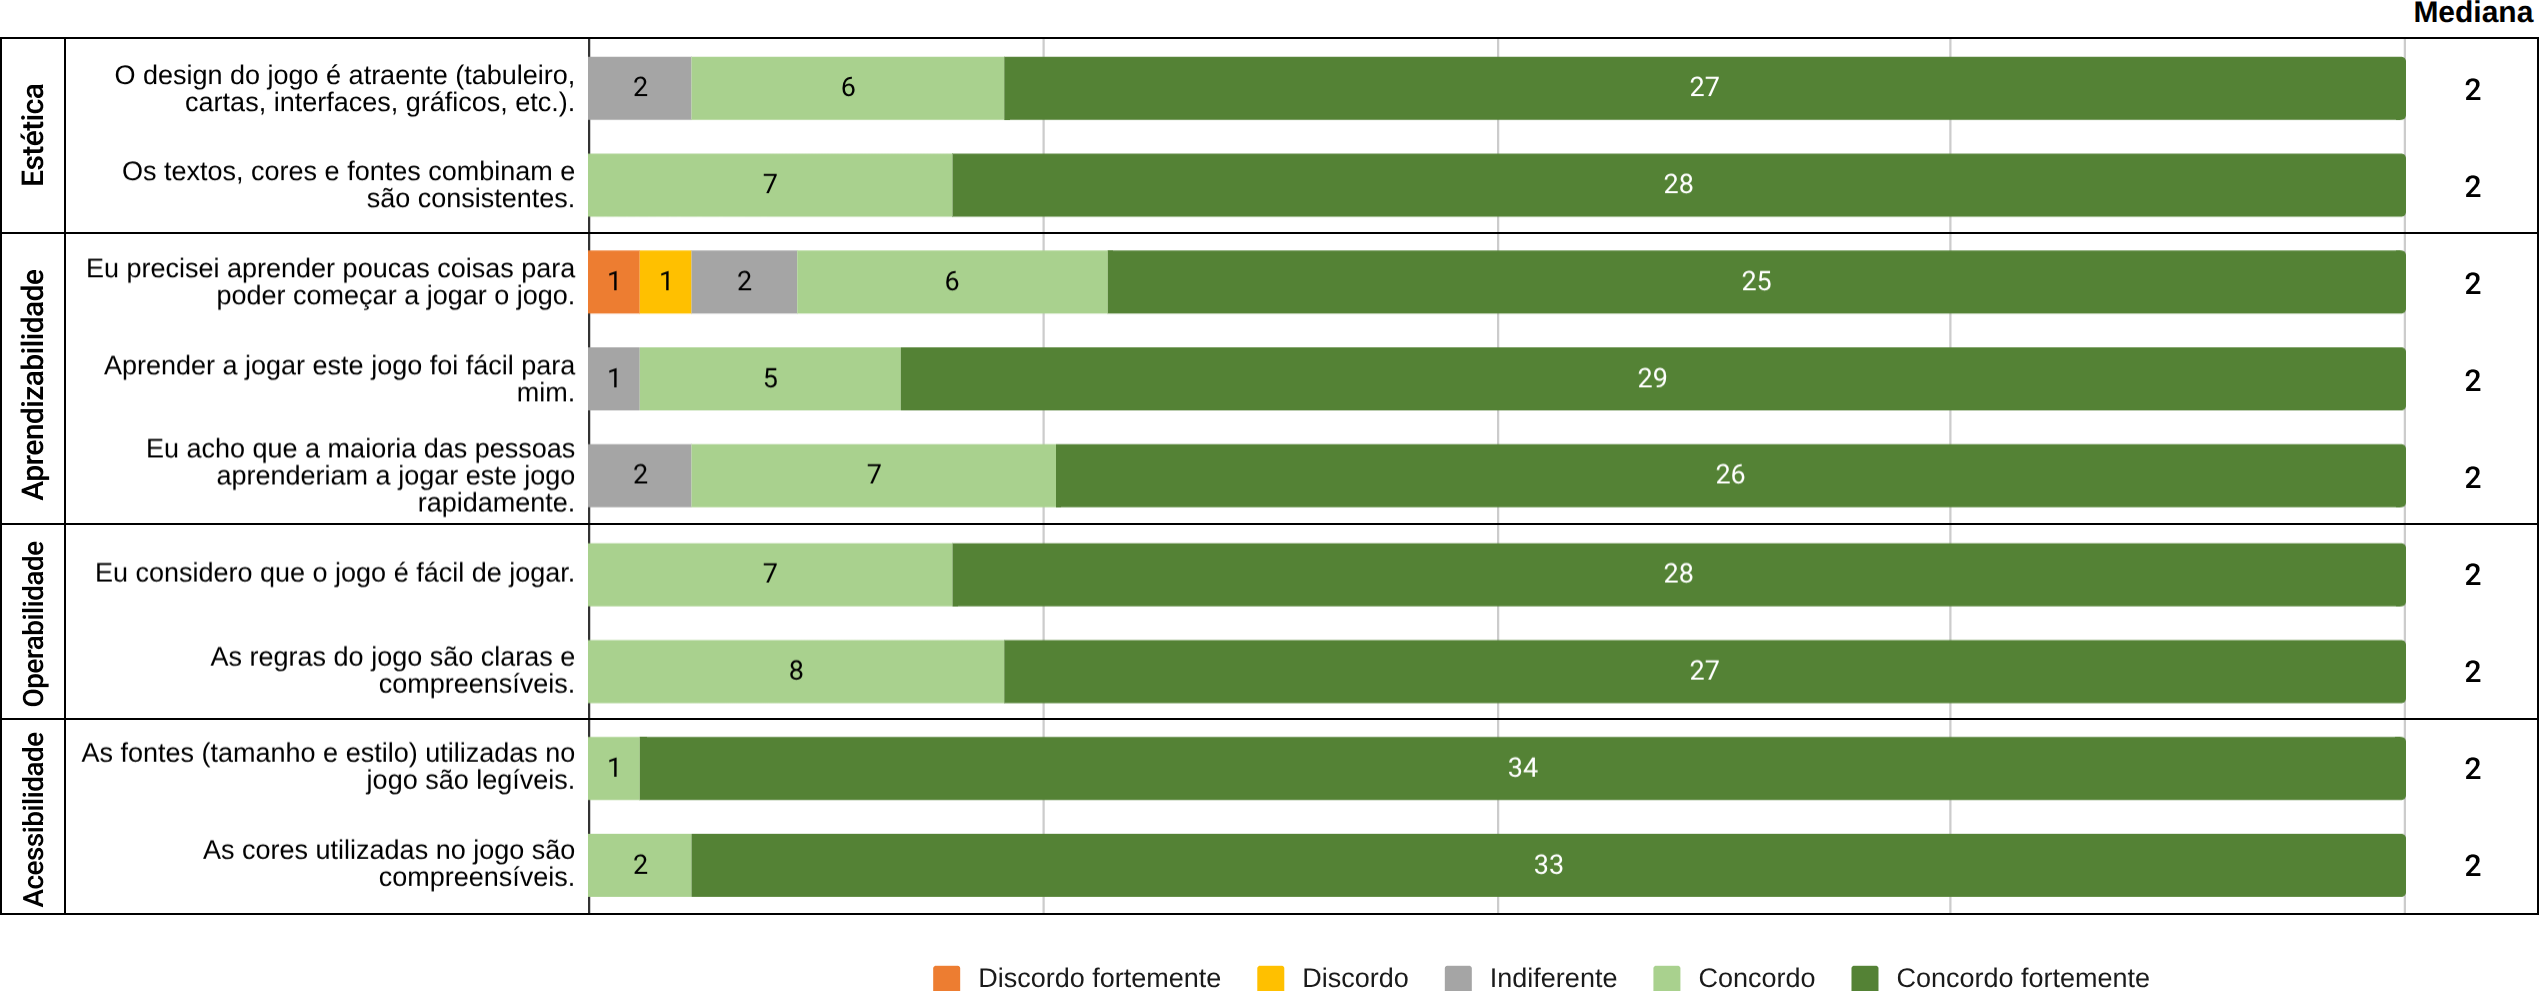
\includegraphics[width=\textwidth]{bridge-usabilidade}
	\legend{Fonte: Autora (2025)}
\end{figure}

No critério Experiência do Jogador, a Figura \ref{bridge-xp-jogador} ilustra os resultados obtidos. Um dos aspectos cruciais para a adoção de novas ferramentas é a facilidade de aprendizado. A análise revelou que itens como curva de aprendizado, clareza das regras e facilidade de jogar apresentaram mediana 2 (Concordo fortemente). A distribuição das respostas para esses itens mostrou uma grande maioria de votos entre 1 (Concordo) e 2 (Concordo fortemente), com pouquíssimas notas negativas. Este é um item fundamental, pois demonstra que a dinâmica é intuitiva e acessível, com um tempo de adaptação mínimo, o que é essencial para sua aplicação em grupos diversos e em contextos profissionais onde a otimização do tempo é prioritária. A eficácia da instrução e da estrutura da dinâmica é, portanto, um ponto forte.

Observa-se que a dinâmica demonstrou resultados positivos em diversos tópicos, mas especificamente nos itens relacionados a desafio adequado, tarefas não monótonas, sentimento de realização e satisfação com o aprendizado, a mediana foi 1 (Concordo). A distribuição das respostas para esses itens foi mais variada, apresentando uma maior dispersão, com alguns votos em 0 (Indiferente), -1 (Discordo) e até -2 (Discordo fortemente). Isso sugere que, embora a dinâmica seja percebida como fácil e clara, há oportunidades para torná-la mais desafiadora ou menos repetitiva, a fim de gerar um engajamento mais profundo e uma sensação de conquista mais pronunciada. Este é um espaço para a evolução de mecânicas ou a introdução de variações nas atividades que possam enriquecer a experiência a longo prazo.

A dimensão de interação social é crucial para dinâmicas em grupo. Os itens analisados, como interação com outras pessoas, cooperação/competição e sentimento durante a interação, obtiveram mediana 2, com uma alta concentração nas notas mais altas. Esse resultado indica que a dimensão social da dinâmica está funcionando muito bem, promovendo um ambiente colaborativo e positivo. Os jogadores se sentiram conectados e engajados com os outros participantes, o que é um ponto forte para fortalecer a cultura colaborativa e a comunicação dentro das equipes.

Para a análise dos itens diversão, momentos de alegria, atenção inicial e relevância do conteúdo revelou que todos obtiveram mediana 2 (Concordo fortemente). Houve pouquíssimos votos abaixo de 1 (Concordo). Isso demonstra que a dinâmica gera um engajamento emocional positivo desde o início e consegue manter o interesse dos participantes. Este é um fator fundamental para criar uma boa experiência e com maior retenção do aprendizado, pois a relevância do conteúdo é percebida de forma lúdica.

\begin{figure}[H]
	\caption{\label{bridge-xp-jogador} Resultados da avaliação de experiência do jogador com profissionais}
  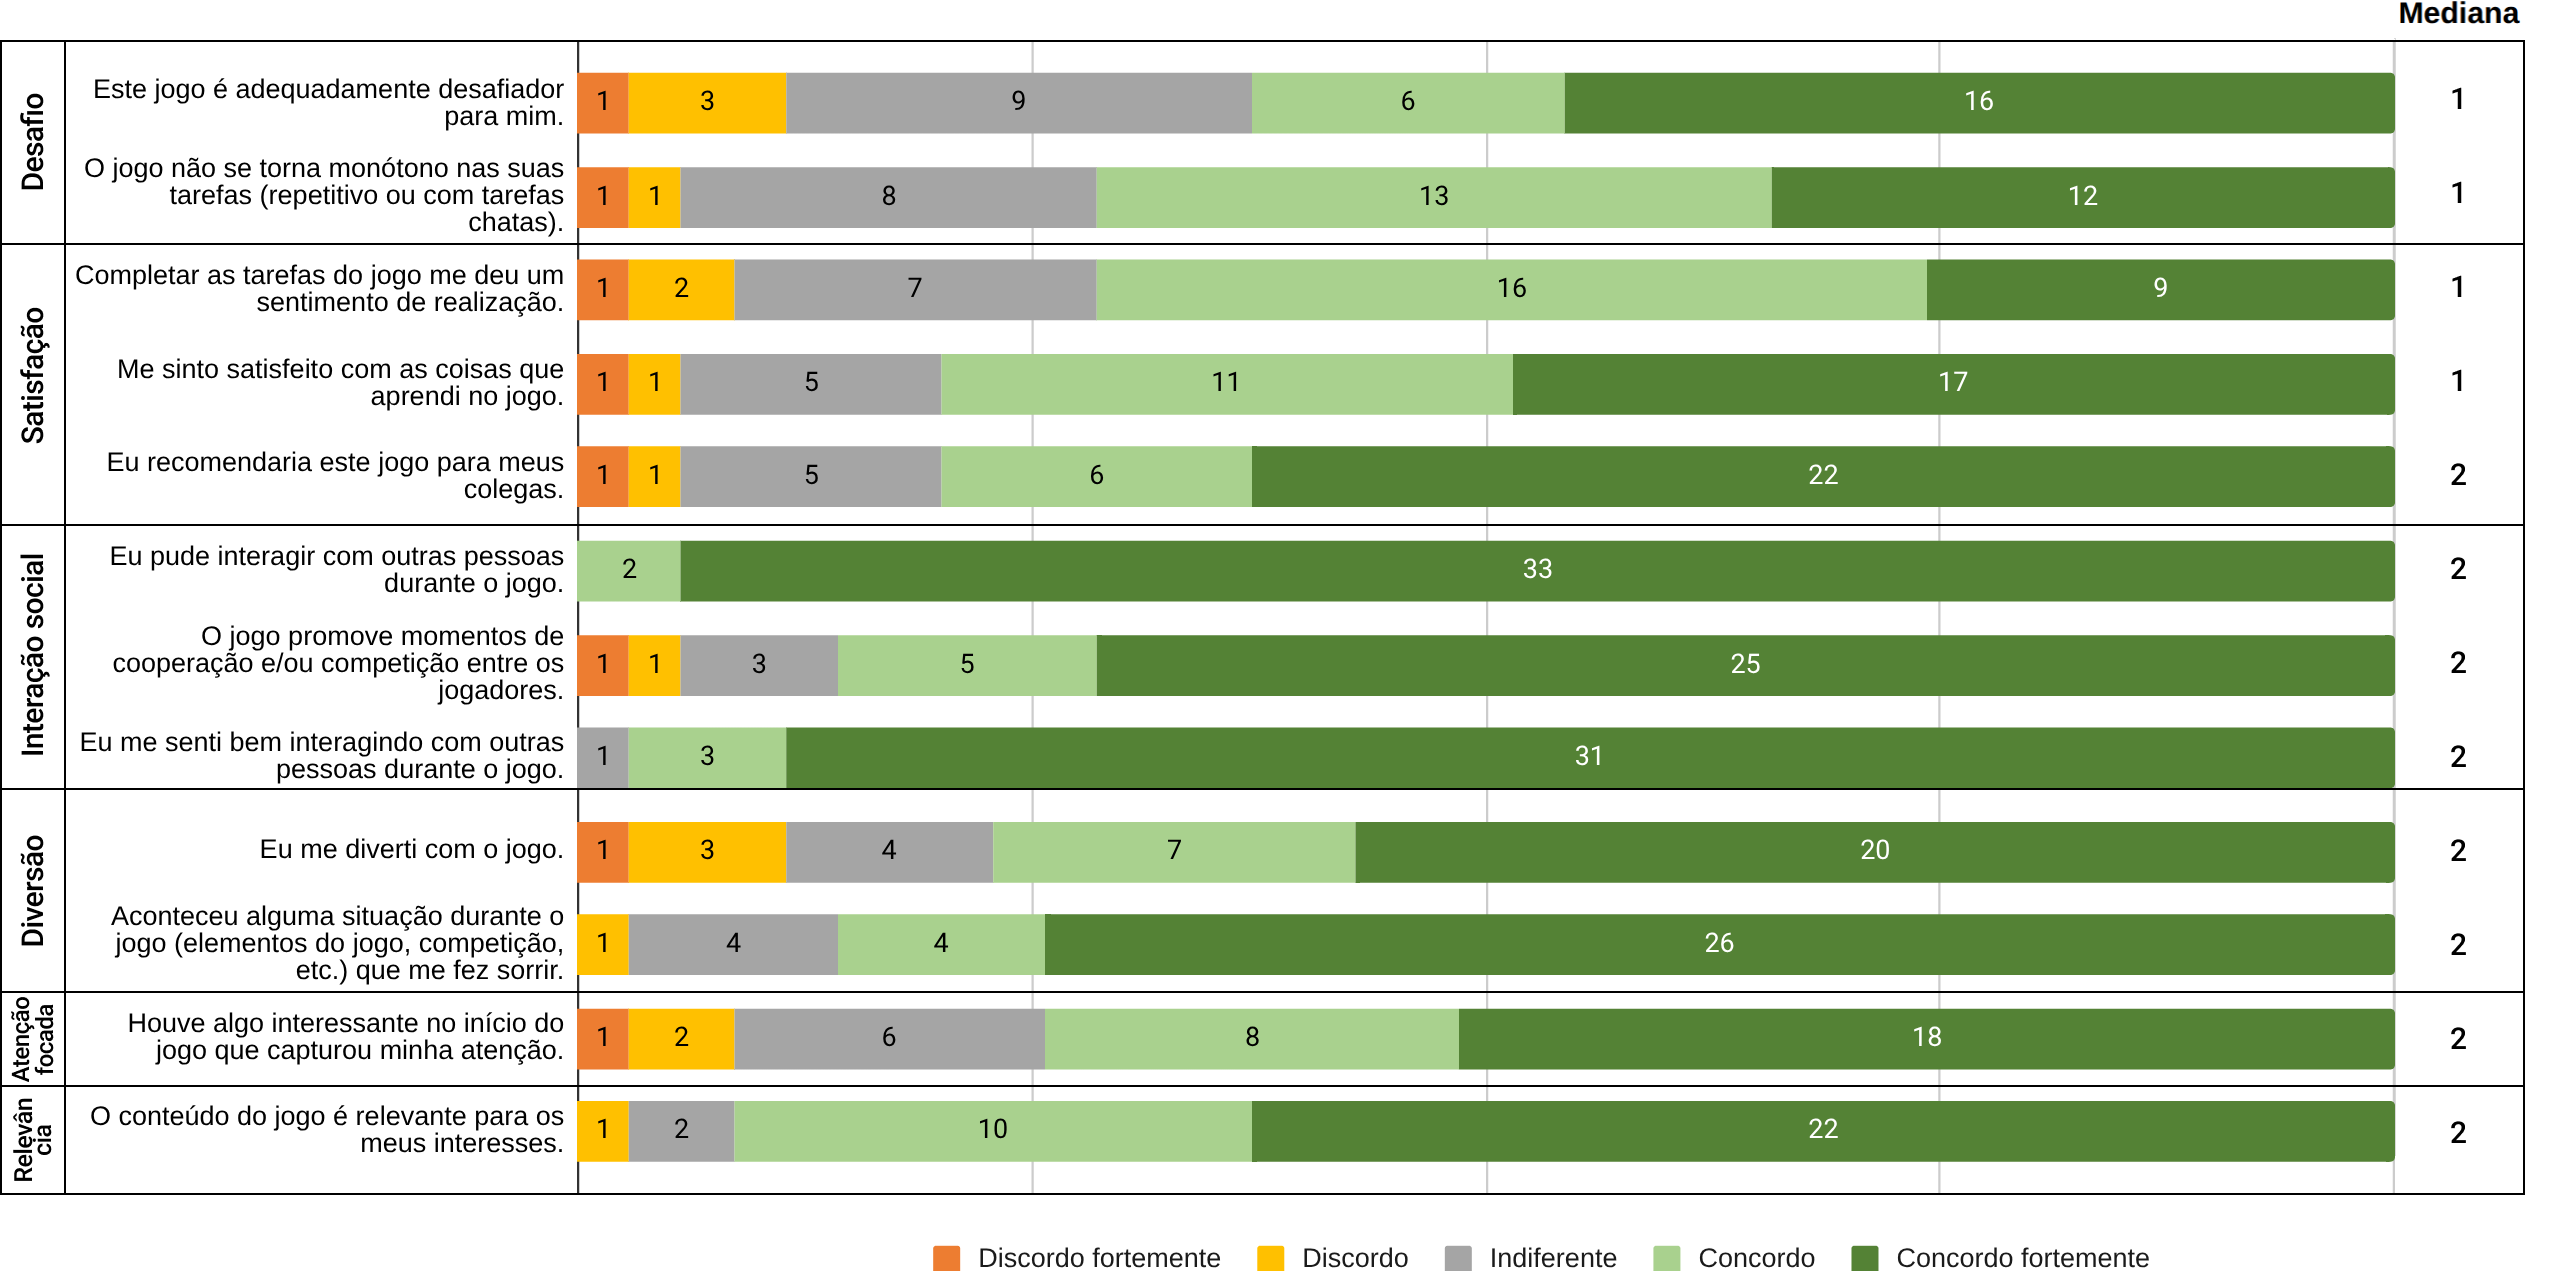
\includegraphics[width=\textwidth]{bridge-xp-jogador}
	\legend{Fonte: Autora (2025)}
\end{figure}

Considerando os objetivos gerais diretamente relacionados à identificação e análise de riscos, os itens analisados como percepção de riscos, vulnerabilidades e análise de riscos obtiveram mediana 2 (Concordo fortemente). A maioria dos votos concentrou-se entre 1 (Concordo) e 2 (Concordo fortemente). Este resultado, apresentado também na Figura \ref{bridge-afirmativas}, é crucial, pois confirma que a dinâmica cumpre eficazmente sua função. Os profissionais percebem que fizeram algo útil e diretamente aplicável ao contexto de seus projetos, validando a eficácia da ferramenta no atingimento de seus propósitos centrais.

\begin{figure}[H]
	\caption{\label{bridge-afirmativas} Resultados da avaliação de afirmativas específicas com profissionais}
  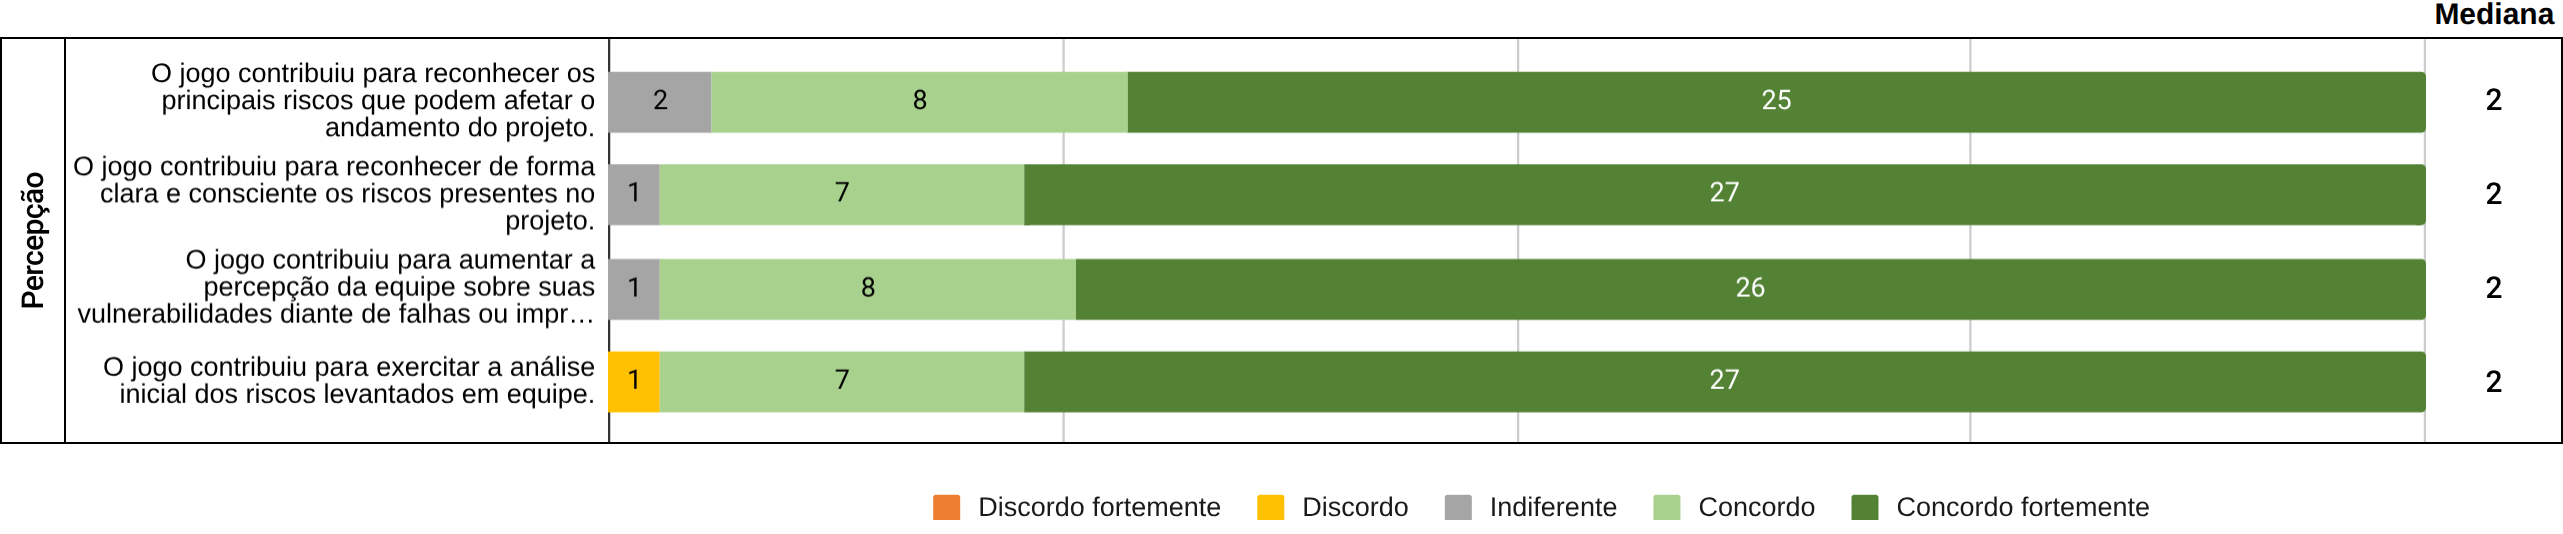
\includegraphics[width=\textwidth]{bridge-afirmativas}
	\legend{Fonte: Autora (2025)}
\end{figure}

Além dos dados quantitativos, o \textit{feedback} qualitativo dos profissionais revelou pontos de destaque e oportunidades de aprimoramento.

Os aspectos mais elogiados pelos participantes foram:
\begin{itemize}
  \item \textbf{Eficácia na identificação e análise de riscos}: Muitos profissionais destacaram a capacidade da dinâmica de levantar riscos que não haviam sido previamente definidos ou formalmente discutidos pela equipe. A ferramenta foi vista como um catalisador para debates e análises conjuntas, contribuindo para uma reflexão sobre vulnerabilidades e para a priorização de riscos importantes.
  \item \textbf{Formato lúdico e engajador}: A abordagem gamificada, com o design atrativo das cartas, personagens (como os  “pokemons” e seus nomes) e o sistema de moedas, foi amplamente elogiada por tornar a discussão de riscos mais descontraída, divertida, dinâmica e engajadora, mesmo em temas complexos. A facilidade de jogar e a interatividade foram pontos frequentemente mencionados.
  \item \textbf{Estímulo à interação e colaboração}: A dinâmica foi reconhecida por promover a participação ativa de todos os integrantes da equipe e por facilitar a integração e o debate saudável, o que, em muitos casos, resultou na primeira oportunidade formal de discutir riscos em conjunto.
  \item \textbf{Organização e clareza}: A objetividade dos textos das cartas e a clareza das perguntas foram destacadas por facilitar a identificação dos riscos. A organização visual do material também foi mencionada como um facilitador.
\end{itemize}

Quanto aos aspectos que poderiam ser aprimorados, as sugestões dos profissionais incluíram:
\begin{itemize}
  \item \textbf{Duração e fadiga}: Para o deck completo, alguns participantes relataram um certo cansaço ou queda na atenção ao longo da dinâmica, sugerindo que uma duração ideal poderia ser em torno de 1 hora.
  \item \textbf{Repetitividade e sobreposição de cartas}: Similar ao \textit{feedback} dos estudantes, houve menção a algumas cartas que pareciam ter temas muito parecidos ou elementos difíceis de diferenciar (ex:  “Stakeon” e  “Clientor”). A sugestão é revisar os textos ou o número de cartas para evitar redundâncias.
  \item \textbf{Clareza e formatação das perguntas}: Algumas sugestões pontuais sobre a redação das perguntas nas cartas foram feitas, indicando que a frase poderia estar diretamente formatada como um “risco” em vez de uma pergunta, para evitar ambiguidades na interpretação da concordância.
  \item \textbf{Ferramenta digital e usabilidade da plataforma}: Embora a aplicação remota tenha sido funcional, houve sugestões para aprimorar a experiência em plataformas digitais (ex: Figma), como o bloqueio de elementos de fundo e a consideração de um aplicativo interativo próprio, para evitar dificuldades técnicas.
  \item \textbf{Aprofundamento pós-dinâmica}: Alguns participantes apontaram a necessidade de uma sequência para a dinâmica, como um módulo ou ferramenta para organizar os planos de ação após o levantamento dos riscos.
  \item \textbf{Detalhes e explicabilidade}: Sugeriu-se que o manual ou as explicações poderiam ser ainda mais detalhadas, com exemplos ou vídeos práticos de uma rodada, para facilitar o entendimento inicial, especialmente sobre como considerar e registrar os riscos.
\end{itemize}

Essas percepções qualitativas dos profissionais são cruciais, pois complementam os dados quantitativos, oferecendo insights práticos e contextuais para futuras iterações e aprimoramentos da dinâmica.

\section{Discussão}
\label{sec:discussao}

Este capítulo apresentou a avaliação da dinâmica proposta, realizada em dois contextos distintos: com estudantes de graduação e com profissionais atuantes no mercado. A análise comparativa dos resultados quantitativos, obtidos por meio do questionário MEEGA+ adaptado, e das percepções qualitativas coletadas de ambos os públicos, permite uma compreensão aprofundada da eficácia, usabilidade e aplicabilidade da dinâmica.

Apesar da natureza distinta dos públicos e ambientes de aplicação, a dinâmica demonstrou consistentemente pontos fortes em diversas dimensões. Conforme observado tanto nas avaliações com estudantes quanto com profissionais, o design visual da dinâmica foi universalmente bem avaliado, com todos os itens atingindo mediana 2 (Concordo fortemente) em ambos os grupos. Essa unanimidade reforça que a qualidade estética e a clareza da apresentação são diferenciais importantes e contribuem positivamente para a experiência inicial do usuário.

Similarmente, a interação social foi um ponto de excelência em ambas as avaliações, com todos os itens sociais (interação, cooperação/competição e sentimentos positivos ao interagir) obtendo mediana 2 (Concordo fortemente). Isso evidencia a capacidade inerente da dinâmica em promover a colaboração e o engajamento entre os participantes, independentemente do seu nível de experiência ou contexto, o que é fundamental para atividades de análise de riscos em equipes ágeis.

Adicionalmente, os objetivos específicos da dinâmica foram consistentemente bem avaliados, com todas as afirmativas pertinentes a esses critérios atingindo mediana 2 (Concordo fortemente) em ambos os públicos. Isso inclui a clareza da relação com a disciplina/contexto, a aprendizagem proporcionada, a relevância do conteúdo e a contribuição direta para o reconhecimento e análise de riscos. Tal resultado confirma que a dinâmica cumpre com excelência sua função central de auxiliar na identificação e discussão de riscos, e é percebida como uma ferramenta didática e prática eficaz.

A comparação entre os dois grupos revelou discrepâncias em dimensões específicas, que fornecem insights para o aprimoramento da dinâmica e sua adequação a diferentes contextos de aplicação. As principais discrepâncias observadas são:

\begin{itemize}
  \item \textbf{Facilidade de aprendizado:} Os estudantes indicaram uma dificuldade significativamente maior para aprender a jogar e compreender as regras, em contraste com a percepção dos profissionais. A afirmativa “Eu precisei aprender poucas coisas para começar a jogar o jogo”, por exemplo, teve mediana 0 (Indiferente) para estudantes, enquanto para profissionais foi 2 (Concordo fortemente). Similarmente, outras afirmativas como “Aprender a jogar este jogo foi fácil para mim”, “Eu acho que a maioria das pessoas aprenderiam a jogar este jogo rapidamente”, “Eu considero que o jogo é fácil de jogar” e “As regras do jogo são claras e compreensíveis” apresentaram mediana 1 (Concordo) para estudantes e 2 (Concordo fortemente) para profissionais. Essa discrepância pode estar relacionada ao tempo limitado para a aplicação em sala de aula, à pressão inerente a um contexto acadêmico ou a uma menor familiaridade com o formato de gamificação para fins práticos. Isso sugere a necessidade de desenvolver um processo de onboarding mais robusto e contextualizado para ambientes educacionais, talvez com a inclusão de um vídeo instrutivo ou de uma rodada de exemplo.

  \item \textbf{Engajamento emocional e diversão:} Itens relacionados à diversão e ao sentimento de realização foram avaliados com medianas mais altas pelos profissionais. Afirmativas como “Me diverti com o jogo” e “Aconteceu algo no jogo que me fez sorrir” tiveram mediana 1 (Concordo) para estudantes e 2 (Concordo fortemente) para profissionais. O mesmo padrão foi observado para “O jogo não se torna monótono nas suas tarefas” e “Completar as tarefas do jogo me deu um sentimento de realização”, que também apresentaram mediana 1 (Concordo) para estudantes e 2 (Concordo fortemente) para profissionais. Além disso, a recomendação geral do jogo (”Eu recomendaria este jogo para meus colegas”) seguiu essa tendência, com mediana 1 (Concordo) para estudantes e 2 (Concordo fortemente) para profissionais. Isso indica que o aspecto lúdico e a sensação de conquista foram mais fortes fora da sala de aula. É provável que o ambiente mais formal da sala de aula tenha inibido o engajamento espontâneo e a expressividade emocional. Para otimizar o engajamento lúdico em contextos acadêmicos, seria benéfico criar um clima mais descontraído durante a aplicação e considerar a permissão de pausas para conversas livres, o que pode aumentar a imersão e o prazer na experiência.
\end{itemize}

Em síntese, a maior discrepância entre os dois públicos reside na percepção da facilidade de aprendizado e no nível de engajamento lúdico. A dinâmica demonstra um desempenho visual e pedagógico consistentemente elevado, validando sua concepção e seus objetivos centrais. Contudo, para que a experiência em sala de aula atinja o mesmo nível de fluidez e diversão percebido em ambientes profissionais, são necessários ajustes no processo de onboarding e na ambientação da atividade. A promoção de um ambiente mais descontraído para mitigar as diferenças observadas e maximizar o potencial da dinâmica em diferentes contextos de aplicação.

% TODO (esse negócio do onboarding tá meio repetitivo)

\section{Ameaças à validade}

A condução de qualquer estudo empírico, incluindo a avaliação de uma dinâmica de gamificação, está sujeita a diversas ameaças à validade que podem limitar a generalização e a confiança nos resultados obtidos. Esta seção discute as potenciais ameaças à validade identificadas neste estudo, categorizando-as de acordo com a taxonomia comum de validação de pesquisa, e propondo estratégias para mitigar seus impactos.

\subsection{Ameaças à validade de construto}
\label{sec:ameacas-construto}

A validade de construto refere-se à extensão em que as variáveis operacionais (como a forma de medir a usabilidade ou a diversão da dinâmica) realmente representam os construtos teóricos que se pretende medir.
\begin{itemize}
  \item \textbf{Subjetividade das percepções:} A principal ameaça aqui reside na natureza subjetiva das respostas aos questionários. A percepção de “diversão”, “facilidade de uso” ou “relevância” pode variar amplamente entre os participantes, influenciada por fatores pessoais, expectativas prévias ou até mesmo o humor no momento da avaliação.
  \begin{itemize}
    \item \textit{Mitigação:} A utilização de um modelo de avaliação consolidado como o MEEGA+ (mesmo que adaptado) ajuda a padronizar a coleta de dados, mas a interpretação ainda é individual. A combinação de dados quantitativos (questionário) com dados qualitativos (comentários abertos) foi utilizada para fornecer uma visão mais completa e triangulada das percepções.
    \end{itemize}
  \item \textbf{Interpretação das perguntas do questionário:} Embora o questionário tenha sido adaptado e revisado, sempre existe o risco de que os participantes interpretem as perguntas de maneira diferente do que foi intencionado pelos pesquisadores. Isso pode levar a respostas que não refletem precisamente o construto que se desejava medir.
  \begin{itemize}
    \item \textit{Mitigação:} A clareza na redação das perguntas e a oportunidade para os participantes tirarem dúvidas durante as aplicações (especialmente na modalidade presencial) foram consideradas.
    \end{itemize}
  \item \textbf{Adaptação do instrumento de avaliação:} A adaptação de um instrumento de avaliação consolidado, como o corte de itens do MEEGA+ \cite{MEEGA}, representa uma ameaça potencial à validade de construto. A modificação de um instrumento validado pode comprometer suas propriedades psicométricas originais, uma vez que a retirada de itens pode alterar o que o instrumento de fato mede. Consequentemente, não é possível assegurar que o instrumento adaptado mede precisamente os mesmos construtos que a versão original, impactando a validade dos resultados obtidos.
  \begin{itemize}
    \item \textit{Mitigação:} A adaptação foi realizada buscando manter a essência dos construtos originais relevantes para a avaliação de gamificação. A análise dos resultados das afirmativas específicas, que foram customizadas, visa complementar a visão obtida pelos itens gerais do MEEGA+ adaptado.
    \end{itemize}
  \item \textbf{Efeito Hawthorne:} A participação em um estudo pode, por si só, alterar o comportamento ou as respostas dos indivíduos. Os participantes podem ter se esforçado mais na dinâmica ou fornecido respostas mais positivas no questionário simplesmente por saberem que estavam sendo parte de uma avaliação.
  \begin{itemize}
    \item \textit{Mitigação:} A garantia de anonimato nas respostas do questionário pode reduzir esse efeito, mas não eliminá-lo completamente. A aplicação por \textit{Scrum Masters}, sem a presença constante da autora, também pode ter ajudado a reduzir a percepção de uma avaliação direta.
    \end{itemize}
\end{itemize}

\subsection{Ameaças à validade interna}
\label{sec:ameacas-interna}

A validade interna preocupa-se com a extensão em que a relação de causa e efeito observada entre as variáveis é realmente genuína e não influenciada por fatores externos ou confounding factors.

\begin{itemize}
  \item \textbf{Diferenças entre grupos de aplicação:} As características dos grupos (estudantes vs. profissionais, número de participantes por grupo, decks de cartas utilizados, tempo de aplicação) variaram. Essas diferenças podem ter influenciado os resultados e as percepções dos participantes, em vez de serem causadas exclusivamente pela dinâmica em si.
  \begin{itemize}
    \item \textit{Mitigação:} A análise separada dos resultados para cada grupo e a identificação das discrepâncias (como feito na seção de discussão) buscam contextualizar essas variações. No entanto, a impossibilidade de randomizar completamente as condições de aplicação é uma limitação inerente.
    \end{itemize}
  \item \textbf{Envolvimento e potencial viés da pesquisadora:} A presença e influência da pesquisadora nos momentos de avaliação podem representar uma ameaça. Como a autora esteve envolvida de maneira próxima e ativa no processo de coleta de dados e avaliação, especialmente na aplicação com sua própria equipe, pode ter ocorrido uma influência inadvertida nos resultados. A pesquisadora pode, mesmo que inconscientemente, introduzir seus próprios preconceitos, expectativas ou interpretações nos dados coletados, comprometendo a objetividade e a validade interna do estudo. Para uma validação mais robusta desses resultados, seria necessária uma avaliação prática sem a participação ativa da autora, por um terceiro imparcial.
  \begin{itemize}
    \item \textit{Mitigação:} Como contorno desta limitação, a autora buscou manter uma postura neutra e imparcial durante as aplicações, abstendo-se de influenciar as discussões ou respostas dos participantes. Além disso, a maioria das aplicações com profissionais foi conduzida pelos próprios \textit{Scrum Masters} das equipes, o que reduziu a presença direta da autora.
    \end{itemize}
  \item \textbf{Maturação:} O conhecimento prévio dos participantes sobre gestão de riscos ou sobre gamificação pode ter evoluído durante o período do estudo, influenciando suas respostas.
    \begin{itemize}
    \item \textit{Mitigação:} As aplicações foram relativamente curtas, o que minimiza o efeito da maturação em termos de aquisição de novos conhecimentos significativos durante a dinâmica.
    \end{itemize}
  \item \textbf{História:} Eventos externos que ocorreram durante o período das aplicações (e.g., projetos em crise, pressão de prazos) podem ter afetado o humor, a atenção e a percepção dos participantes sobre a dinâmica.
    \begin{itemize}
    \item \textit{Mitigação:} É difícil controlar todos os eventos externos na vida dos participantes. A aplicação em múltiplos grupos em momentos distintos pode diluir o impacto de um evento isolado em um único grupo.
    \end{itemize}
\end{itemize}

\subsection{Ameaças à validade externa}
\label{sec:ameacas-externa}

A validade externa refere-se à capacidade de generalizar os resultados do estudo para outras populações, ambientes ou contextos fora do escopo da pesquisa.

\begin{itemize}
  \item \textbf{Estratégia de seleção da amostra e viés de seleção:} A estratégia de seleção da amostra adotada, caracterizada por ser de conveniência e, em parte, por vínculos pessoais com os profissionais envolvidos no Laboratório Bridge, pode introduzir um viés de seleção. Essas conexões pré-existentes podem ter influenciado a escolha dos participantes, resultando em uma amostra que pode não ser totalmente representativa de uma população mais ampla de profissionais ou estudantes. Essa limitação compromete a generalização dos resultados e, consequentemente, a validade externa do estudo.
    \begin{itemize}
    \item \textit{Mitigação:} Embora inerente a estudos com amostras de conveniência, a avaliação em dois públicos distintos (acadêmicos e profissionais) e com diferentes níveis de experiência tenta expandir um pouco a representatividade dos resultados. A descrição do perfil dos participantes busca fornecer transparência sobre as características da amostra.
    \end{itemize}
  \item \textbf{Contexto específico da aplicação:} A dinâmica foi aplicada em um ambiente de sala de aula e em um laboratório de pesquisa e desenvolvimento. As características desses ambientes (e.g., cultura da equipe, tipo de projeto, familiaridade com ferramentas ágeis) podem não ser representativas de todos os cenários de desenvolvimento de \textit{software}.
    \begin{itemize}
    \item \textit{Mitigação:} A documentação do contexto de aplicação busca fornecer subsídios para que futuros pesquisadores possam avaliar a similaridade com seus próprios ambientes.
    \end{itemize}
  \item \textbf{Modalidade de aplicação (remota/FigJam):} A maioria das aplicações com profissionais foi em ambiente remoto, utilizando ferramentas como o FigJam. Isso pode ter influenciado a interação e a percepção da dinâmica em comparação com uma aplicação presencial com materiais físicos.
    \begin{itemize}
    \item \textit{Mitigação:} A identificação clara da modalidade de aplicação permite que o leitor pondere os resultados sob essa luz. A comparação com a aplicação presencial com alunos (onde a dinâmica é física) pode fornecer alguns insights, embora não seja uma comparação direta devido às outras variáveis.
    \end{itemize}
\end{itemize}

\subsection{Ameaças à validade de conclusão estatística}
\label{sec:ameacas-estatistica}

Esta validade diz respeito à inferência correta da relação entre as variáveis utilizando métodos estatísticos.

\begin{itemize}
  \item \textbf{Tamanho da amostra:} O número total de participantes (45 estudantes e 43 profissionais) e o número de respostas ao questionário (30 e 35, respectivamente) podem ser considerados moderados para algumas análises estatísticas mais robustas, limitando o poder de detectar efeitos pequenos, mas relevantes.
    \begin{itemize}
    \item \textit{Mitigação:} A análise baseou-se principalmente em medianas e frequências percentuais, que são adequadas para tamanhos de amostra menores e dados ordinais (escala Likert). A complementação com dados qualitativos também fortalece a interpretação dos resultados.
    \end{itemize}
  \item \textbf{Variabilidade dentro dos grupos:} As variações nas condições de aplicação entre as equipes de profissionais (sub-decks diferentes, tempos variados, foco abrangente vs. específico) podem ter aumentado a variabilidade dos dados, dificultando a identificação de padrões claros.
    \begin{itemize}
    \item \textit{Mitigação:} A descrição dessas variações na seção da avaliação com os profissionais ajuda a contextualizar os resultados. Em futuras pesquisas, uma maior padronização das condições de aplicação seria ideal para reduzir essa variabilidade.
    \end{itemize}
\end{itemize}

%------------------------------------------------------------------------------%
%------------------------------------------------------------------------------%

\chapter{Conclusão}
\label{cap:conclusao}

O presente trabalho teve como objetivo principal desenvolver e avaliar uma dinâmica gamificada para auxiliar na análise e identificação de riscos em equipes ágeis de desenvolvimento de \textit{software}. Para alcançar este propósito, o estudo foi estruturado em uma série de etapas metodológicas que permitiram a construção de uma base teórica sólida, o entendimento do estado da arte na gestão de riscos em contextos ágeis, o desenvolvimento da dinâmica e sua posterior avaliação em diferentes ambientes e com distintos públicos.

Inicialmente, a pesquisa realizou uma análise e fundamentação teórica abrangente, abordando conceitos essenciais de gerência de projetos, gestão de riscos, métodos ágeis e gamificação. Este embasamento conceitual, detalhado no Capítulo \ref{cap:fundamentacao-teorica}, foi crucial para contextualizar a problemática e guiar as etapas subsequentes do trabalho. Complementarmente, um mapeamento sistemático da literatura, apresentado no Capítulo \ref{cap:estado-arte}, foi conduzido com o intuito de identificar e analisar os riscos mais comuns em projetos ágeis, as técnicas de gestão de riscos prevalentemente utilizadas e os resultados obtidos com a aplicação de tais práticas. Esse levantamento do estado da arte forneceu insights valiosos que fundamentaram a concepção e o desenvolvimento da dinâmica gamificada.

A partir da revisão teórica e do mapeamento sistemático, foi identificada a necessidade de uma ferramenta mais interativa e engajadora para facilitar a gestão de riscos, especialmente a etapa de identificação e análise. Com base nessa lacuna, o desenvolvimento da dinâmica gamificada foi realizado, seguindo uma abordagem estruturada que incluiu a definição de objetivos, análise do público-alvo e prototipagem da solução, conforme detalhado no Capítulo \ref{cap:proposta} e \ref{cap:dinamica-execucao}. O material resultante, composto por cartas de riscos e um guia de aplicação, foi projetado para ser intuitivo e adaptável.

A avaliação da dinâmica foi um pilar central deste trabalho, visando analisar a motivação, experiência do usuário e aprendizagem proporcionada pela proposta gamificada. Conforme apresentado no Capítulo \ref{cap:avaliacao}, a dinâmica foi aplicada com dois públicos distintos: estudantes de graduação da Universidade Federal de Santa Catarina (UFSC) e profissionais do mercado de trabalho, em contextos de projetos ágeis reais. Os resultados dessa avaliação foram predominantemente positivos em diversas dimensões.

As avaliações com ambos os públicos, conforme discutido na seção \ref{sec:discussao}, evidenciaram que a dinâmica se destaca em aspectos cruciais. O design visual e a apresentação estética do material foram unanimemente elogiados, contribuindo para uma experiência agradável e profissional. A dimensão de interação social também obteve alta aprovação, confirmando a eficácia da dinâmica em promover a colaboração e o engajamento entre os participantes. Mais importante, os objetivos pedagógicos e a conexão com o conteúdo sobre riscos foram amplamente reconhecidos, indicando que a dinâmica cumpre sua função de auxiliar na identificação e análise de riscos de forma clara e relevante, sendo até preferível a outros métodos tradicionais por alguns participantes.

Contudo, a comparação entre os grupos de estudantes e profissionais revelou discrepâncias notáveis. A facilidade de aprendizado e o engajamento emocional/diversão foram percebidos de forma mais acentuada pelos profissionais. As medianas mais baixas e a maior dispersão de respostas entre os estudantes sugerem que o ambiente acadêmico, com suas limitações de tempo e potencial pressão avaliativa, pode ter inibido parte do aspecto lúdico e intuitivo da dinâmica, demandando um processo adaptado mais direcionado e uma ambientação mais descontraída para esse público.

Em síntese, este trabalho demonstra que a dinâmica gamificada desenvolvida é uma abordagem promissora e eficaz para a análise e identificação de riscos em equipes ágeis. Ela se mostrou capaz de engajar os participantes de forma interativa, promover a colaboração e, de maneira mais significativa, facilitar a compreensão e o reconhecimento de riscos em projetos de \textit{software}.

\section{Trabalhos futuros}
\label{sec:trabalhos-futuros}

Como indicação para trabalhos futuros, sugere-se a expansão e o aprimoramento da dinâmica em diversas frentes:

\begin{itemize}
\item \textbf{Expansão do conteúdo das cartas:} A criação de cartas para os demais riscos identificados na taxonomia usada como base \cite{Taxonomy} (32 elementos menos citados na literatura ficaram de fora da dinâmica) pode enriquecer ainda mais a dinâmica, tornando-a mais abrangente e útil para equipes que enfrentam uma variedade maior de desafios em projetos de \textit{software}.
\item \textbf{Aplicação em outros contextos:} É recomendada a aplicação da dinâmica em outros contextos além dos investigados neste estudo, como em projetos de \textit{software} não ágeis ou em empresas de diferentes portes e segmentos. Tal expansão pode ampliar a aplicabilidade da abordagem e validar sua eficácia em cenários mais diversificados.
\item \textbf{Aprofundamento pós-dinâmica:} Um ponto de melhoria dos \textit{feedbacks} foi a necessidade de uma sequência para a dinâmica. Sugere-se o desenvolvimento de um módulo ou ferramenta complementar que auxilie as equipes a organizar e planejar planos de ação após o levantamento e análise inicial dos riscos, transformando o input da dinâmica em saídas acionáveis para o projeto.
\item \textbf{Desenvolvimento de plataforma online:} A criação de uma plataforma online para a dinâmica representaria um avanço significativo, permitindo que equipes distribuídas participem da atividade de forma assíncrona ou síncrona de maneira mais facilitada. Isso ampliaria o alcance e a flexibilidade da abordagem, oferecendo uma experiência mais dinâmica e interativa para ambientes remotos ou híbridos.
\end{itemize}

%------------------------------------------------------------------------------%


% Referências -----------------------------------------------------------------%

\postextual
\bibliography{tcc}

% Apêndices -----------------------------------------------------------------%

\cleardoublepage
\phantomsection 
\addcontentsline{toc}{chapter}{APÊNDICES}
\thispagestyle{empty}
\vspace*{\fill}
\begin{center}
    \textbf{\Huge APÊNDICES}
\end{center}
\vspace*{\fill}
%\cleardoublepage

\begin{apendices}

\chapter{Strings de busca adaptadas}\label{apendiceA}

\vspace{-2em} % Ajusta o espaço negativo para reduzir a distância 

\begin{table}[h!]
  \centering
  \begin{tabular}{|l|p{12cm}|}
    \hline
    \textbf{Biblioteca digital} & \textbf{String adaptada} \\
    \hline
    ACM & (Title:(risk) OR Abstract:(risk)) AND (Title:(agile) OR Title:(scrum) OR Title:(xp) OR Title:(extreme programming) OR Title:(lean) OR Title:(kanban) OR Title:(scrumban) OR Title:(fdd) OR Title:(feature driven development) OR Title:(crystal) OR Title:(iterative development) OR Abstract:(agile) OR Abstract:(scrum) OR Abstract:(xp) OR Abstract:(extreme programming) OR Abstract:(lean) OR Abstract:(kanban) OR Abstract:(scrumban) OR Abstract:(fdd) OR Abstract:(feature driven development) OR Abstract:(crystal) OR Abstract:(iterative development)) AND (Title:(software) OR Abstract:(software)) \\
    \hline
    IEEExplore & "All Metadata":risk AND ("All Metadata":agile OR "All Metadata":scrum OR "All Metadata":xp OR "All Metadata":extreme programming OR "All Metadata":lean OR "All Metadata":kanban OR "All Metadata":scrumban OR "All Metadata":fdd OR "All Metadata":feature driven development OR "All Metadata":crystal OR "All Metadata":iterative development) AND "All Metadata":software \\
    \hline
    Scopus & (TITLE-ABS-KEY ( risk ) AND ( TITLE-ABS-KEY ( agile ) OR TITLE-ABS-KEY ( scrum ) OR TITLE-ABS-KEY ( xp ) OR TITLEABS-KEY ( extreme AND programming ) OR TITLE-ABS-KEY ( kanban ) OR TITLE-ABS-KEY ( scrumban ) OR TITLE-ABSKEY ( fdd ) OR TITLE-ABS-KEY ( feature AND driven AND development) OR TITLE-ABS-KEY ( crystal ) OR TITLE-ABS-KEY ( iterative AND development )) AND TITLE-ABS-KEY (software) AND ( LIMIT-TO ( SUBJAREA,"COMP") ) ) \\
    \hline
  \end{tabular}
\end{table}

\chapter{Estudos selecionados}
\label{apendiceB}

\vspace{-2em} % Ajusta o espaço negativo para reduzir a distância

\begin{longtable}{|c|p{5.5cm}|p{7.5cm}|}
  \hline
  \textbf{Estudo} & \textbf{Título} & \textbf{Referência} \\
  \hline
  \endfirsthead
  \hline
  \multicolumn{3}{|c|}{\textit{Continua na próxima página}} \\
  \hline
  \endfoot
  \hline
  \multicolumn{3}{|c|}{\textit{Fim da tabela}} \\
  \hline
  \endlastfoot
  S1 & RM3: A Risk Management Framework for IT Project Success & Paulo Roberto Martins de Andrade and Samira Sadaoui. 2021. RM3: A Risk Management Framework For IT Project Success. In Proceedings of the 4th International Conference on Computer Science and Software Engineering (CSSE '21). Association for Computing Machinery, New York, NY, USA, 200–205. \\
  \hline
  S2 & A novel risk management model in the Scrum and extreme programming hybrid methodology & Afshari, Mahnaz \& Javdani Gandomani, Taghi. (2022). A novel risk management model in the Scrum and extreme programming hybrid methodology. International Journal of Electrical and Computer Engineering. 12. 2911-2921. 10.11591/ijece.v12i3.pp2911-2921. \\
  \hline
  S3 & Risk management framework in Agile software development methodology & Zahedi, Mohammad \& Kashanaki, Alireza \& Farahani, Elham. (2023). Risk management framework in Agile software development methodology. International Journal of Electrical and Computer Engineering (IJECE). 13. 4379. 10.11591/ijece.v13i4.pp4379-4387. \\
  \hline
  S4 & SERGE – Serious Game for the Education of Risk Management in Software Project Management & G. Annunziata, S. Lambiase, F. Palomba and F. Ferrucci, “SERGE - Serious Game for the Education of Risk Management in Software Project Management,” 2024 IEEE/ACM 46th International Conference on Software Engineering: Software Engineering Education and Training (ICSE-SEET), Lisbon, Portugal, 2024, pp. 264-273, doi: 10.1145/3639474.3640085. \\
  \hline
  S5 & Do scaling agile frameworks address global software development risks? An empirical study & Beecham, Sarah \& Clear, Tony \& Lal, Ramesh \& Noll, John. (2021). Do scaling agile frameworks address global software development risks? An empirical study. Journal of Systems and Software. 171. 110823. 10.1016/j.jss.2020.110823. \\
  \hline
  S6 & User Story Risk Prioritization Model for Agile Software Development & P. Thanomwong and T. Senivongse, “User Story Risk Prioritization Model for Agile Software Development,” 2022 International Conference on Data and Software Engineering (ICoDSE), Denpasar, Indonesia, 2022, pp. 161-166, doi: 10.1109/ICoDSE56892.2022.9972041. \\
  \hline
  S7 & Issues of Formalization of Risk Management Process in Software Design & BILOUSIVA, Liudmyla et al. Issues of formalization of risk management process in software design. In: IntelITSIS. 2023. p. 48-57. \\
  \hline
\end{longtable}
\legend{Fonte: Autora (2024)}


\chapter{Riscos categorizados}
\label{apendiceC}

\vspace{-2em} % Ajusta o espaço negativo para reduzir a distância

%\renewcommand{\arraystretch}{1.2} 

\begin{longtable}{|>{\raggedright\arraybackslash}p{2.4cm}|p{4.5cm}|p{4.7cm}|l|}
  \hline
  \textbf{Classe} & \textbf{Elemento} & \textbf{Atributo} & \textbf{Estudo} \\
  \hline
  \endfirsthead
  \hline
  \multicolumn{4}{|c|}{\textit{Continua na próxima página}} \\
  \hline
  \endfoot
  \hline
  \multicolumn{4}{|c|}{\textit{Fim da tabela}} \\
  \hline
  \endlastfoot
  A. Product Engineering & 1. Requirements & a. Stability & S5, S6, S7 \\
  \cline{3-4}
  & & b. Completeness & S4, S6 \\
  \cline{3-4}
  & & c. Clarity & S4, S5, S6 \\
  \cline{3-4}
  & & d. Validity & S4, S5, S6 \\
  \cline{3-4}
  & & e. Feasibility & S4, S5, S6 \\
  \cline{3-4}
  & & g. Scale & S5 \\
  \cline{2-4}
  & 2. Design & b. Difficulty & S4 \\
  \cline{2-4}
  & 3. Code and Unit Test & a. Feasibility & S5 \\
  \cline{3-4}
  & & b. Testing & S7 \\
  \cline{2-4}
  & 5. Engineering Specialties & b. Reliability & S5 \\
  \hline
  B. Development Environment & 1. Development Process & c. Process Control & S5 \\
  \cline{3-4}
  & & d. Familiarity & S1, S5 \\
  \cline{2-4}
  & 2. Development System & a. Capacity & S5 \\
  \cline{3-4}
  & & d. Familiarity & S5 \\
  \cline{2-4}
  & 3. Management Process & a. Planning & S1, S5 \\
  \cline{3-4}
  & & c. Management Experience & S5 \\
  \cline{3-4}
  & & d. Program Interfaces & S1 \\
  \cline{2-4}
  & 4. Management Methods & a. Monitoring & S5 \\
  \cline{3-4}
  & & b. Personnel Management & S5 \\
  \cline{2-4}
  & 5. Work Environment & a. Quality Attitude & S1 \\
  \cline{3-4}
  & & b. Cooperation & S4, S5 \\
  \cline{3-4}
  & & c. Communication & S1, S4, S5 \\
  \cline{3-4}
  & & d. Morale & S5 \\
  \hline
  C. Program Constraints & 1. Resources & a. Schedule & S1, S4, S5, S7 \\
  \cline{3-4}
  & & b. Staff & S1, S5, S7 \\
  \cline{3-4}
  & & c. Budget & S4, S5 \\
  \cline{2-4}
  & 2. Contract & c. Dependencies & S5 \\
  \cline{2-4}
  & 3. Program Interfaces & a. Customer & S5, S7 \\
  \cline{3-4}
  & & b. Associate Contractors & S1, S5 \\
  \cline{3-4}
  & & e. Corporate Management & S5 \\
  \cline{3-4}
  & & f. Vendors & S5 \\
  \cline{3-4}
  & & g. Politics & S5 \\
  \hline
\end{longtable}

\chapter{Projeto fictício}
\label{apendiceD}

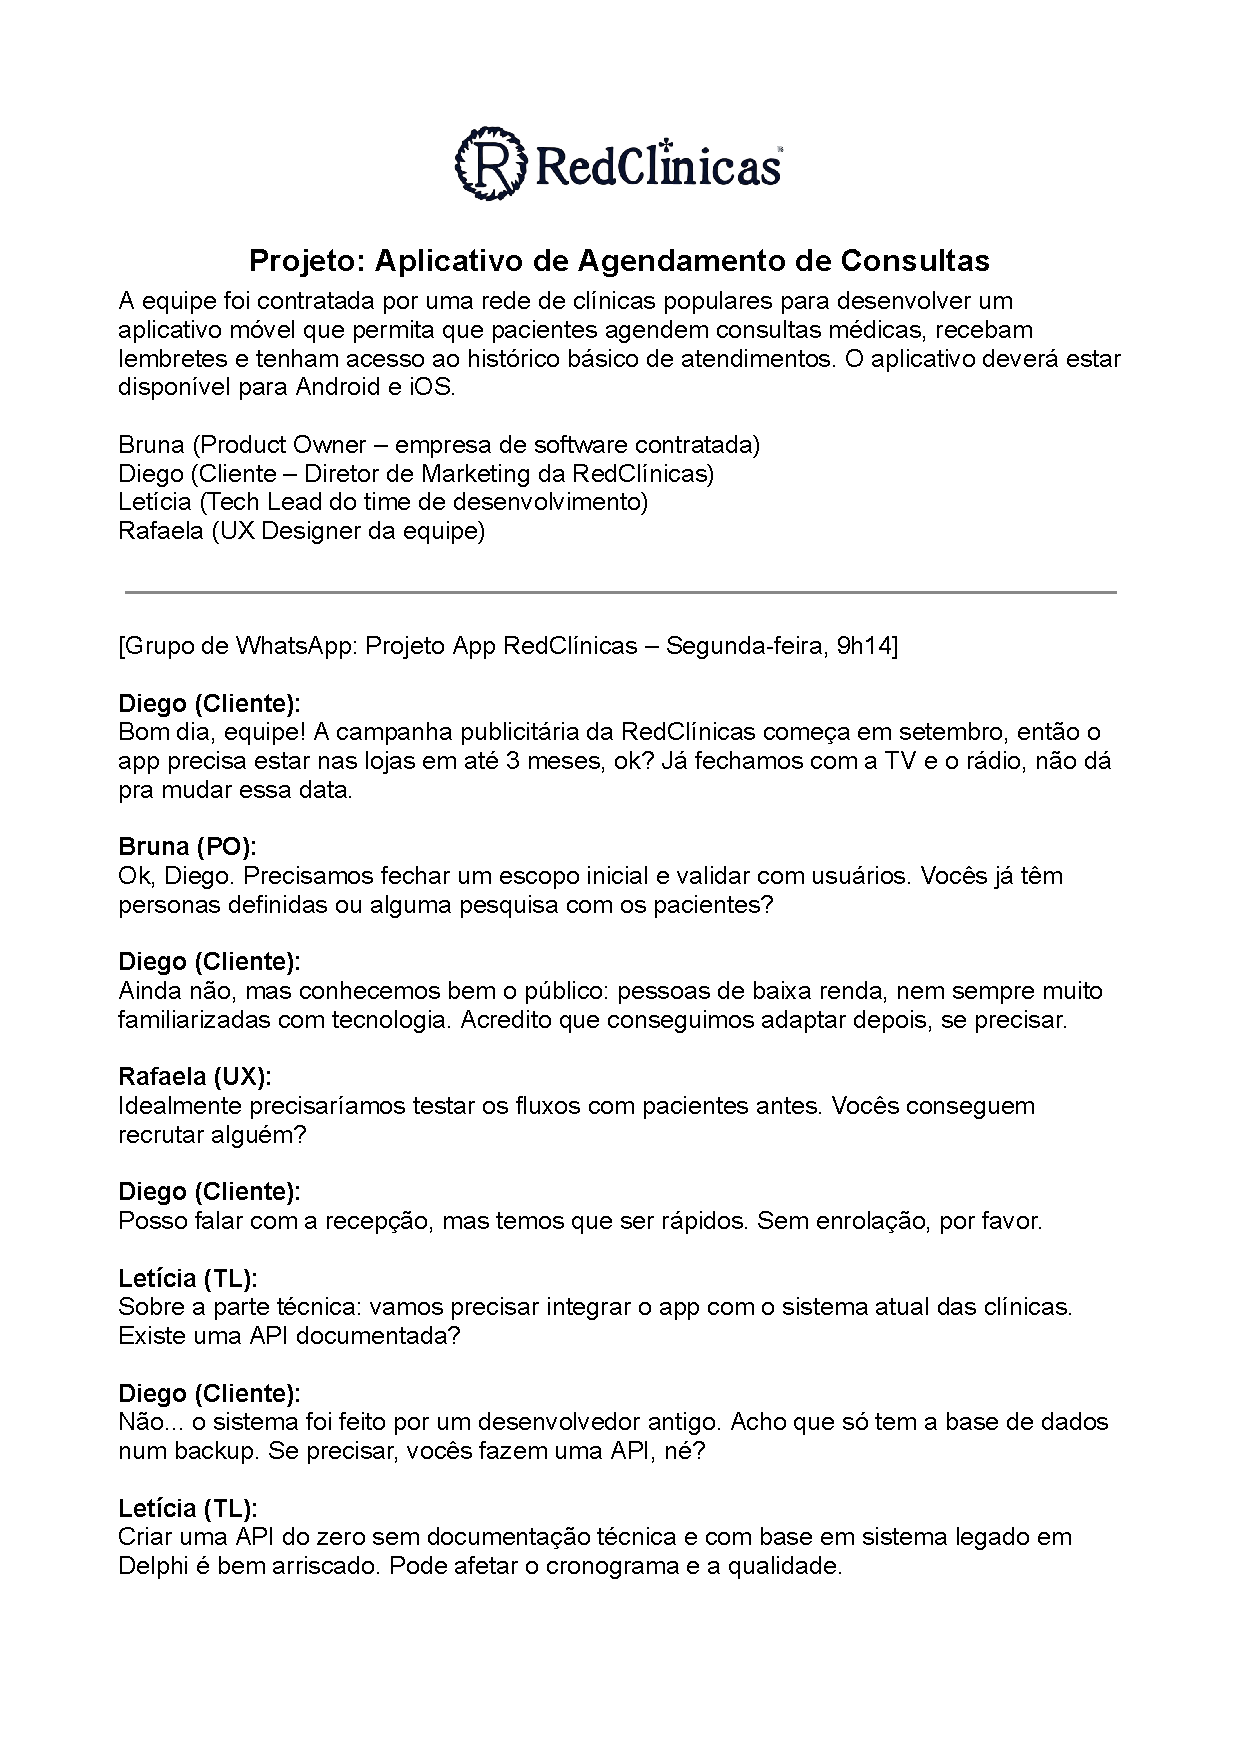
\includepdf[pages=-]{documents/RedClinicas.pdf}
% \centering
% 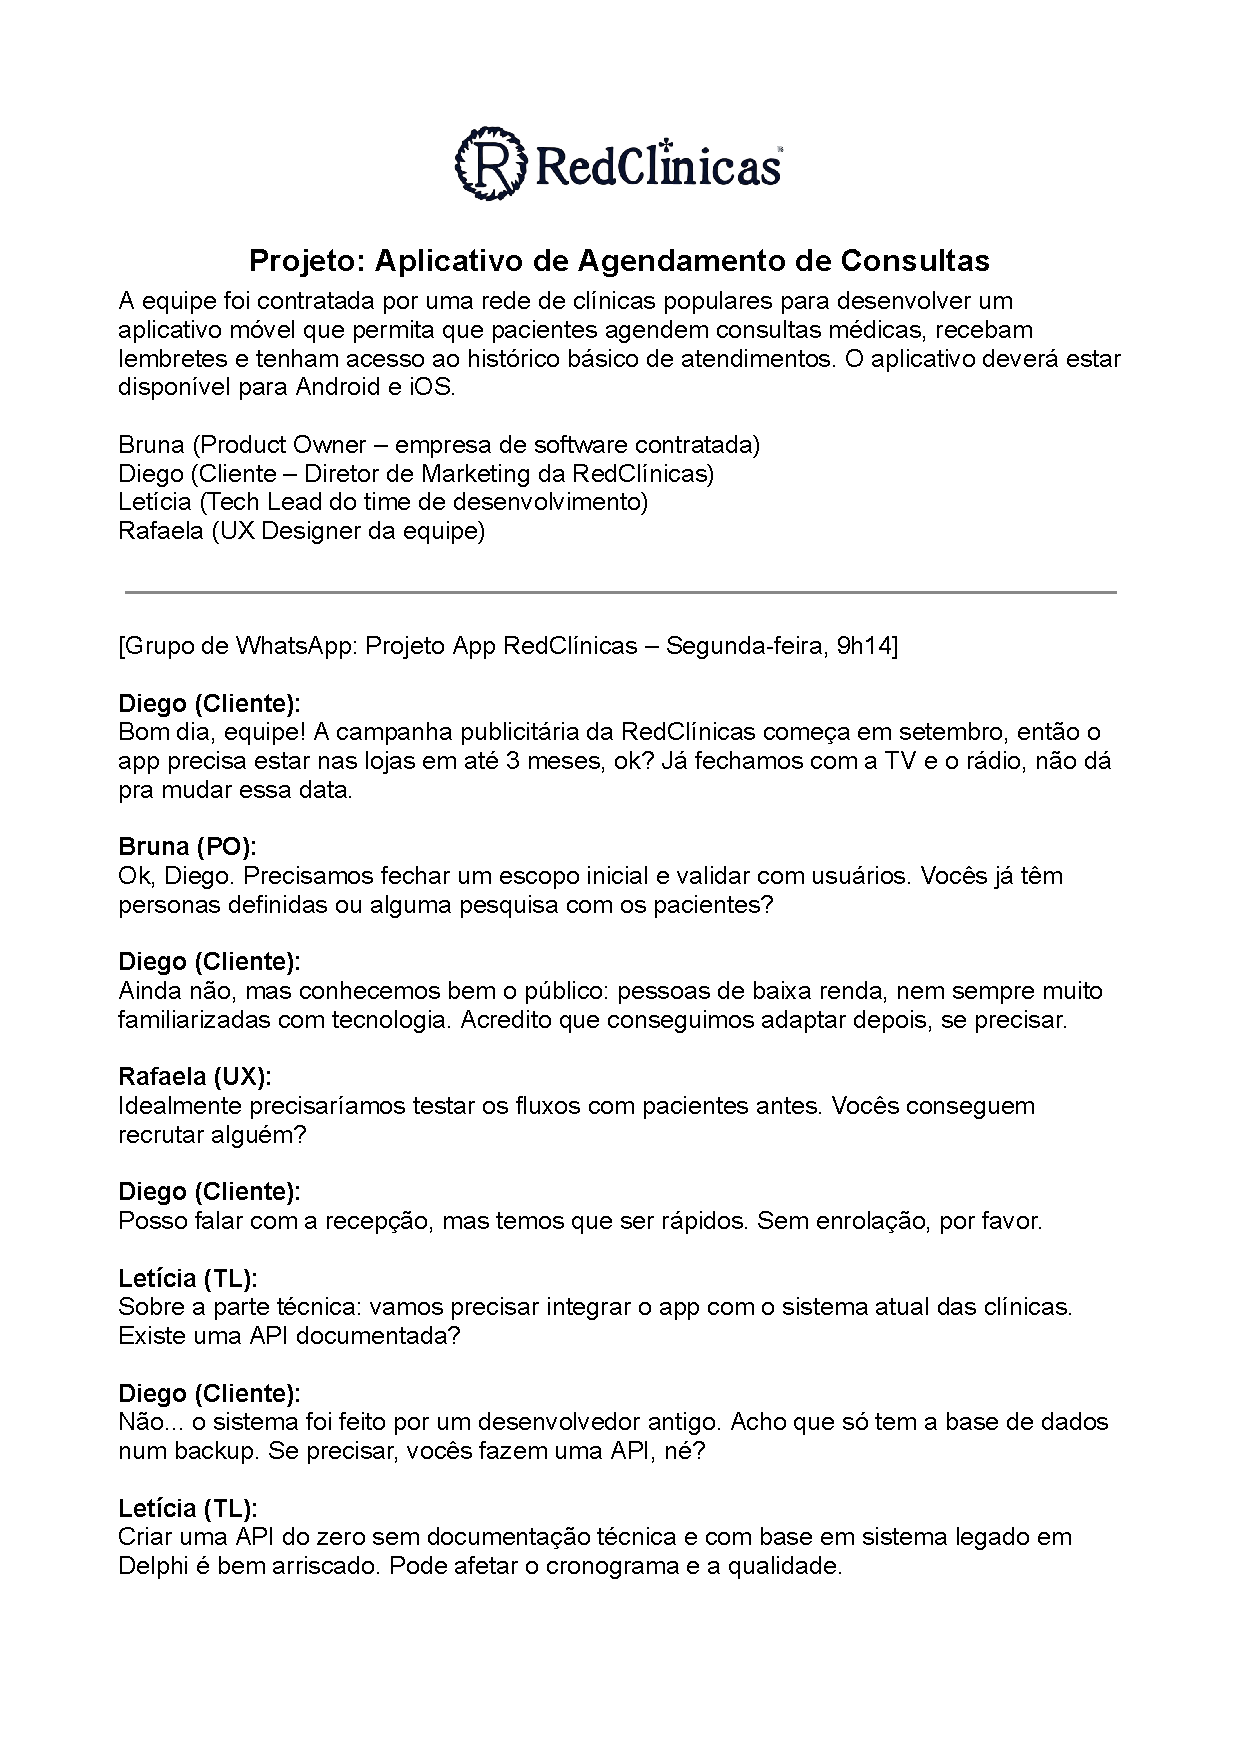
\includegraphics[scale=0.75,page=1]{documents/RedClinicas.pdf}
% \includegraphics[scale=0.75,page=2]{documents/RedClinicas.pdf}

\end{apendices} % Encerra o ambiente de anexos


\phantomsection
\addcontentsline{toc}{chapter}{ANEXOS}
\thispagestyle{empty}
\vspace*{\fill}
\begin{center}
    \textbf{\Huge ANEXOS}
\end{center}
\vspace*{\fill}
\cleardoublepage


\begin{anexos}

\chapter{Declaração de concordância}
\label{anexo:declaracao-concordancia}

\begin{figure}[H]
  \centering
  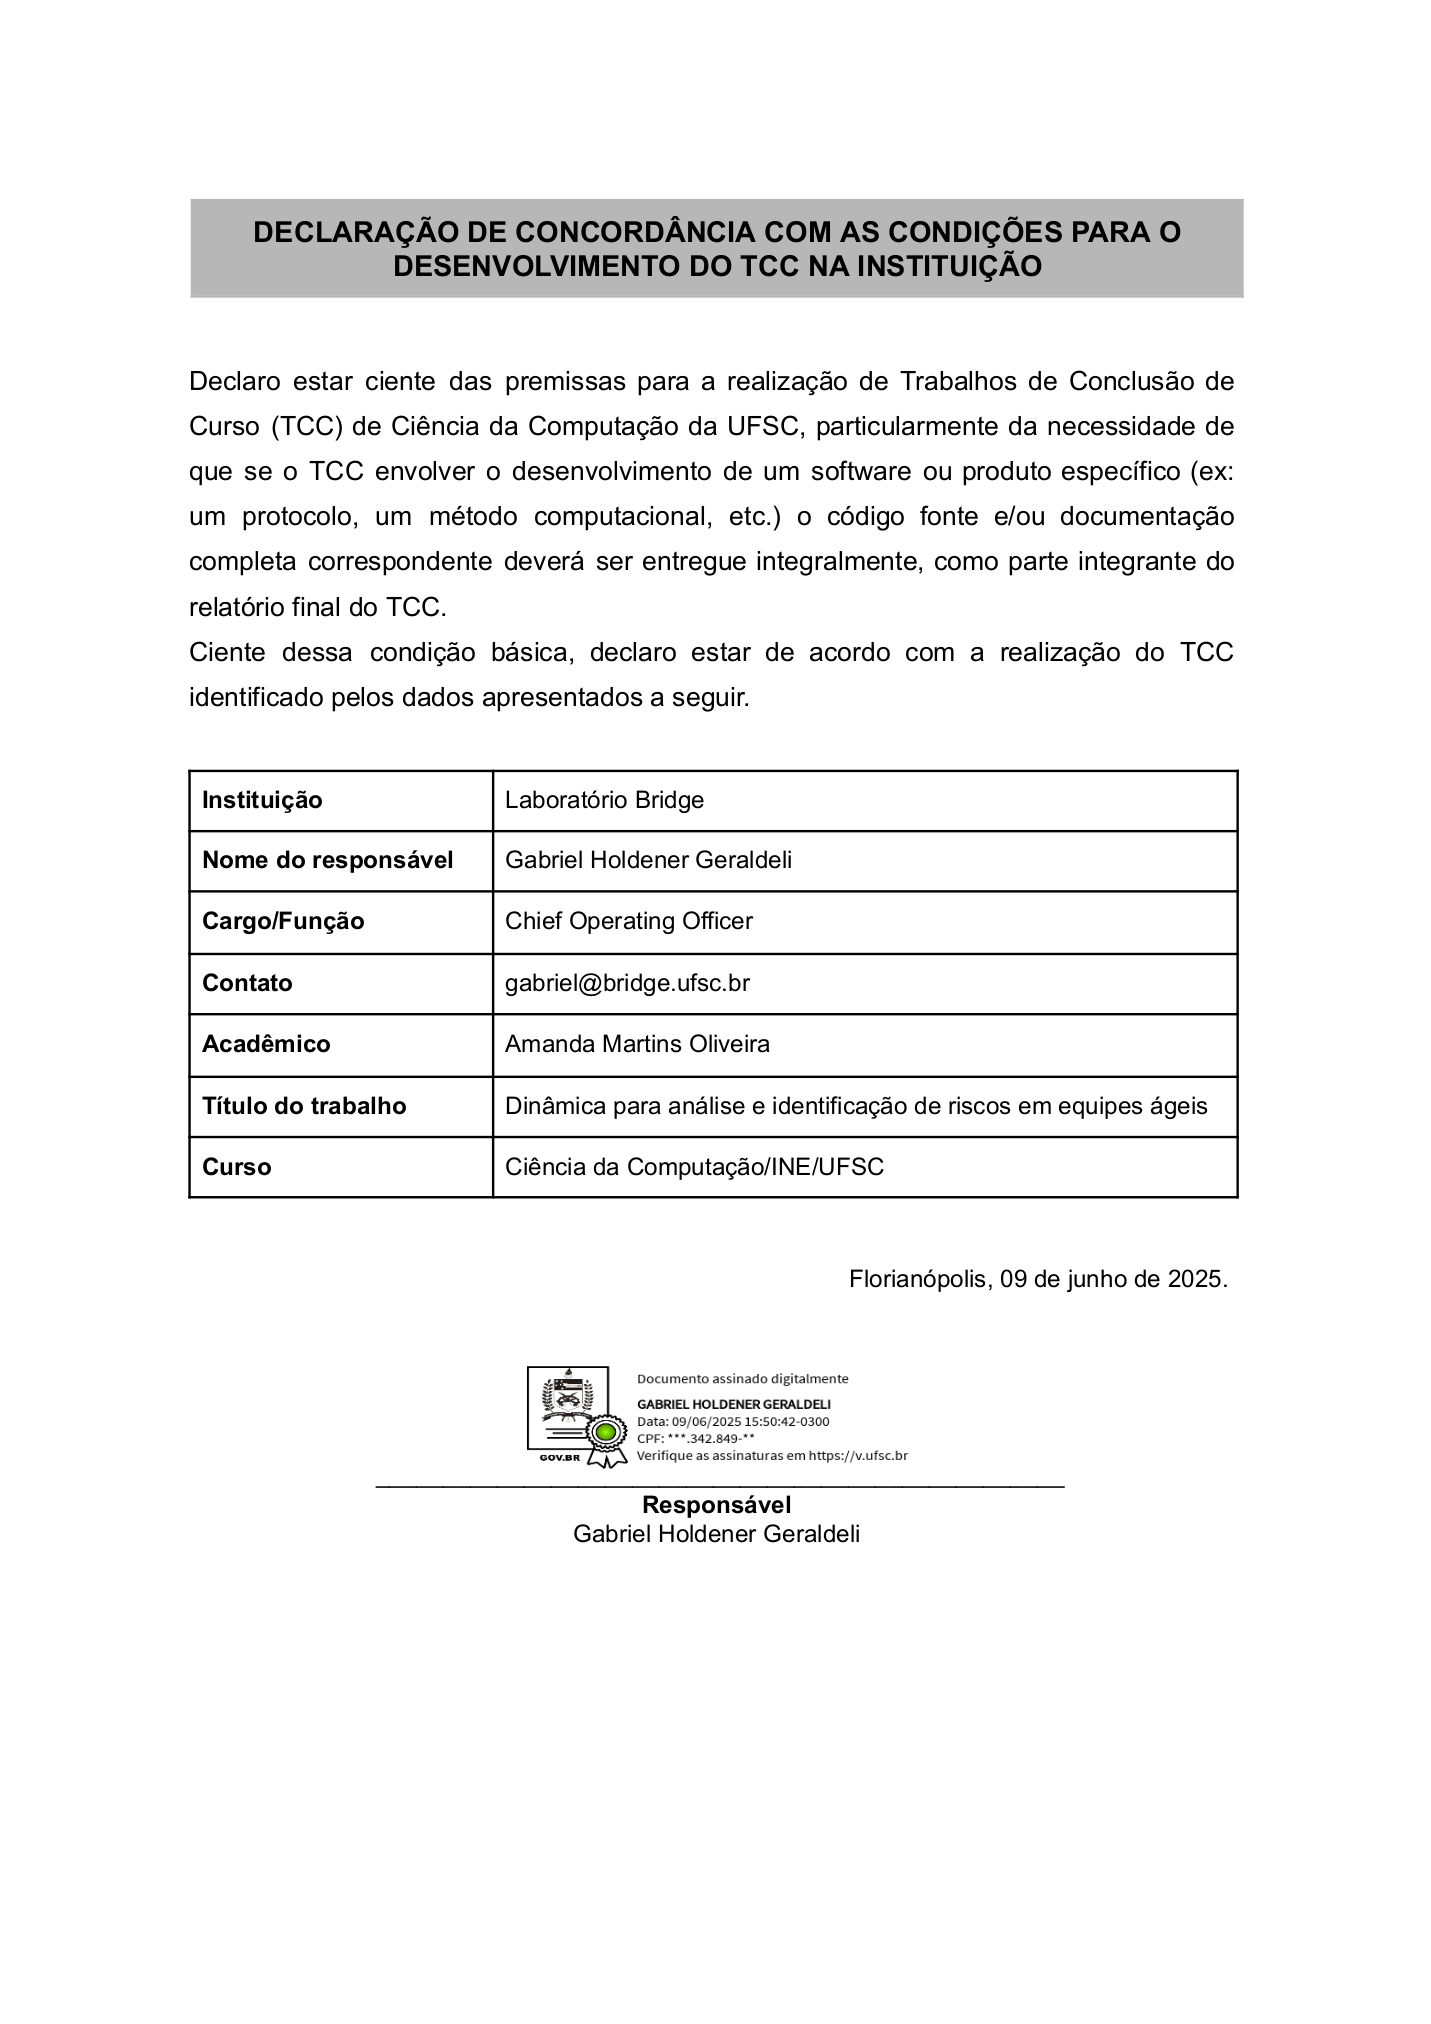
\includegraphics[width=1\textwidth]{print_assinatura}
\end{figure}

%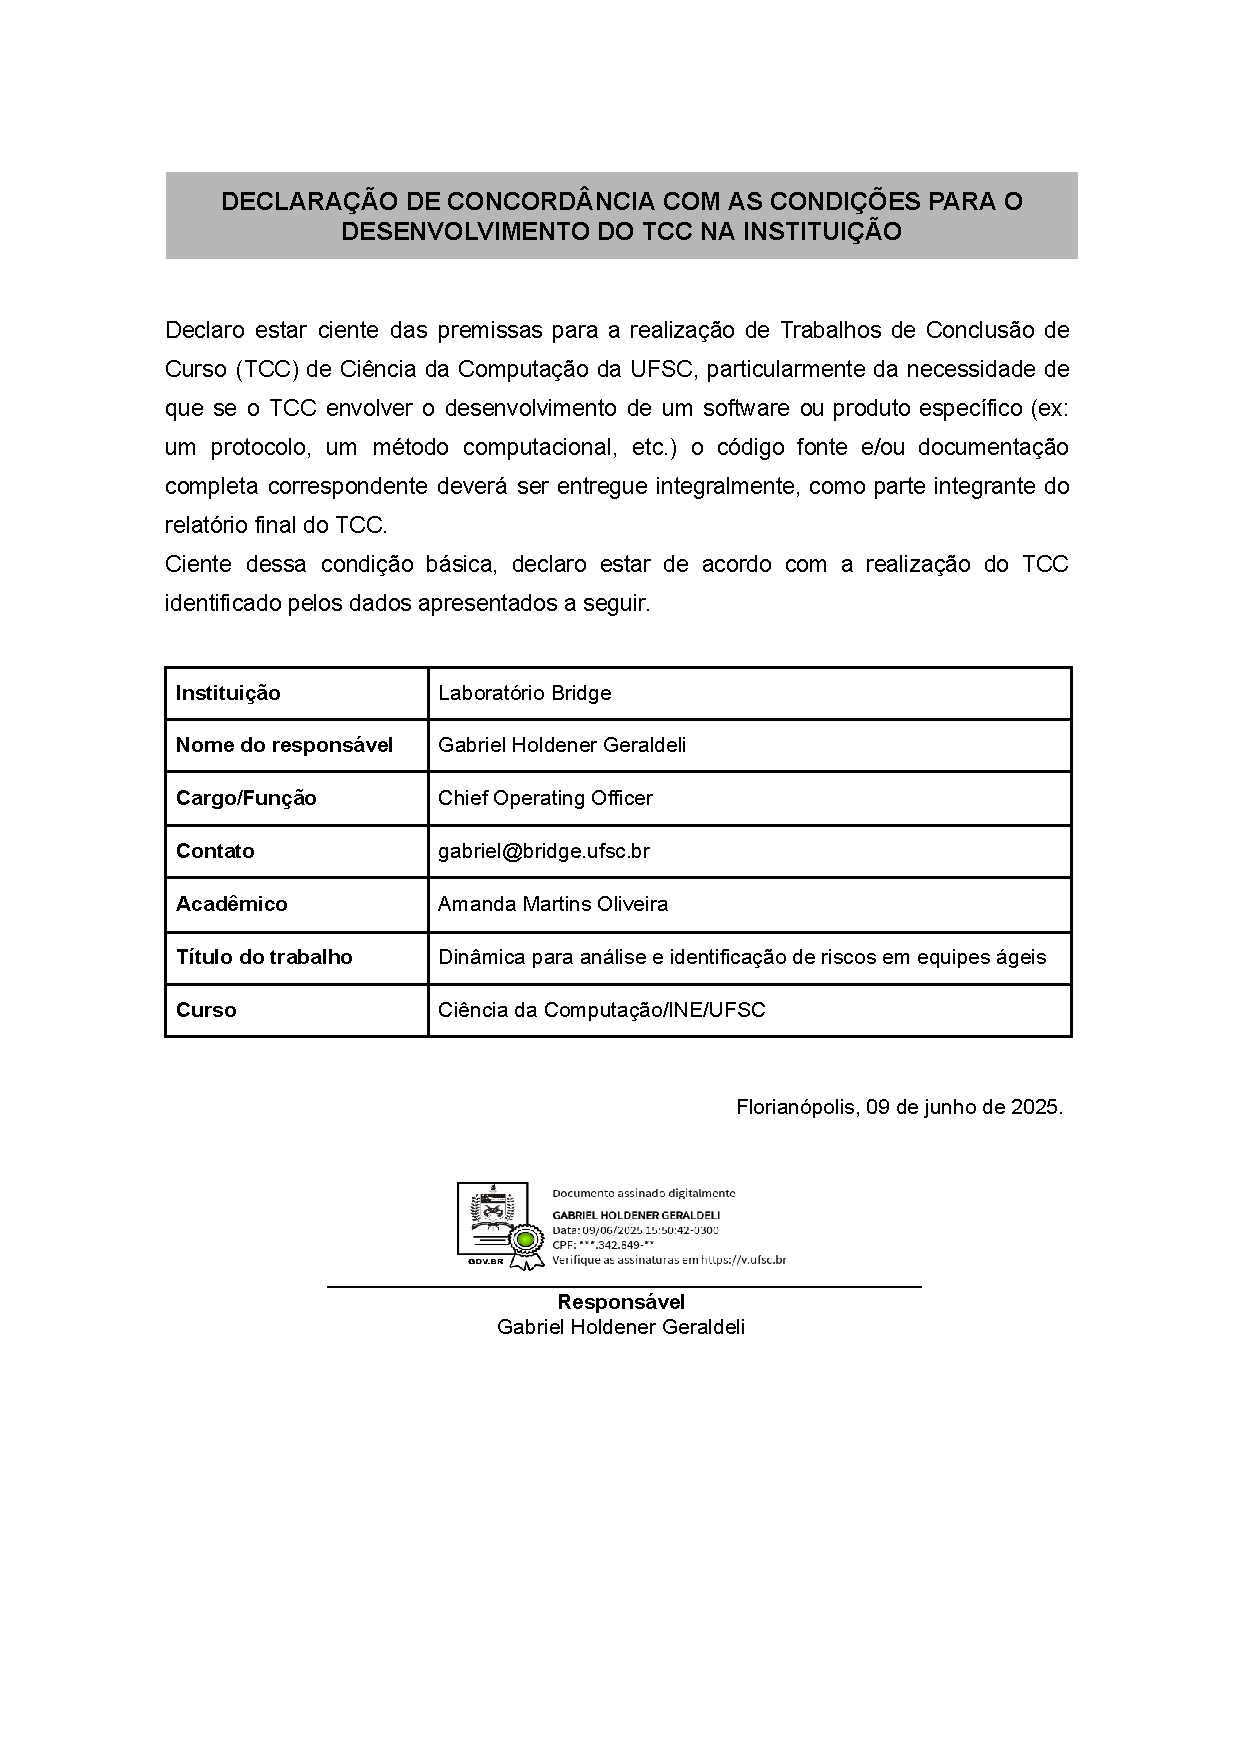
\includepdf[pages={1}]{documents/declaracao_concordancia.pdf}

\end{anexos}

%------------------------------------------------------------------------------%

\phantompart
\printindex

%------------------------------------------------------------------------------%

\end{document}